% Generated by Sphinx.
\def\sphinxdocclass{report}
\documentclass[a4paper,10pt,english]{sphinxmanual}
\usepackage[utf8]{inputenc}
\DeclareUnicodeCharacter{00A0}{\nobreakspace}
\usepackage{cmap}
\usepackage[T1]{fontenc}
\usepackage{babel}
\usepackage{times}
\usepackage[Bjarne]{fncychap}
\usepackage{longtable}
\usepackage{sphinx}
\usepackage{multirow}


\addto\captionsenglish{\renewcommand{\figurename}{Fig. }}
\addto\captionsenglish{\renewcommand{\tablename}{Table }}
\floatname{literal-block}{Listing }



\title{itucsdb Documentation}
\date{December 25, 2015}
\release{1.0}
\author{Team Name}
\newcommand{\sphinxlogo}{}
\renewcommand{\releasename}{Release}
\makeindex

\makeatletter
\def\PYG@reset{\let\PYG@it=\relax \let\PYG@bf=\relax%
    \let\PYG@ul=\relax \let\PYG@tc=\relax%
    \let\PYG@bc=\relax \let\PYG@ff=\relax}
\def\PYG@tok#1{\csname PYG@tok@#1\endcsname}
\def\PYG@toks#1+{\ifx\relax#1\empty\else%
    \PYG@tok{#1}\expandafter\PYG@toks\fi}
\def\PYG@do#1{\PYG@bc{\PYG@tc{\PYG@ul{%
    \PYG@it{\PYG@bf{\PYG@ff{#1}}}}}}}
\def\PYG#1#2{\PYG@reset\PYG@toks#1+\relax+\PYG@do{#2}}

\expandafter\def\csname PYG@tok@gd\endcsname{\def\PYG@tc##1{\textcolor[rgb]{0.63,0.00,0.00}{##1}}}
\expandafter\def\csname PYG@tok@gu\endcsname{\let\PYG@bf=\textbf\def\PYG@tc##1{\textcolor[rgb]{0.50,0.00,0.50}{##1}}}
\expandafter\def\csname PYG@tok@gt\endcsname{\def\PYG@tc##1{\textcolor[rgb]{0.00,0.27,0.87}{##1}}}
\expandafter\def\csname PYG@tok@gs\endcsname{\let\PYG@bf=\textbf}
\expandafter\def\csname PYG@tok@gr\endcsname{\def\PYG@tc##1{\textcolor[rgb]{1.00,0.00,0.00}{##1}}}
\expandafter\def\csname PYG@tok@cm\endcsname{\let\PYG@it=\textit\def\PYG@tc##1{\textcolor[rgb]{0.25,0.50,0.56}{##1}}}
\expandafter\def\csname PYG@tok@vg\endcsname{\def\PYG@tc##1{\textcolor[rgb]{0.73,0.38,0.84}{##1}}}
\expandafter\def\csname PYG@tok@m\endcsname{\def\PYG@tc##1{\textcolor[rgb]{0.13,0.50,0.31}{##1}}}
\expandafter\def\csname PYG@tok@mh\endcsname{\def\PYG@tc##1{\textcolor[rgb]{0.13,0.50,0.31}{##1}}}
\expandafter\def\csname PYG@tok@cs\endcsname{\def\PYG@tc##1{\textcolor[rgb]{0.25,0.50,0.56}{##1}}\def\PYG@bc##1{\setlength{\fboxsep}{0pt}\colorbox[rgb]{1.00,0.94,0.94}{\strut ##1}}}
\expandafter\def\csname PYG@tok@ge\endcsname{\let\PYG@it=\textit}
\expandafter\def\csname PYG@tok@vc\endcsname{\def\PYG@tc##1{\textcolor[rgb]{0.73,0.38,0.84}{##1}}}
\expandafter\def\csname PYG@tok@il\endcsname{\def\PYG@tc##1{\textcolor[rgb]{0.13,0.50,0.31}{##1}}}
\expandafter\def\csname PYG@tok@go\endcsname{\def\PYG@tc##1{\textcolor[rgb]{0.20,0.20,0.20}{##1}}}
\expandafter\def\csname PYG@tok@cp\endcsname{\def\PYG@tc##1{\textcolor[rgb]{0.00,0.44,0.13}{##1}}}
\expandafter\def\csname PYG@tok@gi\endcsname{\def\PYG@tc##1{\textcolor[rgb]{0.00,0.63,0.00}{##1}}}
\expandafter\def\csname PYG@tok@gh\endcsname{\let\PYG@bf=\textbf\def\PYG@tc##1{\textcolor[rgb]{0.00,0.00,0.50}{##1}}}
\expandafter\def\csname PYG@tok@ni\endcsname{\let\PYG@bf=\textbf\def\PYG@tc##1{\textcolor[rgb]{0.84,0.33,0.22}{##1}}}
\expandafter\def\csname PYG@tok@nl\endcsname{\let\PYG@bf=\textbf\def\PYG@tc##1{\textcolor[rgb]{0.00,0.13,0.44}{##1}}}
\expandafter\def\csname PYG@tok@nn\endcsname{\let\PYG@bf=\textbf\def\PYG@tc##1{\textcolor[rgb]{0.05,0.52,0.71}{##1}}}
\expandafter\def\csname PYG@tok@no\endcsname{\def\PYG@tc##1{\textcolor[rgb]{0.38,0.68,0.84}{##1}}}
\expandafter\def\csname PYG@tok@na\endcsname{\def\PYG@tc##1{\textcolor[rgb]{0.25,0.44,0.63}{##1}}}
\expandafter\def\csname PYG@tok@nb\endcsname{\def\PYG@tc##1{\textcolor[rgb]{0.00,0.44,0.13}{##1}}}
\expandafter\def\csname PYG@tok@nc\endcsname{\let\PYG@bf=\textbf\def\PYG@tc##1{\textcolor[rgb]{0.05,0.52,0.71}{##1}}}
\expandafter\def\csname PYG@tok@nd\endcsname{\let\PYG@bf=\textbf\def\PYG@tc##1{\textcolor[rgb]{0.33,0.33,0.33}{##1}}}
\expandafter\def\csname PYG@tok@ne\endcsname{\def\PYG@tc##1{\textcolor[rgb]{0.00,0.44,0.13}{##1}}}
\expandafter\def\csname PYG@tok@nf\endcsname{\def\PYG@tc##1{\textcolor[rgb]{0.02,0.16,0.49}{##1}}}
\expandafter\def\csname PYG@tok@si\endcsname{\let\PYG@it=\textit\def\PYG@tc##1{\textcolor[rgb]{0.44,0.63,0.82}{##1}}}
\expandafter\def\csname PYG@tok@s2\endcsname{\def\PYG@tc##1{\textcolor[rgb]{0.25,0.44,0.63}{##1}}}
\expandafter\def\csname PYG@tok@vi\endcsname{\def\PYG@tc##1{\textcolor[rgb]{0.73,0.38,0.84}{##1}}}
\expandafter\def\csname PYG@tok@nt\endcsname{\let\PYG@bf=\textbf\def\PYG@tc##1{\textcolor[rgb]{0.02,0.16,0.45}{##1}}}
\expandafter\def\csname PYG@tok@nv\endcsname{\def\PYG@tc##1{\textcolor[rgb]{0.73,0.38,0.84}{##1}}}
\expandafter\def\csname PYG@tok@s1\endcsname{\def\PYG@tc##1{\textcolor[rgb]{0.25,0.44,0.63}{##1}}}
\expandafter\def\csname PYG@tok@gp\endcsname{\let\PYG@bf=\textbf\def\PYG@tc##1{\textcolor[rgb]{0.78,0.36,0.04}{##1}}}
\expandafter\def\csname PYG@tok@sh\endcsname{\def\PYG@tc##1{\textcolor[rgb]{0.25,0.44,0.63}{##1}}}
\expandafter\def\csname PYG@tok@ow\endcsname{\let\PYG@bf=\textbf\def\PYG@tc##1{\textcolor[rgb]{0.00,0.44,0.13}{##1}}}
\expandafter\def\csname PYG@tok@sx\endcsname{\def\PYG@tc##1{\textcolor[rgb]{0.78,0.36,0.04}{##1}}}
\expandafter\def\csname PYG@tok@bp\endcsname{\def\PYG@tc##1{\textcolor[rgb]{0.00,0.44,0.13}{##1}}}
\expandafter\def\csname PYG@tok@c1\endcsname{\let\PYG@it=\textit\def\PYG@tc##1{\textcolor[rgb]{0.25,0.50,0.56}{##1}}}
\expandafter\def\csname PYG@tok@kc\endcsname{\let\PYG@bf=\textbf\def\PYG@tc##1{\textcolor[rgb]{0.00,0.44,0.13}{##1}}}
\expandafter\def\csname PYG@tok@c\endcsname{\let\PYG@it=\textit\def\PYG@tc##1{\textcolor[rgb]{0.25,0.50,0.56}{##1}}}
\expandafter\def\csname PYG@tok@mf\endcsname{\def\PYG@tc##1{\textcolor[rgb]{0.13,0.50,0.31}{##1}}}
\expandafter\def\csname PYG@tok@err\endcsname{\def\PYG@bc##1{\setlength{\fboxsep}{0pt}\fcolorbox[rgb]{1.00,0.00,0.00}{1,1,1}{\strut ##1}}}
\expandafter\def\csname PYG@tok@mb\endcsname{\def\PYG@tc##1{\textcolor[rgb]{0.13,0.50,0.31}{##1}}}
\expandafter\def\csname PYG@tok@ss\endcsname{\def\PYG@tc##1{\textcolor[rgb]{0.32,0.47,0.09}{##1}}}
\expandafter\def\csname PYG@tok@sr\endcsname{\def\PYG@tc##1{\textcolor[rgb]{0.14,0.33,0.53}{##1}}}
\expandafter\def\csname PYG@tok@mo\endcsname{\def\PYG@tc##1{\textcolor[rgb]{0.13,0.50,0.31}{##1}}}
\expandafter\def\csname PYG@tok@kd\endcsname{\let\PYG@bf=\textbf\def\PYG@tc##1{\textcolor[rgb]{0.00,0.44,0.13}{##1}}}
\expandafter\def\csname PYG@tok@mi\endcsname{\def\PYG@tc##1{\textcolor[rgb]{0.13,0.50,0.31}{##1}}}
\expandafter\def\csname PYG@tok@kn\endcsname{\let\PYG@bf=\textbf\def\PYG@tc##1{\textcolor[rgb]{0.00,0.44,0.13}{##1}}}
\expandafter\def\csname PYG@tok@o\endcsname{\def\PYG@tc##1{\textcolor[rgb]{0.40,0.40,0.40}{##1}}}
\expandafter\def\csname PYG@tok@kr\endcsname{\let\PYG@bf=\textbf\def\PYG@tc##1{\textcolor[rgb]{0.00,0.44,0.13}{##1}}}
\expandafter\def\csname PYG@tok@s\endcsname{\def\PYG@tc##1{\textcolor[rgb]{0.25,0.44,0.63}{##1}}}
\expandafter\def\csname PYG@tok@kp\endcsname{\def\PYG@tc##1{\textcolor[rgb]{0.00,0.44,0.13}{##1}}}
\expandafter\def\csname PYG@tok@w\endcsname{\def\PYG@tc##1{\textcolor[rgb]{0.73,0.73,0.73}{##1}}}
\expandafter\def\csname PYG@tok@kt\endcsname{\def\PYG@tc##1{\textcolor[rgb]{0.56,0.13,0.00}{##1}}}
\expandafter\def\csname PYG@tok@sc\endcsname{\def\PYG@tc##1{\textcolor[rgb]{0.25,0.44,0.63}{##1}}}
\expandafter\def\csname PYG@tok@sb\endcsname{\def\PYG@tc##1{\textcolor[rgb]{0.25,0.44,0.63}{##1}}}
\expandafter\def\csname PYG@tok@k\endcsname{\let\PYG@bf=\textbf\def\PYG@tc##1{\textcolor[rgb]{0.00,0.44,0.13}{##1}}}
\expandafter\def\csname PYG@tok@se\endcsname{\let\PYG@bf=\textbf\def\PYG@tc##1{\textcolor[rgb]{0.25,0.44,0.63}{##1}}}
\expandafter\def\csname PYG@tok@sd\endcsname{\let\PYG@it=\textit\def\PYG@tc##1{\textcolor[rgb]{0.25,0.44,0.63}{##1}}}

\def\PYGZbs{\char`\\}
\def\PYGZus{\char`\_}
\def\PYGZob{\char`\{}
\def\PYGZcb{\char`\}}
\def\PYGZca{\char`\^}
\def\PYGZam{\char`\&}
\def\PYGZlt{\char`\<}
\def\PYGZgt{\char`\>}
\def\PYGZsh{\char`\#}
\def\PYGZpc{\char`\%}
\def\PYGZdl{\char`\$}
\def\PYGZhy{\char`\-}
\def\PYGZsq{\char`\'}
\def\PYGZdq{\char`\"}
\def\PYGZti{\char`\~}
% for compatibility with earlier versions
\def\PYGZat{@}
\def\PYGZlb{[}
\def\PYGZrb{]}
\makeatother

\renewcommand\PYGZsq{\textquotesingle}

\begin{document}

\maketitle
\tableofcontents
\phantomsection\label{index::doc}

\begin{quote}\begin{description}
\item[{Team}] \leavevmode
itucsdb1525

\item[{Members}] \leavevmode\begin{itemize}
\item {} 
Member 1

\item {} 
Cemal Türkoğlu

\item {} 
Member 3

\item {} 
Ercan Alp Serteli

\item {} 
Member 5

\end{itemize}

\end{description}\end{quote}

\textbf{project description goes here (a few paragraphs)}

Contents:


\chapter{User Guide}
\label{user/index:user-guide}\label{user/index:welcome-to-itucsdb1525-s-documentation}\label{user/index::doc}
\textbf{explain how your application works from the user perspective, use
screenshots whereever appropriate}

\textbf{to add a picture, use the following example}:

\begin{Verbatim}[commandchars=\\\{\}]
.. figure:: picture.png
   :scale: 50 \PYGZpc{}
   :alt: map to buried treasure

   This is the caption of the figure (a simple paragraph).
\end{Verbatim}


\section{Parts Implemented by Member Name}
\label{user/member1:parts-implemented-by-member-name}\label{user/member1::doc}

\section{Parts Implemented by Cemal Türkoğlu}
\label{user/member2::doc}\label{user/member2:parts-implemented-by-cemal-turkoglu}
The parts that I have implemented are the \emph{Power Boat Racing} pages and functionalities related to users.


\subsection{Power Boat Racing}
\label{user/member2:power-boat-racing}
The power boat racing pages can be reached by clicking this button in the home page.
\begin{quote}

\scalebox{0.800000}{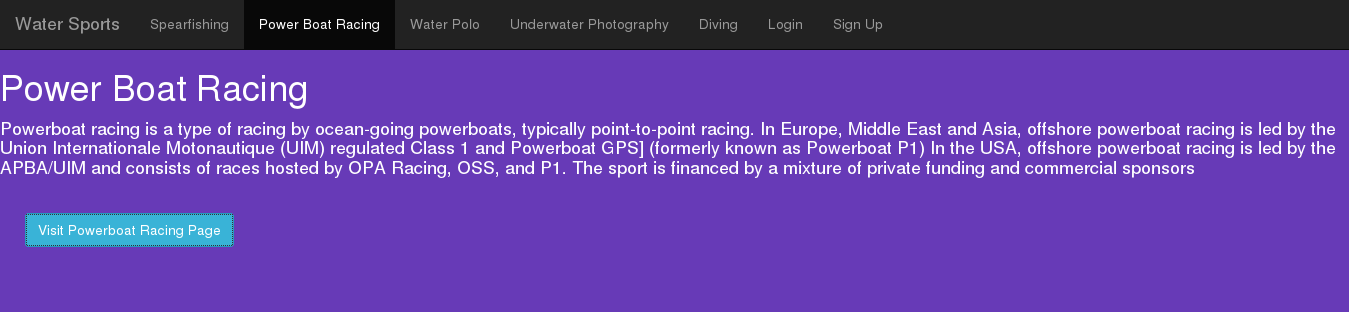
\includegraphics{visit.png}}
\end{quote}

Power boat racing pages locates under /drivers route. In the main page you can see some complex statistics
and all tables. There are 5 table: Drivers,Teams,Boats,League15,OldRaces. In table operation you can make
add,delete,update and resetting table


\subsubsection{Adding}
\label{user/member2:adding}
To add a new driver, you need to enter a name,team and boat using the textboxes.Also click the \emph{Add} button.
\begin{quote}

\scalebox{1.000000}{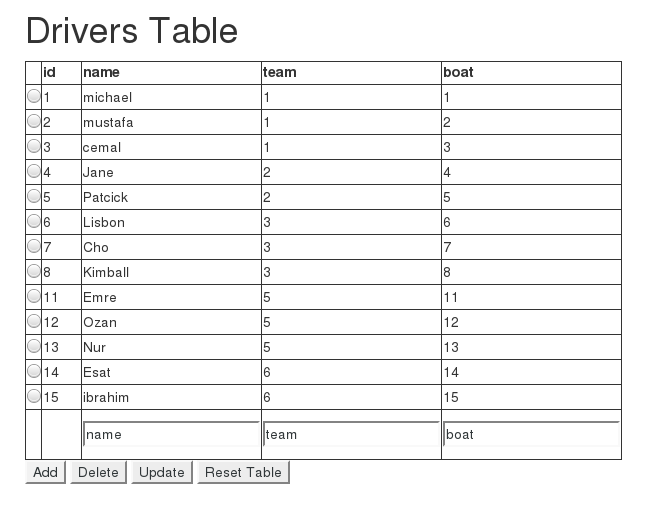
\includegraphics{add.png}}
\end{quote}

As a result, the new driver you entered will be added to the database and the new list will be shown to you.


\subsubsection{Deleting}
\label{user/member2:deleting}
To delete a driver, click the circle to its left in the list. Then press the \emph{Delete} button.
\begin{quote}

\scalebox{1.000000}{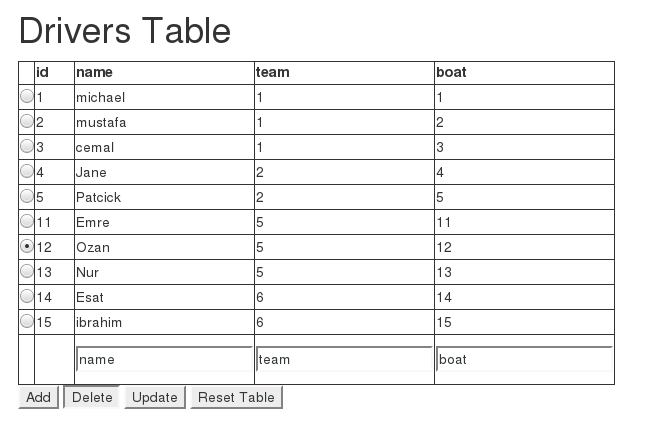
\includegraphics{delete.png}}

\begin{notice}{note}{Note:}
If you try to break referencial integrity , it will not be allowed.
\end{notice}
\end{quote}

Then, the entry will be removed from the database and the resulting list will be displayed.


\subsubsection{Updating}
\label{user/member2:updating}
To update the information of a competitor, select the comptitor in the same manner as deleting (by clicking the circle to its left) and then enter the information as you would in adding. After that, click the \emph{Update} button and watch it happen.
\begin{quote}

\scalebox{1.000000}{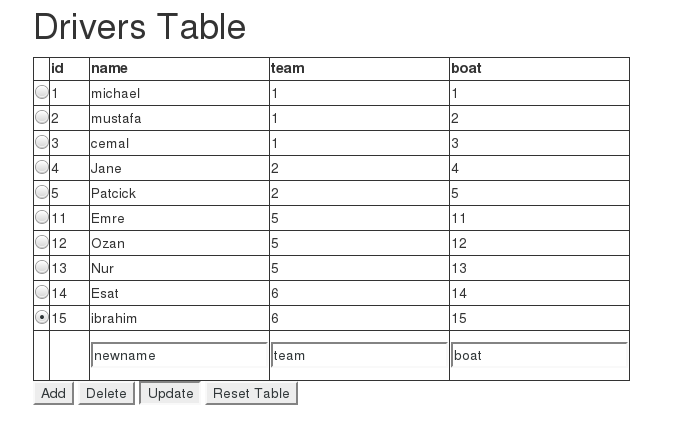
\includegraphics{update.png}}
\end{quote}

Information in the entry will be updated and shown back.
\begin{quote}

\begin{notice}{note}{Note:}
Again breaking referencial integrity is not allowed
\end{notice}
\end{quote}


\subsubsection{Resetting the Table}
\label{user/member2:resetting-the-table}
Clicking the \emph{Reset Table} button reverts any changes done to both the competitors and the teams table and fills them with default values. Not much has to be said about this function.


\subsubsection{Tables}
\label{user/member2:tables}\begin{description}
\item[{All tables are listed in main page.Also from the left menu one of the table can be selected to display.}] \leavevmode
Drivers

\scalebox{1.000000}{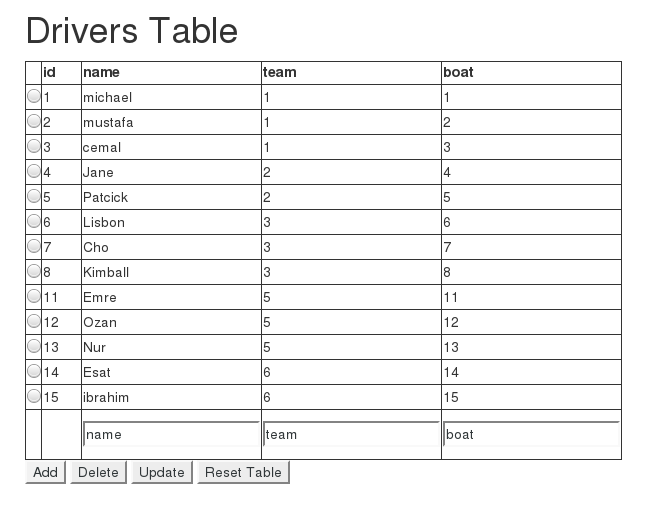
\includegraphics{add.png}}

Teams

\scalebox{1.000000}{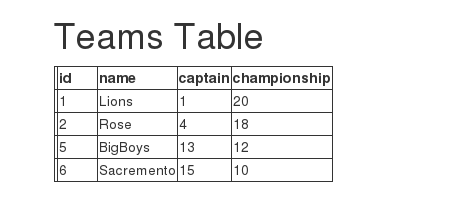
\includegraphics{teams.png}}

Boats

\scalebox{1.000000}{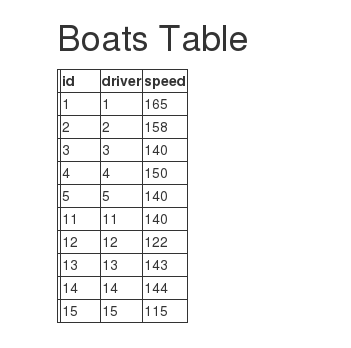
\includegraphics{boats.png}}

League

\scalebox{1.000000}{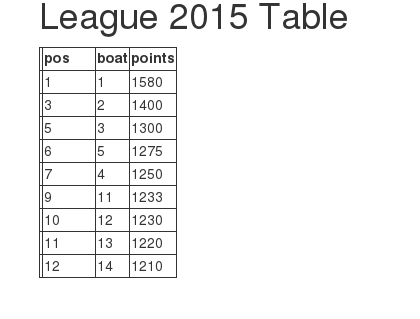
\includegraphics{league.png}}

OldRaces

\scalebox{1.000000}{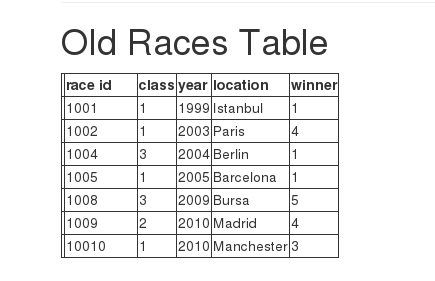
\includegraphics{oldraces.png}}

\end{description}


\section{Parts Implemented by Member Name}
\label{user/member3:parts-implemented-by-member-name}\label{user/member3::doc}

\section{Parts Implemented by Ercan Alp Serteli}
\label{user/member4:parts-implemented-by-ercan-alp-serteli}\label{user/member4::doc}
The parts that I have implemented are the \emph{Underwater Photography} pages and functionalities related to users.


\subsection{Underwater Photography}
\label{user/member4:underwater-photography}
The underwater photography pages can be reached by clicking this button in the home page.
\begin{quote}

\scalebox{0.800000}{
\includegraphics{visit_button.PNG}}
\end{quote}

Or from this menu item in the navigation bar from any other page.
\begin{quote}

\scalebox{1.000000}{
\includegraphics{navbar_button.PNG}}
\end{quote}

Now that you clicked one of them, you are in the \emph{Competitors} page of Underwater Photography.
\begin{quote}

\scalebox{1.000000}{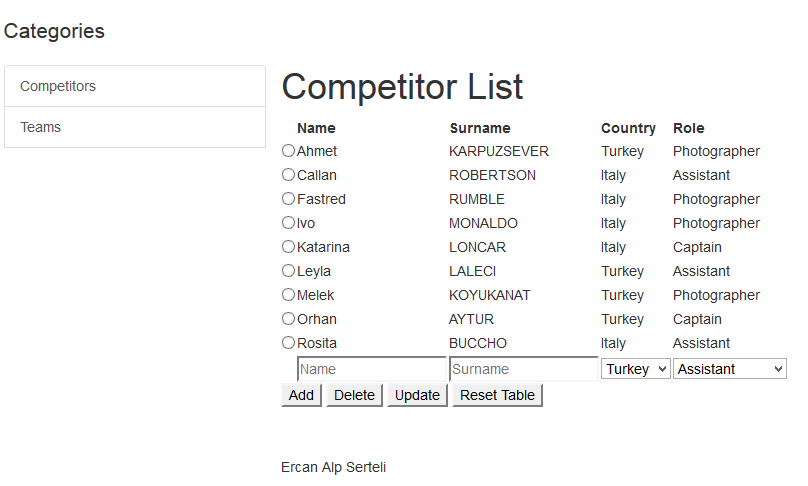
\includegraphics{competitor_page.PNG}}
\end{quote}

From the \emph{Categories} menu you see on the left, it is possible to navigate between the two pages of Underwater Photography: \emph{Competitors} and \emph{Teams}

What you see in the middle is a representation of the underlying Competitors database table. It lists the information of the existing competitors in the table and allows anyone to modify the table via adding, updating or deleting entries or via resetting the table to its default state.

The entries are sorted according to the alphabetical order of their first names.


\subsubsection{Adding}
\label{user/member4:adding}
To add a new competitor, you need to enter a name and a surname using the textboxes. Then you need to select a country and a role using the dropdown menus and click the \emph{Add} button.
\begin{quote}

\scalebox{1.000000}{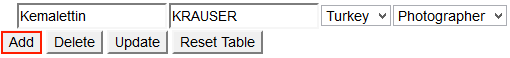
\includegraphics{add.PNG}}

\begin{notice}{note}{Note:}
To add a competitor from a team of some non-existing country, you first need to add the team from the \emph{Teams} page. On the other hand, the team roles are fixed. They cannot be changed and a new role cannot be added.
\end{notice}
\end{quote}

As a result, the new competitor you entered will be added to the database and the new list will be shown to you.
\begin{quote}

\scalebox{1.000000}{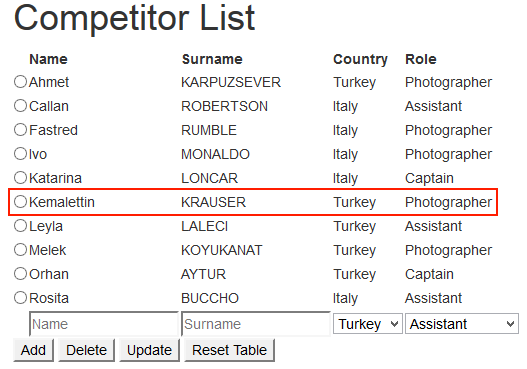
\includegraphics{add_newlist.PNG}}

\begin{notice}{note}{Note:}
If you leave the name or the surname boxes empty, it will not be added and the page will show you a warning message
\end{notice}
\end{quote}


\subsubsection{Deleting}
\label{user/member4:deleting}
To delete a competitor, click the circle to its left in the list. Then press the \emph{Delete} button.
\begin{quote}

\scalebox{1.000000}{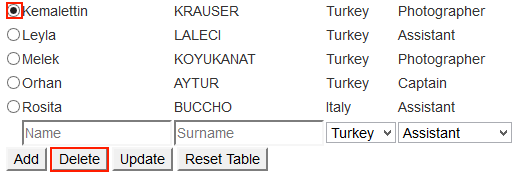
\includegraphics{delete.PNG}}
\end{quote}

Then, the entry will be removed from the database and the resulting list will be displayed.


\subsubsection{Updating}
\label{user/member4:updating}
To update the information of a competitor, select the comptitor in the same manner as deleting (by clicking the circle to its left) and then enter the information as you would in adding. After that, click the \emph{Update} button and watch it happen.
\begin{quote}

\scalebox{1.000000}{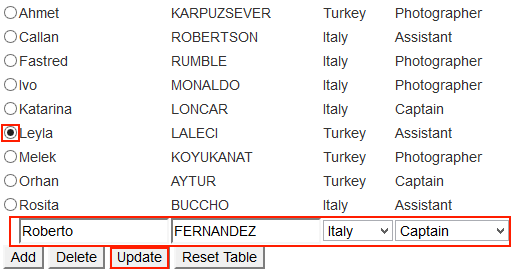
\includegraphics{update.PNG}}
\end{quote}

Information in the entry will be updated and shown back.
\begin{quote}

\scalebox{1.000000}{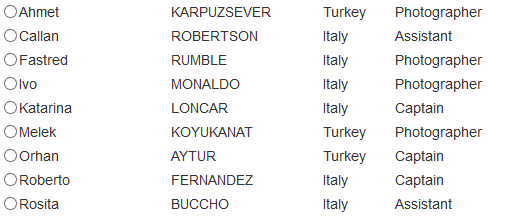
\includegraphics{update_newlist.PNG}}
\end{quote}


\subsubsection{Resetting the Table}
\label{user/member4:resetting-the-table}
Clicking the \emph{Reset Table} button reverts any changes done to both the competitors and the teams table and fills them with default values. Not much has to be said about this function.


\subsubsection{Teams Page}
\label{user/member4:teams-page}
When you click the \emph{Teams} button in the left menu, you will end up in this page.
\begin{quote}

\scalebox{1.000000}{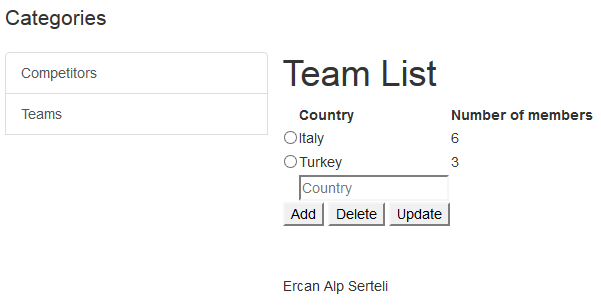
\includegraphics{teams.PNG}}
\end{quote}

What you see is the same structure as the Competitors page, but with a smaller table. That is the teams list. Teams only have a \emph{Country} field and an ID, since competitions are held with national teams. In fact, the competitors list you have seen before is taking its country information from this table.

All the operations as in the Competitors page are possible here as well, and they all work the same.
\begin{quote}

\begin{notice}{note}{Note:}
If you try to delete a team that has members in the competitors list, you cannot do it. To do this, delete the members from the Competitors page first.
\end{notice}
\end{quote}


\subsection{User Operations}
\label{user/member4:user-operations}
The website supports basic user functionalities such as signing up, logging in, logging out. Modifying the information of users is also possible for admin type accounts.


\subsubsection{Signing up}
\label{user/member4:signing-up}
You can move to the sign up page by clicking the \emph{Sign Up} button from the navigation bar.
\begin{quote}

\scalebox{0.800000}{
\includegraphics{sign_up_button.PNG}}
\end{quote}

In the sign up page, enter a username and a password and press the \emph{Sign Up} button. This will enable you to login using those credentials. You will be redirected to the Login page, since you will probably want to login after signing up.
\begin{quote}

\scalebox{1.000000}{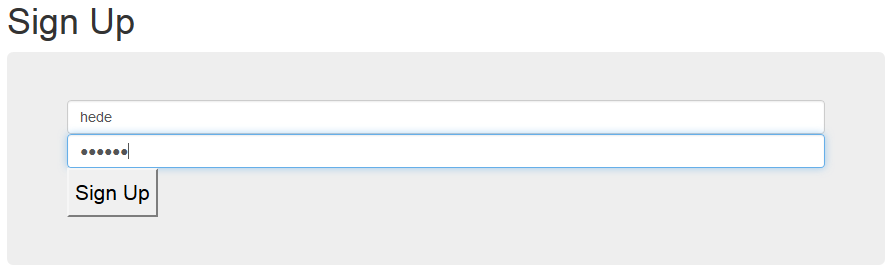
\includegraphics{sign_up_page.PNG}}

\begin{notice}{note}{Note:}
If you try to sign up with a blank username or password, the page will warn you. Also a different warning message will be shown if you enter an username that already exists in the system.
\end{notice}

\begin{notice}{warning}{Warning:}
Do not use a real password to sign up because it is not secure, at all. Literally anyone can see your information if they want to.
\end{notice}
\end{quote}


\subsubsection{Logging in}
\label{user/member4:logging-in}
You can get to the login page by clicking the \emph{Login} button from the navigation bar.
\begin{quote}

\scalebox{0.800000}{
\includegraphics{login_button.PNG}}
\end{quote}

You can also get redirected here by signing up.

You will be given a default admin account's credentials in case you want to try out being an admin. You can login using that or your own credentials.
\begin{quote}

\begin{notice}{note}{Note:}
Any user who signs up is a \emph{User} type user. To change a user's type, you have to be logged in as an \emph{Admin} type user.
\end{notice}

\scalebox{1.000000}{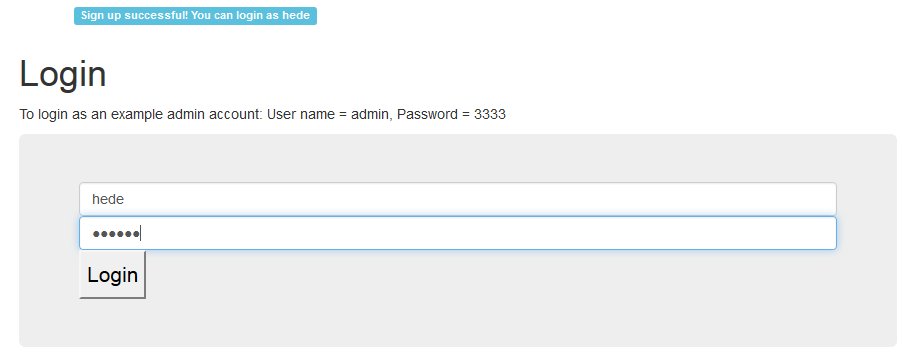
\includegraphics{login_page.PNG}}

\begin{notice}{note}{Note:}
If you try to login using wrong information, the page will show you a message and let you try again.
\end{notice}
\end{quote}


\subsubsection{Logging out}
\label{user/member4:logging-out}
Once you are logged in, a new item appears in the navigation bar while the sign up and login items disappear. This new button lets you log out from the system.
\begin{quote}

\scalebox{0.800000}{
\includegraphics{logout_button.PNG}}
\end{quote}

Once you click it, you will no longer be logged in.


\subsubsection{Users Page}
\label{user/member4:users-page}
If you login as an admin, you will be directed to the \emph{Users} page. You can also go there using the navigation bar item that only shows up if you are an admin.
\begin{quote}

\scalebox{0.800000}{
\includegraphics{users_button.PNG}}
\end{quote}

In the users page, you will see the list of users. You can add, delete or update users or you can reset the users table. The operations are identical to the ones in the Underwater Photography pages.
\begin{quote}

\scalebox{0.800000}{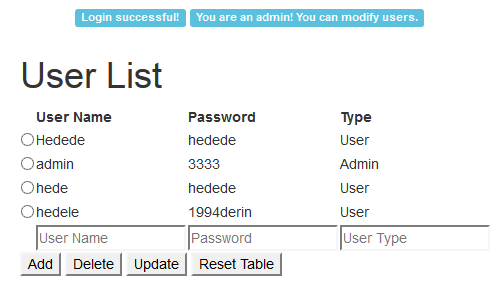
\includegraphics{users_page.PNG}}
\end{quote}


\section{Parts Implemented by Turker Unlu}
\label{user/member5:parts-implemented-by-turker-unlu}\label{user/member5::doc}

\section{Divers}
\label{user/member5:divers}
This section of the page is used for managing information about dive sporters.
\begin{figure}[htbp]
\centering
\capstart

\scalebox{0.300000}{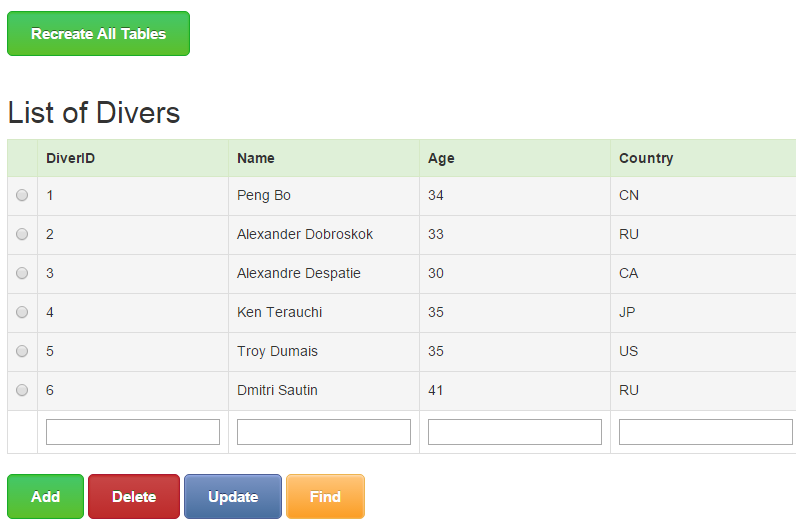
\includegraphics{divertable.png}}
\caption{Fig. 1.1: Screenshot of Divers Table}\end{figure}

Information about divers is listed on the screen.
Data table consist of ID, name, age and country information of the sporter.
ID is unique sporter ID of a sporter.
Name and age are sporter's personal information.
Country is the country sporter represents.

Operations add, delete, update and find can be done from this section alone.


\section{Competitions}
\label{user/member5:competitions}
This section of the page is used for managing information about diving competitions.
\begin{figure}[htbp]
\centering
\capstart

\scalebox{0.300000}{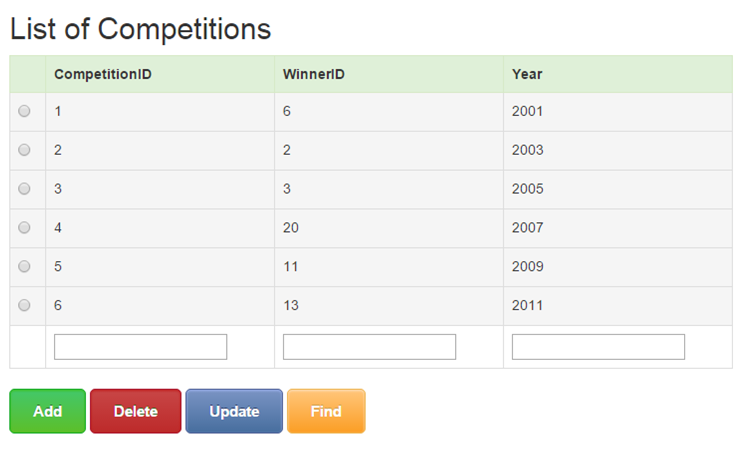
\includegraphics{competitiontable.png}}
\caption{Fig. 1.2: Screenshot of Competition Table}\end{figure}

Information about diving competitions is listed on the screen.
Data table consist of competition ID, winner sporter ID and the year which competition is done.
CompetitionID is the unique ID of a diving competition.
WinnerID is the ID of the sporter who won the competition.
Year is the date which the competition held.

Operations add, delete, update and find can be done from this section alone.
The sporter with the ID number winnerID must exist in order to add a new competition.


\section{Records}
\label{user/member5:records}
This section of the page is used for managing information about a sporter record at a specific competition.
For example sporter ``DiverID'' jumped from 5 meter at competition ``CompetitionID''
\begin{figure}[htbp]
\centering
\capstart

\scalebox{0.300000}{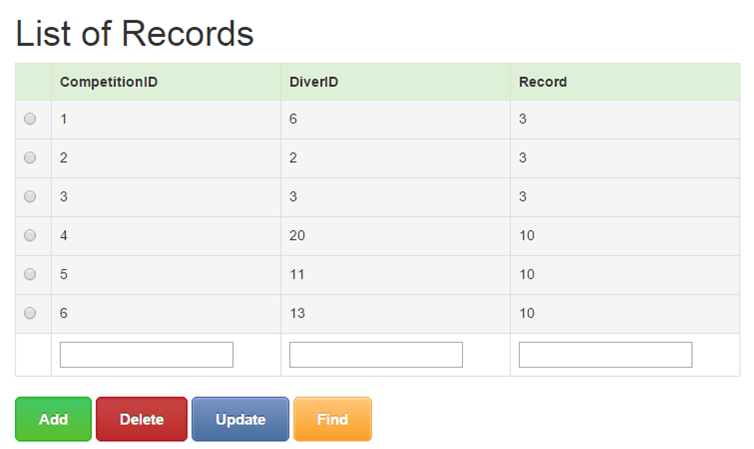
\includegraphics{recordtable.png}}
\caption{Fig. 1.3: Screenshot of Record Table}\end{figure}

Information about record is listed on the screen.
Data table consist of competitionID, DiverID and record.
CompetitionID is the unique ID of the competition.
DiverID is the unique ID of the sporter.
Record is the amount of height sporter dived from.

Operations add, delete, update and find can be done from this section alone.
The sporter with the ID number DiverID and competition with the CompetitionID must exist in order to add a new record.


\chapter{Developer Guide}
\label{developer/index::doc}\label{developer/index:developer-guide}

\section{Database Design}
\label{developer/index:database-design}
\textbf{explain the database design of your project}

\textbf{include the E/R diagram(s)}


\section{Code}
\label{developer/index:code}
\textbf{explain the technical structure of your code}

\textbf{to include a code listing, use the following example}:

\begin{Verbatim}[commandchars=\\\{\}]
.. code\PYGZhy{}block:: python

   class Foo:

      def \PYGZus{}\PYGZus{}init\PYGZus{}\PYGZus{}(self, x):
         self.x = x
\end{Verbatim}


\subsection{Parts Implemented by Member Name}
\label{developer/member1:parts-implemented-by-member-name}\label{developer/member1::doc}

\subsection{Parts Implemented by Cemal Türkoğlu}
\label{developer/member2::doc}\label{developer/member2:parts-implemented-by-cemal-turkoglu}

\subsubsection{Statistics Operations}
\label{developer/member2:statistics-operations}
The power boat racing page supply some statistics for user .
\begin{quote}

\scalebox{1.000000}{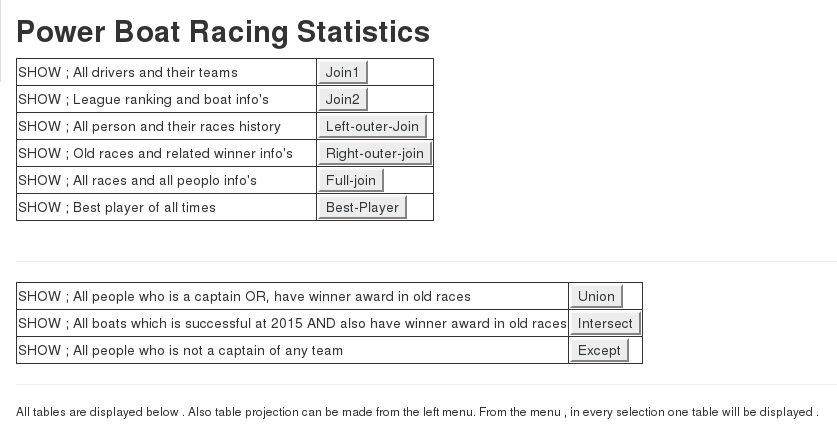
\includegraphics{statistic.png}}
\end{quote}


\paragraph{All Drivers And Their Teams}
\label{developer/member2:all-drivers-and-their-teams}\begin{quote}

\scalebox{1.000000}{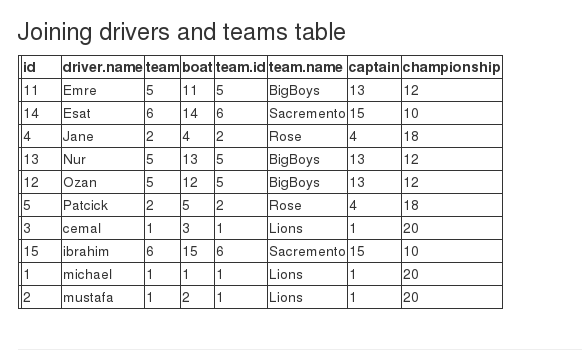
\includegraphics{join1.png}}
\end{quote}

The code:
\begin{quote}

\scalebox{1.000000}{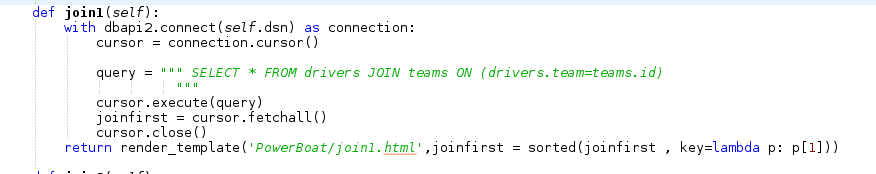
\includegraphics{join1c.png}}
\end{quote}


\paragraph{League ranking and boat info's}
\label{developer/member2:league-ranking-and-boat-info-s}\begin{quote}

\scalebox{1.000000}{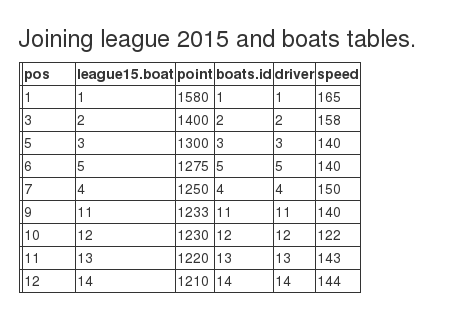
\includegraphics{join2.png}}
\end{quote}

The code:
\begin{quote}

\scalebox{1.000000}{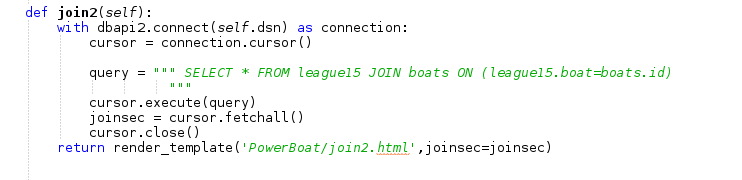
\includegraphics{join2c.png}}
\end{quote}


\paragraph{All person and their races history}
\label{developer/member2:all-person-and-their-races-history}\begin{quote}

\scalebox{1.000000}{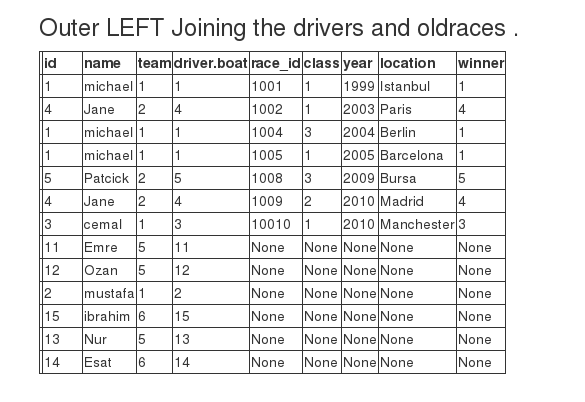
\includegraphics{leftj.png}}
\end{quote}

The code:
\begin{quote}

\scalebox{1.000000}{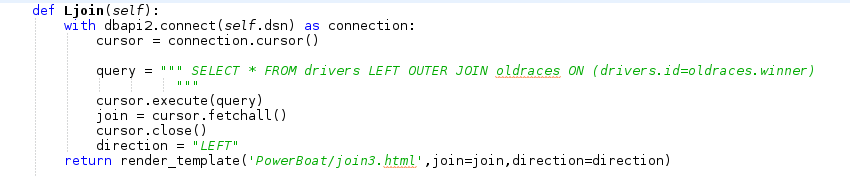
\includegraphics{leftjc.png}}
\end{quote}


\paragraph{Old races and related winner info's}
\label{developer/member2:old-races-and-related-winner-info-s}\begin{quote}

\scalebox{1.000000}{\includegraphics{developer/images/cemal/rigthj.png}}
\end{quote}

The code:
\begin{quote}

\scalebox{1.000000}{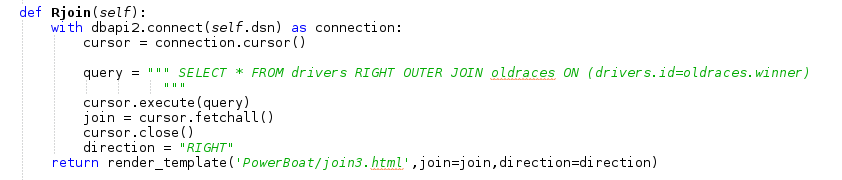
\includegraphics{rightjc.png}}
\end{quote}


\paragraph{All races and all peoplo info's}
\label{developer/member2:all-races-and-all-peoplo-info-s}\begin{quote}

\scalebox{1.000000}{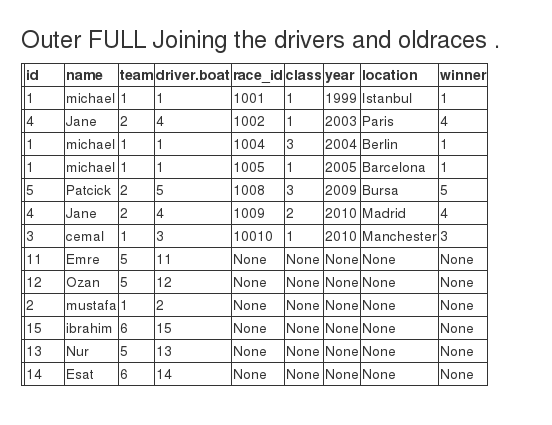
\includegraphics{fullj.png}}
\end{quote}

The code:
\begin{quote}

\scalebox{1.000000}{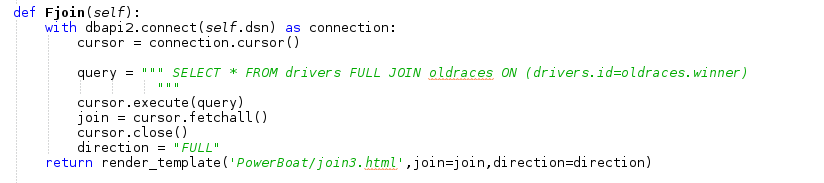
\includegraphics{fulljc.png}}
\end{quote}


\paragraph{Best player of all times}
\label{developer/member2:best-player-of-all-times}\begin{quote}

\scalebox{1.000000}{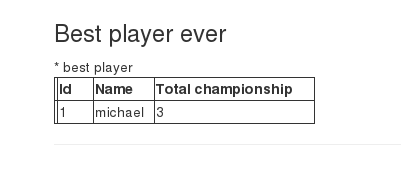
\includegraphics{best.png}}
\end{quote}

The code:
\begin{quote}

\scalebox{1.000000}{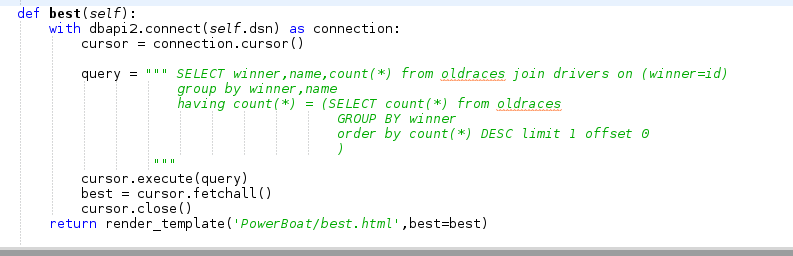
\includegraphics{bestc.png}}
\end{quote}


\paragraph{All people who is a captain OR, have winner award in old races}
\label{developer/member2:all-people-who-is-a-captain-or-have-winner-award-in-old-races}\begin{quote}

\scalebox{1.000000}{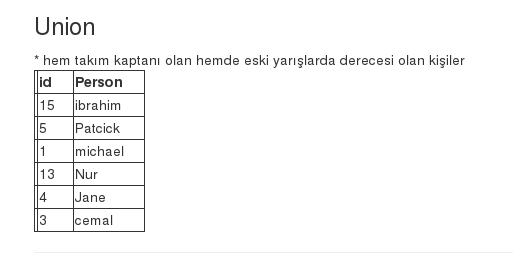
\includegraphics{union.png}}
\end{quote}

The code:
\begin{quote}

\scalebox{1.000000}{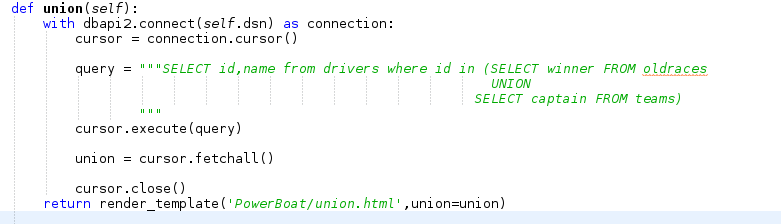
\includegraphics{unionc.png}}
\end{quote}


\paragraph{All boats which is successful at 2015 AND also have winner award in old races}
\label{developer/member2:all-boats-which-is-successful-at-2015-and-also-have-winner-award-in-old-races}\begin{quote}

\scalebox{1.000000}{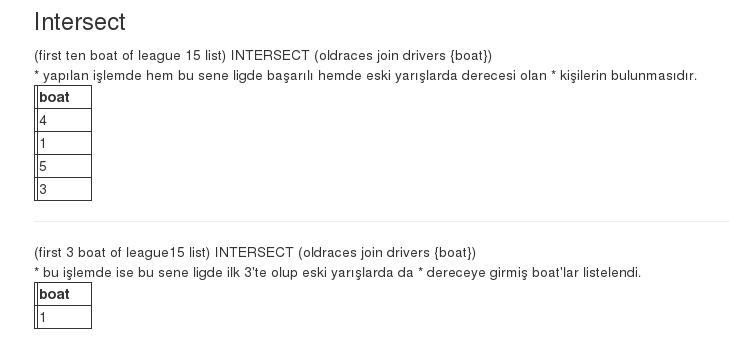
\includegraphics{intersect.png}}
\end{quote}

The code:
\begin{quote}

\scalebox{1.000000}{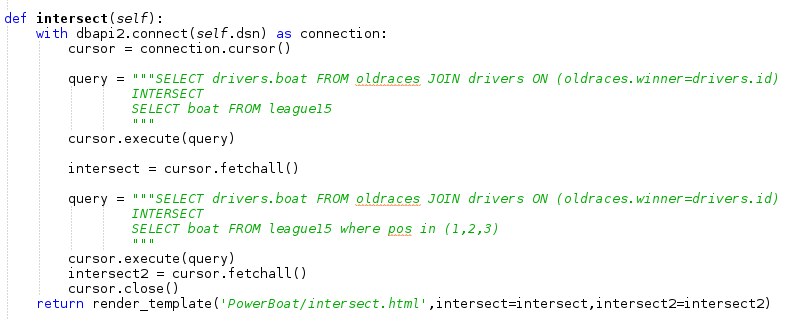
\includegraphics{intersectc.png}}
\end{quote}


\paragraph{All people who is not a captain of any team}
\label{developer/member2:all-people-who-is-not-a-captain-of-any-team}\begin{quote}

\scalebox{1.000000}{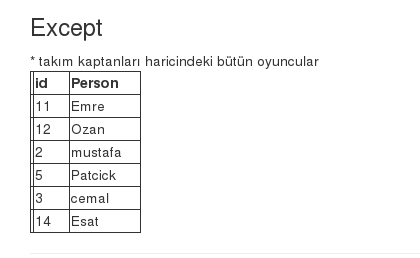
\includegraphics{except.png}}
\end{quote}

The code:
\begin{quote}

\scalebox{1.000000}{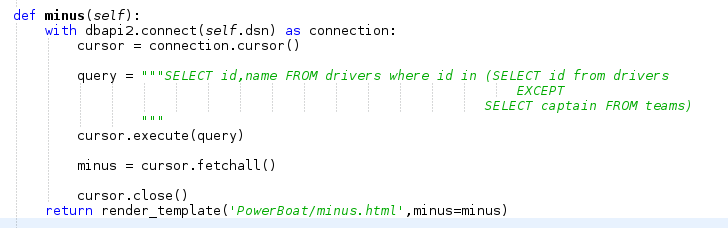
\includegraphics{exceptc.png}}
\end{quote}


\subsection{Parts Implemented by Member Name}
\label{developer/member3:parts-implemented-by-member-name}\label{developer/member3::doc}

\subsection{Parts Implemented by Ercan Alp Serteli}
\label{developer/member4:parts-implemented-by-ercan-alp-serteli}\label{developer/member4::doc}
I have implemented three database tables: competitors, teams and users. The first two tables are regarding the Underwater Photography and they are managed by the \emph{UWP} class. The users table is managed by the \emph{Users} class.

Here, I will explain everything technical that is related to these entities including SQL code, Python code and HTML code.


\subsubsection{UWP Class}
\label{developer/member4:uwp-class}
The \emph{UWP} class includes all the methods that are needed to manage the \emph{competitor} and \emph{team} tables


\paragraph{init Method}
\label{developer/member4:init-method}\begin{quote}

\begin{Verbatim}[commandchars=\\\{\}]
\PYG{k}{def} \PYG{n+nf}{\PYGZus{}\PYGZus{}init\PYGZus{}\PYGZus{}}\PYG{p}{(}\PYG{n+nb+bp}{self}\PYG{p}{,} \PYG{n}{dsn}\PYG{p}{)}\PYG{p}{:}
  \PYG{n+nb+bp}{self}\PYG{o}{.}\PYG{n}{dsn} \PYG{o}{=} \PYG{n}{dsn}
  \PYG{k}{with} \PYG{n}{dbapi2}\PYG{o}{.}\PYG{n}{connect}\PYG{p}{(}\PYG{n+nb+bp}{self}\PYG{o}{.}\PYG{n}{dsn}\PYG{p}{)} \PYG{k}{as} \PYG{n}{connection}\PYG{p}{:}
      \PYG{n}{cursor} \PYG{o}{=} \PYG{n}{connection}\PYG{o}{.}\PYG{n}{cursor}\PYG{p}{(}\PYG{p}{)}
      \PYG{n}{query} \PYG{o}{=}  \PYG{l+s}{\PYGZdq{}\PYGZdq{}\PYGZdq{}}\PYG{l+s}{DO \PYGZdl{}\PYGZdl{}}
\PYG{l+s}{                  BEGIN}
\PYG{l+s}{                      IF NOT EXISTS (SELECT 1 FROM pg\PYGZus{}type WHERE typname = }\PYG{l+s}{\PYGZsq{}}\PYG{l+s}{role}\PYG{l+s}{\PYGZsq{}}\PYG{l+s}{) THEN}
\PYG{l+s}{                          CREATE TYPE role AS ENUM (}\PYG{l+s}{\PYGZsq{}}\PYG{l+s}{Photographer}\PYG{l+s}{\PYGZsq{}}\PYG{l+s}{, }\PYG{l+s}{\PYGZsq{}}\PYG{l+s}{Assistant}\PYG{l+s}{\PYGZsq{}}\PYG{l+s}{, }\PYG{l+s}{\PYGZsq{}}\PYG{l+s}{Captain}\PYG{l+s}{\PYGZsq{}}\PYG{l+s}{);}
\PYG{l+s}{                      END IF;}
\PYG{l+s}{                  END\PYGZdl{}\PYGZdl{}}\PYG{l+s}{\PYGZdq{}\PYGZdq{}\PYGZdq{}}
      \PYG{n}{cursor}\PYG{o}{.}\PYG{n}{execute}\PYG{p}{(}\PYG{n}{query}\PYG{p}{)}

      \PYG{n}{query} \PYG{o}{=} \PYG{l+s}{\PYGZdq{}\PYGZdq{}\PYGZdq{}}\PYG{l+s}{CREATE TABLE IF NOT EXISTS team (}
\PYG{l+s}{                  id serial PRIMARY KEY,}
\PYG{l+s}{                  country text NOT NULL)}\PYG{l+s}{\PYGZdq{}\PYGZdq{}\PYGZdq{}}
      \PYG{n}{cursor}\PYG{o}{.}\PYG{n}{execute}\PYG{p}{(}\PYG{n}{query}\PYG{p}{)}

      \PYG{n}{query} \PYG{o}{=} \PYG{l+s}{\PYGZdq{}\PYGZdq{}\PYGZdq{}}\PYG{l+s}{CREATE TABLE IF NOT EXISTS competitor (}
\PYG{l+s}{                  id serial PRIMARY KEY,}
\PYG{l+s}{                  name text NOT NULL,}
\PYG{l+s}{                  surname text NOT NULL,}
\PYG{l+s}{                  role role NOT NULL,}
\PYG{l+s}{                  team\PYGZus{}id integer REFERENCES team (id))}\PYG{l+s}{\PYGZdq{}\PYGZdq{}\PYGZdq{}}
      \PYG{n}{cursor}\PYG{o}{.}\PYG{n}{execute}\PYG{p}{(}\PYG{n}{query}\PYG{p}{)}
  \PYG{k}{return}
\end{Verbatim}
\end{quote}

This is the method that gets called when the UWP object is created. It gets the dsn by a parameter and saves it in its field for later use. Then it attempts to create the role type and the two tables if they do not exist. These SQL statements do nothing if the database has been initialized properly. They are there in case the application might be needed to run in a new database or some of the tables are dropped for some reason.


\paragraph{show\_page\_comp Method}
\label{developer/member4:show-page-comp-method}\begin{quote}

\begin{Verbatim}[commandchars=\\\{\}]
\PYG{k}{def} \PYG{n+nf}{show\PYGZus{}page\PYGZus{}comp}\PYG{p}{(}\PYG{n+nb+bp}{self}\PYG{p}{)}\PYG{p}{:}
  \PYG{k}{with} \PYG{n}{dbapi2}\PYG{o}{.}\PYG{n}{connect}\PYG{p}{(}\PYG{n+nb+bp}{self}\PYG{o}{.}\PYG{n}{dsn}\PYG{p}{)} \PYG{k}{as} \PYG{n}{connection}\PYG{p}{:}
      \PYG{n}{cursor} \PYG{o}{=} \PYG{n}{connection}\PYG{o}{.}\PYG{n}{cursor}\PYG{p}{(}\PYG{p}{)}

      \PYG{n}{query} \PYG{o}{=} \PYG{l+s}{\PYGZdq{}\PYGZdq{}\PYGZdq{}}\PYG{l+s}{SELECT competitor.id, name, surname, country, role FROM competitor, team}
\PYG{l+s}{                  WHERE (team\PYGZus{}id = team.id)}\PYG{l+s}{\PYGZdq{}\PYGZdq{}\PYGZdq{}}
      \PYG{n}{cursor}\PYG{o}{.}\PYG{n}{execute}\PYG{p}{(}\PYG{n}{query}\PYG{p}{)}
      \PYG{n}{competitors} \PYG{o}{=} \PYG{n}{cursor}\PYG{o}{.}\PYG{n}{fetchall}\PYG{p}{(}\PYG{p}{)}

      \PYG{n}{query} \PYG{o}{=} \PYG{l+s}{\PYGZdq{}}\PYG{l+s}{SELECT country FROM team}\PYG{l+s}{\PYGZdq{}}
      \PYG{n}{cursor}\PYG{o}{.}\PYG{n}{execute}\PYG{p}{(}\PYG{n}{query}\PYG{p}{)}
      \PYG{n}{countries} \PYG{o}{=} \PYG{p}{[}\PYG{p}{]}
      \PYG{k}{for} \PYG{n}{row} \PYG{o+ow}{in} \PYG{n}{cursor}\PYG{p}{:}
          \PYG{n}{countries}\PYG{o}{.}\PYG{n}{append}\PYG{p}{(}\PYG{n}{row}\PYG{p}{[}\PYG{l+m+mi}{0}\PYG{p}{]}\PYG{p}{)}
      \PYG{n}{query} \PYG{o}{=} \PYG{l+s}{\PYGZdq{}}\PYG{l+s}{SELECT DISTINCT role FROM competitor}\PYG{l+s}{\PYGZdq{}}
      \PYG{n}{cursor}\PYG{o}{.}\PYG{n}{execute}\PYG{p}{(}\PYG{n}{query}\PYG{p}{)}
      \PYG{n}{roles} \PYG{o}{=} \PYG{p}{[}\PYG{p}{]}
      \PYG{k}{for} \PYG{n}{row} \PYG{o+ow}{in} \PYG{n}{cursor}\PYG{p}{:}
          \PYG{n}{roles}\PYG{o}{.}\PYG{n}{append}\PYG{p}{(}\PYG{n}{row}\PYG{p}{[}\PYG{l+m+mi}{0}\PYG{p}{]}\PYG{p}{)}

  \PYG{k}{return} \PYG{n}{render\PYGZus{}template}\PYG{p}{(}\PYG{l+s}{\PYGZsq{}}\PYG{l+s}{uwp/uwp\PYGZus{}comp.html}\PYG{l+s}{\PYGZsq{}}\PYG{p}{,} \PYG{n}{competitors} \PYG{o}{=} \PYG{n+nb}{sorted}\PYG{p}{(}\PYG{n}{competitors}\PYG{p}{,} \PYG{n}{key}\PYG{o}{=}\PYG{k}{lambda} \PYG{n}{p}\PYG{p}{:} \PYG{n}{p}\PYG{p}{[}\PYG{l+m+mi}{1}\PYG{p}{]}\PYG{p}{)}\PYG{p}{,}
                         \PYG{n}{countries} \PYG{o}{=} \PYG{n}{countries}\PYG{p}{,} \PYG{n}{roles} \PYG{o}{=} \PYG{n}{roles}\PYG{p}{)}
\end{Verbatim}
\end{quote}

This method is called when a HTTP GET is requested for the competitors page. It gets the data that is needed to construct the competitor list from the database and renders the page with that data as the parameter. It sorts the list by the first names before using it.
In the first select statement, we get the data of all competitors by joining the competitor and team tables over team\_id. This way, we can display the countries that each competitor belongs to as well as their other attributes.
The second select statement is used to get all the countries from the team table so that they can be shown in a dropdown menu when adding or updating rows.
The last select statement gets the roles that are used in the competitor table for a dropdown menu again. I just noticed that this is a very bad way of doing this. It should get them from the type instead of the table. However it is too late to fix this now.


\paragraph{show\_page\_team Method}
\label{developer/member4:show-page-team-method}\begin{quote}

\begin{Verbatim}[commandchars=\\\{\}]
\PYG{k}{def} \PYG{n+nf}{show\PYGZus{}page\PYGZus{}team}\PYG{p}{(}\PYG{n+nb+bp}{self}\PYG{p}{)}\PYG{p}{:}
  \PYG{k}{with} \PYG{n}{dbapi2}\PYG{o}{.}\PYG{n}{connect}\PYG{p}{(}\PYG{n+nb+bp}{self}\PYG{o}{.}\PYG{n}{dsn}\PYG{p}{)} \PYG{k}{as} \PYG{n}{connection}\PYG{p}{:}
      \PYG{n}{cursor} \PYG{o}{=} \PYG{n}{connection}\PYG{o}{.}\PYG{n}{cursor}\PYG{p}{(}\PYG{p}{)}

      \PYG{n}{query} \PYG{o}{=} \PYG{l+s}{\PYGZdq{}\PYGZdq{}\PYGZdq{}}\PYG{l+s}{SELECT team.id, country, COUNT(competitor.id)}
\PYG{l+s}{                  FROM team LEFT JOIN competitor  ON team\PYGZus{}id = team.id}
\PYG{l+s}{                  GROUP BY team.id}\PYG{l+s}{\PYGZdq{}\PYGZdq{}\PYGZdq{}}

      \PYG{n}{cursor}\PYG{o}{.}\PYG{n}{execute}\PYG{p}{(}\PYG{n}{query}\PYG{p}{)}
      \PYG{n}{teams} \PYG{o}{=} \PYG{n}{cursor}\PYG{o}{.}\PYG{n}{fetchall}\PYG{p}{(}\PYG{p}{)}

  \PYG{k}{return} \PYG{n}{render\PYGZus{}template}\PYG{p}{(}\PYG{l+s}{\PYGZsq{}}\PYG{l+s}{uwp/uwp\PYGZus{}teams.html}\PYG{l+s}{\PYGZsq{}}\PYG{p}{,} \PYG{n}{teams} \PYG{o}{=} \PYG{n}{teams}\PYG{p}{)}
\end{Verbatim}
\end{quote}

This method is for showing the teams page. It gets the team data and the number of competitors in each team by joining the team and competitor tables. Left join is used because we want to get all the teams in the list whether they have any members or not.


\paragraph{add\_competitor Method}
\label{developer/member4:add-competitor-method}\begin{quote}

\begin{Verbatim}[commandchars=\\\{\}]
\PYG{n}{query} \PYG{o}{=} \PYG{l+s}{\PYGZdq{}\PYGZdq{}\PYGZdq{}}\PYG{l+s}{INSERT INTO competitor (name, surname, role, team\PYGZus{}id)}
\PYG{l+s}{               SELECT }\PYG{l+s+si}{\PYGZpc{}s}\PYG{l+s}{, }\PYG{l+s+si}{\PYGZpc{}s}\PYG{l+s}{, }\PYG{l+s+si}{\PYGZpc{}s}\PYG{l+s}{, team.id}
\PYG{l+s}{               FROM team WHERE team.country = }\PYG{l+s+si}{\PYGZpc{}s}
\PYG{l+s}{               }\PYG{l+s}{\PYGZdq{}\PYGZdq{}\PYGZdq{}}
\PYG{n}{cursor}\PYG{o}{.}\PYG{n}{execute}\PYG{p}{(}\PYG{n}{query}\PYG{p}{,} \PYG{p}{(}\PYG{n}{name}\PYG{p}{,} \PYG{n}{surname}\PYG{p}{,} \PYG{n}{role}\PYG{p}{,} \PYG{n}{country}\PYG{p}{)}\PYG{p}{)}
\end{Verbatim}

\begin{notice}{note}{Note:}
From now on, in most methods only a relevant part of the method is pasted
\end{notice}
\end{quote}

This method is used to insert a row into the competitor table. The team\_id needed is selected from team using the country.


\paragraph{delete\_competitor Method}
\label{developer/member4:delete-competitor-method}\begin{quote}

\begin{Verbatim}[commandchars=\\\{\}]
\PYG{n}{query} \PYG{o}{=} \PYG{l+s}{\PYGZdq{}}\PYG{l+s}{DELETE FROM competitor WHERE id = }\PYG{l+s+si}{\PYGZpc{}s}\PYG{l+s}{\PYGZdq{}}
\PYG{n}{cursor}\PYG{o}{.}\PYG{n}{execute}\PYG{p}{(}\PYG{n}{query}\PYG{p}{,} \PYG{p}{(}\PYG{n+nb}{id}\PYG{p}{,}\PYG{p}{)}\PYG{p}{)}
\end{Verbatim}
\end{quote}

This is a very simple method as it only gets an id and deletes the row with that id from the table.


\paragraph{update\_competitor Method}
\label{developer/member4:update-competitor-method}\begin{quote}

\begin{Verbatim}[commandchars=\\\{\}]
\PYG{n}{query} \PYG{o}{=} \PYG{l+s}{\PYGZdq{}\PYGZdq{}\PYGZdq{}}\PYG{l+s}{UPDATE competitor}
\PYG{l+s}{         SET name=}\PYG{l+s+si}{\PYGZpc{}s}\PYG{l+s}{,surname=}\PYG{l+s+si}{\PYGZpc{}s}\PYG{l+s}{,role=}\PYG{l+s+si}{\PYGZpc{}s}\PYG{l+s}{,team\PYGZus{}id=subquery.id}
\PYG{l+s}{         FROM (SELECT team.id FROM team WHERE team.country = }\PYG{l+s+si}{\PYGZpc{}s}\PYG{l+s}{)}
\PYG{l+s}{         AS subquery}
\PYG{l+s}{         WHERE competitor.id = }\PYG{l+s+si}{\PYGZpc{}s}\PYG{l+s}{\PYGZdq{}\PYGZdq{}\PYGZdq{}}
\PYG{n}{cursor}\PYG{o}{.}\PYG{n}{execute}\PYG{p}{(}\PYG{n}{query}\PYG{p}{,} \PYG{p}{(}\PYG{n}{name}\PYG{p}{,} \PYG{n}{surname}\PYG{p}{,} \PYG{n}{role}\PYG{p}{,} \PYG{n}{country}\PYG{p}{,} \PYG{n+nb}{id}\PYG{p}{)}\PYG{p}{)}
\end{Verbatim}
\end{quote}

This method updates a row in the competitor table with the new data. It uses the name, surname and role inputs directly while it gets the team\_id using a subquery that uses the country input.


\paragraph{add\_team Method}
\label{developer/member4:add-team-method}\begin{quote}

\begin{Verbatim}[commandchars=\\\{\}]
\PYG{n}{query} \PYG{o}{=} \PYG{l+s}{\PYGZdq{}\PYGZdq{}\PYGZdq{}}\PYG{l+s}{INSERT INTO team (country)}
\PYG{l+s}{         VALUES (}\PYG{l+s+si}{\PYGZpc{}s}\PYG{l+s}{)}\PYG{l+s}{\PYGZdq{}\PYGZdq{}\PYGZdq{}}
\PYG{n}{cursor}\PYG{o}{.}\PYG{n}{execute}\PYG{p}{(}\PYG{n}{query}\PYG{p}{,} \PYG{p}{(}\PYG{n}{country}\PYG{p}{,}\PYG{p}{)}\PYG{p}{)}
\end{Verbatim}
\end{quote}

Self explanatory method that adds a new row to the team table.


\paragraph{update\_team Method}
\label{developer/member4:update-team-method}\begin{quote}

\begin{Verbatim}[commandchars=\\\{\}]
\PYG{n}{query} \PYG{o}{=} \PYG{l+s}{\PYGZdq{}\PYGZdq{}\PYGZdq{}}\PYG{l+s}{UPDATE team}
\PYG{l+s}{            SET country = }\PYG{l+s+si}{\PYGZpc{}s}
\PYG{l+s}{            WHERE id = }\PYG{l+s+si}{\PYGZpc{}s}\PYG{l+s}{\PYGZdq{}\PYGZdq{}\PYGZdq{}}
\PYG{n}{cursor}\PYG{o}{.}\PYG{n}{execute}\PYG{p}{(}\PYG{n}{query}\PYG{p}{,} \PYG{p}{(}\PYG{n}{country}\PYG{p}{,} \PYG{n+nb}{id}\PYG{p}{)}\PYG{p}{)}
\end{Verbatim}
\end{quote}

Self explanatory method that updates new row in the team table.


\paragraph{delete\_team Method}
\label{developer/member4:delete-team-method}\begin{quote}

\begin{Verbatim}[commandchars=\\\{\}]
\PYG{n}{query} \PYG{o}{=} \PYG{l+s}{\PYGZdq{}\PYGZdq{}\PYGZdq{}}\PYG{l+s}{SELECT team.id, country, COUNT(competitor.id)}
\PYG{l+s}{            FROM team LEFT JOIN competitor  ON team\PYGZus{}id = team.id}
\PYG{l+s}{            WHERE team.id = }\PYG{l+s+si}{\PYGZpc{}s}\PYG{l+s}{ GROUP BY team.id}
\PYG{l+s}{            }\PYG{l+s}{\PYGZdq{}\PYGZdq{}\PYGZdq{}}
\PYG{n}{cursor}\PYG{o}{.}\PYG{n}{execute}\PYG{p}{(}\PYG{n}{query}\PYG{p}{,} \PYG{p}{(}\PYG{n+nb}{id}\PYG{p}{,}\PYG{p}{)}\PYG{p}{)}
\PYG{n+nb}{id}\PYG{p}{,} \PYG{n}{country}\PYG{p}{,} \PYG{n}{members} \PYG{o}{=} \PYG{n}{cursor}\PYG{o}{.}\PYG{n}{fetchone}\PYG{p}{(}\PYG{p}{)}

\PYG{k}{if} \PYG{n}{members} \PYG{o}{!=} \PYG{l+m+mi}{0}\PYG{p}{:}
    \PYG{n}{flash}\PYG{p}{(}\PYG{l+s}{\PYGZdq{}}\PYG{l+s}{You cannot delete a team that has members in the competitor list!}\PYG{l+s}{\PYGZdq{}}\PYG{p}{)}
\PYG{k}{else}\PYG{p}{:}
    \PYG{n}{query} \PYG{o}{=} \PYG{l+s}{\PYGZdq{}}\PYG{l+s}{DELETE FROM team WHERE id = }\PYG{l+s+si}{\PYGZpc{}s}\PYG{l+s}{\PYGZdq{}}
    \PYG{n}{cursor}\PYG{o}{.}\PYG{n}{execute}\PYG{p}{(}\PYG{n}{query}\PYG{p}{,} \PYG{p}{(}\PYG{n+nb}{id}\PYG{p}{,}\PYG{p}{)}\PYG{p}{)}
\end{Verbatim}
\end{quote}

This method is used for deleting a row from the team table. However, it has to check if there are any members of the team before attempting to delete it. So, it gets the number of members in a team in the same way show\_page\_team does. Then checks if the number is 0. If it is, then it is deleted. Otherwise, it pops a flash message and reloads the page.


\paragraph{reset\_table Method}
\label{developer/member4:reset-table-method}\begin{quote}

\begin{Verbatim}[commandchars=\\\{\}]
\PYG{n}{query} \PYG{o}{=} \PYG{l+s}{\PYGZdq{}\PYGZdq{}\PYGZdq{}}\PYG{l+s}{DROP TABLE IF EXISTS competitor;}
\PYG{l+s}{            DROP TABLE IF EXISTS team;}
\PYG{l+s}{            DROP TYPE IF EXISTS role;}\PYG{l+s}{\PYGZdq{}\PYGZdq{}\PYGZdq{}}
\PYG{n}{cursor}\PYG{o}{.}\PYG{n}{execute}\PYG{p}{(}\PYG{n}{query}\PYG{p}{)}

\PYG{n}{query} \PYG{o}{=} \PYG{l+s}{\PYGZdq{}}\PYG{l+s}{CREATE TYPE role AS ENUM (}\PYG{l+s}{\PYGZsq{}}\PYG{l+s}{Photographer}\PYG{l+s}{\PYGZsq{}}\PYG{l+s}{, }\PYG{l+s}{\PYGZsq{}}\PYG{l+s}{Assistant}\PYG{l+s}{\PYGZsq{}}\PYG{l+s}{, }\PYG{l+s}{\PYGZsq{}}\PYG{l+s}{Captain}\PYG{l+s}{\PYGZsq{}}\PYG{l+s}{)}\PYG{l+s}{\PYGZdq{}}
\PYG{n}{cursor}\PYG{o}{.}\PYG{n}{execute}\PYG{p}{(}\PYG{n}{query}\PYG{p}{)}

\PYG{n}{query} \PYG{o}{=} \PYG{l+s}{\PYGZdq{}\PYGZdq{}\PYGZdq{}}\PYG{l+s}{CREATE TABLE team (}
\PYG{l+s}{            id serial PRIMARY KEY,}
\PYG{l+s}{            country text NOT NULL)}\PYG{l+s}{\PYGZdq{}\PYGZdq{}\PYGZdq{}}
\PYG{n}{cursor}\PYG{o}{.}\PYG{n}{execute}\PYG{p}{(}\PYG{n}{query}\PYG{p}{)}

\PYG{n}{query} \PYG{o}{=} \PYG{l+s}{\PYGZdq{}\PYGZdq{}\PYGZdq{}}\PYG{l+s}{CREATE TABLE competitor (}
\PYG{l+s}{            id serial PRIMARY KEY,}
\PYG{l+s}{            name text NOT NULL,}
\PYG{l+s}{            surname text NOT NULL,}
\PYG{l+s}{            role role NOT NULL,}
\PYG{l+s}{            team\PYGZus{}id integer REFERENCES team (id))}\PYG{l+s}{\PYGZdq{}\PYGZdq{}\PYGZdq{}}
\PYG{n}{cursor}\PYG{o}{.}\PYG{n}{execute}\PYG{p}{(}\PYG{n}{query}\PYG{p}{)}

\PYG{n}{query} \PYG{o}{=} \PYG{l+s}{\PYGZdq{}\PYGZdq{}\PYGZdq{}}\PYG{l+s}{INSERT INTO team (country)}
\PYG{l+s}{            VALUES}
\PYG{l+s}{            (}\PYG{l+s}{\PYGZsq{}}\PYG{l+s}{Turkey}\PYG{l+s}{\PYGZsq{}}\PYG{l+s}{),}
\PYG{l+s}{            (}\PYG{l+s}{\PYGZsq{}}\PYG{l+s}{Italy}\PYG{l+s}{\PYGZsq{}}\PYG{l+s}{)}
\PYG{l+s}{            }\PYG{l+s}{\PYGZdq{}\PYGZdq{}\PYGZdq{}}
\PYG{n}{cursor}\PYG{o}{.}\PYG{n}{execute}\PYG{p}{(}\PYG{n}{query}\PYG{p}{)}

\PYG{n}{query} \PYG{o}{=} \PYG{l+s}{\PYGZdq{}\PYGZdq{}\PYGZdq{}}\PYG{l+s}{INSERT INTO competitor (name, surname, role, team\PYGZus{}id)}
\PYG{l+s}{            VALUES}
\PYG{l+s}{            (}\PYG{l+s}{\PYGZsq{}}\PYG{l+s}{Ahmet}\PYG{l+s}{\PYGZsq{}}\PYG{l+s}{, }\PYG{l+s}{\PYGZsq{}}\PYG{l+s}{KARPUZSEVER}\PYG{l+s}{\PYGZsq{}}\PYG{l+s}{, }\PYG{l+s}{\PYGZsq{}}\PYG{l+s}{Photographer}\PYG{l+s}{\PYGZsq{}}\PYG{l+s}{, 1),}
\PYG{l+s}{            (}\PYG{l+s}{\PYGZsq{}}\PYG{l+s}{Orhan}\PYG{l+s}{\PYGZsq{}}\PYG{l+s}{, }\PYG{l+s}{\PYGZsq{}}\PYG{l+s}{AYTUR}\PYG{l+s}{\PYGZsq{}}\PYG{l+s}{, }\PYG{l+s}{\PYGZsq{}}\PYG{l+s}{Captain}\PYG{l+s}{\PYGZsq{}}\PYG{l+s}{, 1),}
\PYG{l+s}{            (}\PYG{l+s}{\PYGZsq{}}\PYG{l+s}{Melek}\PYG{l+s}{\PYGZsq{}}\PYG{l+s}{, }\PYG{l+s}{\PYGZsq{}}\PYG{l+s}{KOYUKANAT}\PYG{l+s}{\PYGZsq{}}\PYG{l+s}{, }\PYG{l+s}{\PYGZsq{}}\PYG{l+s}{Photographer}\PYG{l+s}{\PYGZsq{}}\PYG{l+s}{, 1),}
\PYG{l+s}{            (}\PYG{l+s}{\PYGZsq{}}\PYG{l+s}{Leyla}\PYG{l+s}{\PYGZsq{}}\PYG{l+s}{, }\PYG{l+s}{\PYGZsq{}}\PYG{l+s}{LALECI}\PYG{l+s}{\PYGZsq{}}\PYG{l+s}{, }\PYG{l+s}{\PYGZsq{}}\PYG{l+s}{Assistant}\PYG{l+s}{\PYGZsq{}}\PYG{l+s}{, 1),}
\PYG{l+s}{            (}\PYG{l+s}{\PYGZsq{}}\PYG{l+s}{Ivo}\PYG{l+s}{\PYGZsq{}}\PYG{l+s}{, }\PYG{l+s}{\PYGZsq{}}\PYG{l+s}{MONALDO}\PYG{l+s}{\PYGZsq{}}\PYG{l+s}{, }\PYG{l+s}{\PYGZsq{}}\PYG{l+s}{Photographer}\PYG{l+s}{\PYGZsq{}}\PYG{l+s}{, 2),}
\PYG{l+s}{            (}\PYG{l+s}{\PYGZsq{}}\PYG{l+s}{Rosita}\PYG{l+s}{\PYGZsq{}}\PYG{l+s}{, }\PYG{l+s}{\PYGZsq{}}\PYG{l+s}{BUCCHO}\PYG{l+s}{\PYGZsq{}}\PYG{l+s}{, }\PYG{l+s}{\PYGZsq{}}\PYG{l+s}{Assistant}\PYG{l+s}{\PYGZsq{}}\PYG{l+s}{, 2),}
\PYG{l+s}{            (}\PYG{l+s}{\PYGZsq{}}\PYG{l+s}{Callan}\PYG{l+s}{\PYGZsq{}}\PYG{l+s}{, }\PYG{l+s}{\PYGZsq{}}\PYG{l+s}{ROBERTSON}\PYG{l+s}{\PYGZsq{}}\PYG{l+s}{, }\PYG{l+s}{\PYGZsq{}}\PYG{l+s}{Assistant}\PYG{l+s}{\PYGZsq{}}\PYG{l+s}{, 2),}
\PYG{l+s}{            (}\PYG{l+s}{\PYGZsq{}}\PYG{l+s}{Katarina}\PYG{l+s}{\PYGZsq{}}\PYG{l+s}{, }\PYG{l+s}{\PYGZsq{}}\PYG{l+s}{LONCAR}\PYG{l+s}{\PYGZsq{}}\PYG{l+s}{, }\PYG{l+s}{\PYGZsq{}}\PYG{l+s}{Captain}\PYG{l+s}{\PYGZsq{}}\PYG{l+s}{, 2),}
\PYG{l+s}{            (}\PYG{l+s}{\PYGZsq{}}\PYG{l+s}{Fastred}\PYG{l+s}{\PYGZsq{}}\PYG{l+s}{, }\PYG{l+s}{\PYGZsq{}}\PYG{l+s}{RUMBLE}\PYG{l+s}{\PYGZsq{}}\PYG{l+s}{, }\PYG{l+s}{\PYGZsq{}}\PYG{l+s}{Photographer}\PYG{l+s}{\PYGZsq{}}\PYG{l+s}{, 2)}
\PYG{l+s}{            }\PYG{l+s}{\PYGZdq{}\PYGZdq{}\PYGZdq{}}
\PYG{n}{cursor}\PYG{o}{.}\PYG{n}{execute}\PYG{p}{(}\PYG{n}{query}\PYG{p}{)}
\end{Verbatim}
\end{quote}

This method drops the team and competitor tables, creates them again and fills them with default data.


\subsubsection{Users Class}
\label{developer/member4:users-class}
This class has all the methods that are needed for managing the users table.


\paragraph{init Method}
\label{developer/member4:id1}\begin{quote}

\begin{Verbatim}[commandchars=\\\{\}]
\PYG{k}{def} \PYG{n+nf}{\PYGZus{}\PYGZus{}init\PYGZus{}\PYGZus{}}\PYG{p}{(}\PYG{n+nb+bp}{self}\PYG{p}{,} \PYG{n}{dsn}\PYG{p}{)}\PYG{p}{:}
  \PYG{n+nb+bp}{self}\PYG{o}{.}\PYG{n}{dsn} \PYG{o}{=} \PYG{n}{dsn}
  \PYG{k}{with} \PYG{n}{dbapi2}\PYG{o}{.}\PYG{n}{connect}\PYG{p}{(}\PYG{n+nb+bp}{self}\PYG{o}{.}\PYG{n}{dsn}\PYG{p}{)} \PYG{k}{as} \PYG{n}{connection}\PYG{p}{:}
      \PYG{n}{cursor} \PYG{o}{=} \PYG{n}{connection}\PYG{o}{.}\PYG{n}{cursor}\PYG{p}{(}\PYG{p}{)}

      \PYG{n}{query} \PYG{o}{=} \PYG{l+s}{\PYGZdq{}\PYGZdq{}\PYGZdq{}}\PYG{l+s}{CREATE TABLE IF NOT EXISTS users(}
\PYG{l+s}{                  id serial PRIMARY KEY,}
\PYG{l+s}{                  username text UNIQUE NOT NULL,}
\PYG{l+s}{                  password text NOT NULL,}
\PYG{l+s}{                  type text NOT NULL)}\PYG{l+s}{\PYGZdq{}\PYGZdq{}\PYGZdq{}}
      \PYG{n}{cursor}\PYG{o}{.}\PYG{n}{execute}\PYG{p}{(}\PYG{n}{query}\PYG{p}{)}

      \PYG{n}{query} \PYG{o}{=} \PYG{l+s}{\PYGZdq{}\PYGZdq{}\PYGZdq{}}\PYG{l+s}{INSERT INTO users (username, password, type)}
\PYG{l+s}{                  SELECT }\PYG{l+s}{\PYGZsq{}}\PYG{l+s}{admin}\PYG{l+s}{\PYGZsq{}}\PYG{l+s}{, }\PYG{l+s}{\PYGZsq{}}\PYG{l+s}{3333}\PYG{l+s}{\PYGZsq{}}\PYG{l+s}{, }\PYG{l+s}{\PYGZsq{}}\PYG{l+s}{Admin}\PYG{l+s}{\PYGZsq{}}
\PYG{l+s}{                  WHERE}
\PYG{l+s}{                  NOT EXISTS (}
\PYG{l+s}{                      SELECT username FROM users WHERE username = }\PYG{l+s}{\PYGZsq{}}\PYG{l+s}{admin}\PYG{l+s}{\PYGZsq{}}
\PYG{l+s}{                  )}\PYG{l+s}{\PYGZdq{}\PYGZdq{}\PYGZdq{}}
      \PYG{n}{cursor}\PYG{o}{.}\PYG{n}{execute}\PYG{p}{(}\PYG{n}{query}\PYG{p}{)}

      \PYG{n}{connection}\PYG{o}{.}\PYG{n}{commit}\PYG{p}{(}\PYG{p}{)}
  \PYG{k}{return}
\end{Verbatim}
\end{quote}

The init method saves the dsn in a field and attempts to create the users table if it does not exists. Then it tries to insert an admin account into it if one does not exist.


\paragraph{delete\_user Method}
\label{developer/member4:delete-user-method}\begin{quote}

\begin{Verbatim}[commandchars=\\\{\}]
\PYG{n}{query} \PYG{o}{=} \PYG{l+s}{\PYGZdq{}}\PYG{l+s}{DELETE FROM users WHERE id = }\PYG{l+s+si}{\PYGZpc{}s}\PYG{l+s}{\PYGZdq{}}
\PYG{n}{cursor}\PYG{o}{.}\PYG{n}{execute}\PYG{p}{(}\PYG{n}{query}\PYG{p}{,} \PYG{p}{(}\PYG{n+nb}{id}\PYG{p}{,}\PYG{p}{)}\PYG{p}{)}
\end{Verbatim}
\end{quote}

This is a self explanatory method that deletes a row from the users table by an id.


\paragraph{update\_user Method}
\label{developer/member4:update-user-method}\begin{quote}

\begin{Verbatim}[commandchars=\\\{\}]
\PYG{n}{query} \PYG{o}{=} \PYG{l+s}{\PYGZdq{}\PYGZdq{}\PYGZdq{}}\PYG{l+s}{UPDATE users}
\PYG{l+s}{            SET username=}\PYG{l+s+si}{\PYGZpc{}s}\PYG{l+s}{,password=}\PYG{l+s+si}{\PYGZpc{}s}\PYG{l+s}{,type=}\PYG{l+s+si}{\PYGZpc{}s}
\PYG{l+s}{            WHERE id = }\PYG{l+s+si}{\PYGZpc{}s}\PYG{l+s}{\PYGZdq{}\PYGZdq{}\PYGZdq{}}
\PYG{n}{cursor}\PYG{o}{.}\PYG{n}{execute}\PYG{p}{(}\PYG{n}{query}\PYG{p}{,} \PYG{p}{(}\PYG{n}{username}\PYG{p}{,} \PYG{n}{password}\PYG{p}{,} \PYG{n+nb}{type}\PYG{p}{,} \PYG{n+nb}{id}\PYG{p}{)}\PYG{p}{)}
\end{Verbatim}
\end{quote}

This is a self explanatory method that updates a row in the users table with the given data.


\paragraph{add\_user Method}
\label{developer/member4:add-user-method}\begin{quote}

\begin{Verbatim}[commandchars=\\\{\}]
\PYG{n}{query} \PYG{o}{=} \PYG{l+s}{\PYGZdq{}\PYGZdq{}\PYGZdq{}}\PYG{l+s}{SELECT username FROM users}
\PYG{l+s}{            WHERE username = }\PYG{l+s+si}{\PYGZpc{}s}\PYG{l+s}{\PYGZdq{}\PYGZdq{}\PYGZdq{}}
\PYG{n}{cursor}\PYG{o}{.}\PYG{n}{execute}\PYG{p}{(}\PYG{n}{query}\PYG{p}{,} \PYG{p}{(}\PYG{n}{username}\PYG{p}{,}\PYG{p}{)}\PYG{p}{)}
\PYG{k}{if} \PYG{n}{cursor}\PYG{o}{.}\PYG{n}{fetchall}\PYG{p}{(}\PYG{p}{)}\PYG{p}{:}
    \PYG{k}{return} \PYG{n+nb+bp}{False}
\PYG{k}{else}\PYG{p}{:}
    \PYG{n}{query} \PYG{o}{=} \PYG{l+s}{\PYGZdq{}\PYGZdq{}\PYGZdq{}}\PYG{l+s}{INSERT INTO users (username, password, type)}
\PYG{l+s}{            VALUES (}\PYG{l+s+si}{\PYGZpc{}s}\PYG{l+s}{, }\PYG{l+s+si}{\PYGZpc{}s}\PYG{l+s}{, }\PYG{l+s+si}{\PYGZpc{}s}\PYG{l+s}{)}\PYG{l+s}{\PYGZdq{}\PYGZdq{}\PYGZdq{}}
    \PYG{n}{cursor}\PYG{o}{.}\PYG{n}{execute}\PYG{p}{(}\PYG{n}{query}\PYG{p}{,} \PYG{p}{(}\PYG{n}{username}\PYG{p}{,} \PYG{n}{password}\PYG{p}{,} \PYG{n+nb}{type}\PYG{p}{)}\PYG{p}{)}
\end{Verbatim}
\end{quote}

This is the method that adds rows into the users table. However, first it checks if there is a row with that username and if there is, it returns false because the username must be unique. If there is no match, the user is added. This is a lower level method that is called through higher level methods.


\paragraph{add\_user\_from\_table Method}
\label{developer/member4:add-user-from-table-method}\begin{quote}

\begin{Verbatim}[commandchars=\\\{\}]
\PYG{k}{def} \PYG{n+nf}{add\PYGZus{}user\PYGZus{}from\PYGZus{}table}\PYG{p}{(}\PYG{n+nb+bp}{self}\PYG{p}{,} \PYG{n}{username}\PYG{p}{,} \PYG{n}{password}\PYG{p}{,} \PYG{n+nb}{type}\PYG{p}{)}\PYG{p}{:}
  \PYG{k}{if} \PYG{n+nb+bp}{self}\PYG{o}{.}\PYG{n}{add\PYGZus{}user}\PYG{p}{(}\PYG{n}{username}\PYG{p}{,} \PYG{n}{password}\PYG{p}{,} \PYG{n+nb}{type}\PYG{p}{)}\PYG{p}{:}
      \PYG{n}{flash}\PYG{p}{(}\PYG{l+s}{\PYGZdq{}}\PYG{l+s}{User added!}\PYG{l+s}{\PYGZdq{}}\PYG{p}{)}
      \PYG{k}{return} \PYG{n}{redirect}\PYG{p}{(}\PYG{n}{url\PYGZus{}for}\PYG{p}{(}\PYG{l+s}{\PYGZsq{}}\PYG{l+s}{users}\PYG{l+s}{\PYGZsq{}}\PYG{p}{)}\PYG{p}{)}
  \PYG{k}{else}\PYG{p}{:}
      \PYG{n}{flash}\PYG{p}{(}\PYG{l+s}{\PYGZdq{}}\PYG{l+s}{There is already a user with that name! Use a different name}\PYG{l+s}{\PYGZdq{}}\PYG{p}{)}
      \PYG{k}{return} \PYG{n}{redirect}\PYG{p}{(}\PYG{n}{url\PYGZus{}for}\PYG{p}{(}\PYG{l+s}{\PYGZsq{}}\PYG{l+s}{users}\PYG{l+s}{\PYGZsq{}}\PYG{p}{)}\PYG{p}{)}
\end{Verbatim}
\end{quote}

This method is used to try and add a user from the users page by an admin. It calls the add\_user method explained above.


\paragraph{sign\_up Method}
\label{developer/member4:sign-up-method}\begin{quote}

\begin{Verbatim}[commandchars=\\\{\}]
\PYG{k}{if} \PYG{n+nb+bp}{self}\PYG{o}{.}\PYG{n}{add\PYGZus{}user}\PYG{p}{(}\PYG{n}{username}\PYG{p}{,} \PYG{n}{password}\PYG{p}{,} \PYG{l+s}{\PYGZsq{}}\PYG{l+s}{User}\PYG{l+s}{\PYGZsq{}}\PYG{p}{)}\PYG{p}{:}
    \PYG{n}{flash}\PYG{p}{(}\PYG{l+s}{\PYGZdq{}}\PYG{l+s}{Sign up successful! You can login as }\PYG{l+s}{\PYGZdq{}}\PYG{o}{+} \PYG{n}{username}\PYG{p}{)}
    \PYG{k}{return} \PYG{n}{redirect}\PYG{p}{(}\PYG{n}{url\PYGZus{}for}\PYG{p}{(}\PYG{l+s}{\PYGZsq{}}\PYG{l+s}{login}\PYG{l+s}{\PYGZsq{}}\PYG{p}{)}\PYG{p}{)}
\PYG{k}{else}\PYG{p}{:}
    \PYG{n}{flash}\PYG{p}{(}\PYG{l+s}{\PYGZdq{}}\PYG{l+s}{There is already a user with that name! Use a different name}\PYG{l+s}{\PYGZdq{}}\PYG{p}{)}
    \PYG{k}{return} \PYG{n}{redirect}\PYG{p}{(}\PYG{n}{url\PYGZus{}for}\PYG{p}{(}\PYG{l+s}{\PYGZsq{}}\PYG{l+s}{sign\PYGZus{}up}\PYG{l+s}{\PYGZsq{}}\PYG{p}{)}\PYG{p}{)}
\end{Verbatim}
\end{quote}

This method is used to try and add a user from the sign up page. It calls the add\_user method.


\paragraph{login Method}
\label{developer/member4:login-method}\begin{quote}

\begin{Verbatim}[commandchars=\\\{\}]
\PYG{k}{def} \PYG{n+nf}{login}\PYG{p}{(}\PYG{n+nb+bp}{self}\PYG{p}{,} \PYG{n}{username}\PYG{p}{,} \PYG{n}{password}\PYG{p}{)}\PYG{p}{:}
  \PYG{k}{with} \PYG{n}{dbapi2}\PYG{o}{.}\PYG{n}{connect}\PYG{p}{(}\PYG{n+nb+bp}{self}\PYG{o}{.}\PYG{n}{dsn}\PYG{p}{)} \PYG{k}{as} \PYG{n}{connection}\PYG{p}{:}
      \PYG{n}{cursor} \PYG{o}{=} \PYG{n}{connection}\PYG{o}{.}\PYG{n}{cursor}\PYG{p}{(}\PYG{p}{)}

      \PYG{n}{query} \PYG{o}{=} \PYG{l+s}{\PYGZdq{}\PYGZdq{}\PYGZdq{}}\PYG{l+s}{SELECT id,type FROM users}
\PYG{l+s}{                  WHERE username = }\PYG{l+s+si}{\PYGZpc{}s}\PYG{l+s}{ and password = }\PYG{l+s+si}{\PYGZpc{}s}
\PYG{l+s}{                  }\PYG{l+s}{\PYGZdq{}\PYGZdq{}\PYGZdq{}}
      \PYG{n}{cursor}\PYG{o}{.}\PYG{n}{execute}\PYG{p}{(}\PYG{n}{query}\PYG{p}{,} \PYG{p}{(}\PYG{n}{username}\PYG{p}{,} \PYG{n}{password}\PYG{p}{)}\PYG{p}{)}

      \PYG{n}{connection}\PYG{o}{.}\PYG{n}{commit}\PYG{p}{(}\PYG{p}{)}
      \PYG{n}{user} \PYG{o}{=} \PYG{n}{cursor}\PYG{o}{.}\PYG{n}{fetchone}\PYG{p}{(}\PYG{p}{)}
  \PYG{k}{if} \PYG{n}{user}\PYG{p}{:}
      \PYG{n}{session}\PYG{p}{[}\PYG{l+s}{\PYGZsq{}}\PYG{l+s}{username}\PYG{l+s}{\PYGZsq{}}\PYG{p}{]} \PYG{o}{=} \PYG{n}{username}
      \PYG{n}{flash}\PYG{p}{(}\PYG{l+s}{\PYGZdq{}}\PYG{l+s}{Login successful!}\PYG{l+s}{\PYGZdq{}}\PYG{p}{)}
      \PYG{k}{if}\PYG{p}{(}\PYG{n}{user}\PYG{p}{[}\PYG{l+m+mi}{1}\PYG{p}{]} \PYG{o}{==} \PYG{l+s}{\PYGZsq{}}\PYG{l+s}{Admin}\PYG{l+s}{\PYGZsq{}}\PYG{p}{)}\PYG{p}{:}
          \PYG{n}{session}\PYG{p}{[}\PYG{l+s}{\PYGZsq{}}\PYG{l+s}{admin}\PYG{l+s}{\PYGZsq{}}\PYG{p}{]} \PYG{o}{=} \PYG{n+nb+bp}{True}
          \PYG{n}{flash}\PYG{p}{(}\PYG{l+s}{\PYGZdq{}}\PYG{l+s}{You are an admin! You can modify users.}\PYG{l+s}{\PYGZdq{}}\PYG{p}{)}
          \PYG{k}{return} \PYG{n}{redirect}\PYG{p}{(}\PYG{n}{url\PYGZus{}for}\PYG{p}{(}\PYG{l+s}{\PYGZsq{}}\PYG{l+s}{users}\PYG{l+s}{\PYGZsq{}}\PYG{p}{)}\PYG{p}{)}
      \PYG{k}{else}\PYG{p}{:}
          \PYG{n}{session}\PYG{p}{[}\PYG{l+s}{\PYGZsq{}}\PYG{l+s}{admin}\PYG{l+s}{\PYGZsq{}}\PYG{p}{]} \PYG{o}{=} \PYG{n+nb+bp}{False}
          \PYG{k}{return} \PYG{n}{redirect}\PYG{p}{(}\PYG{n}{url\PYGZus{}for}\PYG{p}{(}\PYG{l+s}{\PYGZsq{}}\PYG{l+s}{home}\PYG{l+s}{\PYGZsq{}}\PYG{p}{)}\PYG{p}{)}
  \PYG{k}{else}\PYG{p}{:}
      \PYG{n}{flash}\PYG{p}{(}\PYG{l+s}{\PYGZdq{}}\PYG{l+s}{User name or password is wrong!}\PYG{l+s}{\PYGZdq{}}\PYG{p}{)}
      \PYG{k}{return} \PYG{n}{redirect}\PYG{p}{(}\PYG{n}{url\PYGZus{}for}\PYG{p}{(}\PYG{l+s}{\PYGZsq{}}\PYG{l+s}{login}\PYG{l+s}{\PYGZsq{}}\PYG{p}{)}\PYG{p}{)}
\end{Verbatim}
\end{quote}

This method handles the logging in functionality. It executes a select statement and checks if anything returned. If so, it assigns the username to the `username' key of the session and checks if the user type is admin. If it is, then the `admin' key of the session is assigned true. These are the values that are used to determine which user can do/see what.

If nothing is returned from the select, a flash message is shown to the user.


\paragraph{show\_users Method}
\label{developer/member4:show-users-method}\begin{quote}

\begin{Verbatim}[commandchars=\\\{\}]
\PYG{k}{def} \PYG{n+nf}{show\PYGZus{}users}\PYG{p}{(}\PYG{n+nb+bp}{self}\PYG{p}{)}\PYG{p}{:}
  \PYG{k}{with} \PYG{n}{dbapi2}\PYG{o}{.}\PYG{n}{connect}\PYG{p}{(}\PYG{n+nb+bp}{self}\PYG{o}{.}\PYG{n}{dsn}\PYG{p}{)} \PYG{k}{as} \PYG{n}{connection}\PYG{p}{:}
      \PYG{n}{cursor} \PYG{o}{=} \PYG{n}{connection}\PYG{o}{.}\PYG{n}{cursor}\PYG{p}{(}\PYG{p}{)}

      \PYG{n}{query} \PYG{o}{=} \PYG{l+s}{\PYGZdq{}}\PYG{l+s}{SELECT id, username, password, type FROM users}\PYG{l+s}{\PYGZdq{}}
      \PYG{n}{cursor}\PYG{o}{.}\PYG{n}{execute}\PYG{p}{(}\PYG{n}{query}\PYG{p}{)}
      \PYG{n}{users} \PYG{o}{=} \PYG{n}{cursor}\PYG{o}{.}\PYG{n}{fetchall}\PYG{p}{(}\PYG{p}{)}

  \PYG{k}{return} \PYG{n}{render\PYGZus{}template}\PYG{p}{(}\PYG{l+s}{\PYGZsq{}}\PYG{l+s}{user/users.html}\PYG{l+s}{\PYGZsq{}}\PYG{p}{,} \PYG{n}{users} \PYG{o}{=} \PYG{n+nb}{sorted}\PYG{p}{(}\PYG{n}{users}\PYG{p}{,} \PYG{n}{key}\PYG{o}{=}\PYG{k}{lambda} \PYG{n}{p}\PYG{p}{:} \PYG{n}{p}\PYG{p}{[}\PYG{l+m+mi}{1}\PYG{p}{]}\PYG{p}{)}\PYG{p}{)}
\end{Verbatim}
\end{quote}

This is simply the method that is called when an admin wants to open the users page. All users are selected and sorted according to their usernames.


\paragraph{reset\_table Method}
\label{developer/member4:id2}\begin{quote}

\begin{Verbatim}[commandchars=\\\{\}]
\PYG{n}{query} \PYG{o}{=} \PYG{l+s}{\PYGZdq{}}\PYG{l+s}{DROP TABLE IF EXISTS users}\PYG{l+s}{\PYGZdq{}}
\PYG{n}{cursor}\PYG{o}{.}\PYG{n}{execute}\PYG{p}{(}\PYG{n}{query}\PYG{p}{)}

\PYG{n}{query} \PYG{o}{=} \PYG{l+s}{\PYGZdq{}\PYGZdq{}\PYGZdq{}}\PYG{l+s}{CREATE TABLE users(}
\PYG{l+s}{            id serial PRIMARY KEY,}
\PYG{l+s}{            username text UNIQUE NOT NULL,}
\PYG{l+s}{            password text NOT NULL,}
\PYG{l+s}{            type text NOT NULL)}\PYG{l+s}{\PYGZdq{}\PYGZdq{}\PYGZdq{}}
\PYG{n}{cursor}\PYG{o}{.}\PYG{n}{execute}\PYG{p}{(}\PYG{n}{query}\PYG{p}{)}

\PYG{n}{query} \PYG{o}{=} \PYG{l+s}{\PYGZdq{}\PYGZdq{}\PYGZdq{}}\PYG{l+s}{INSERT INTO users (username, password, type)}
\PYG{l+s}{            VALUES (}\PYG{l+s}{\PYGZsq{}}\PYG{l+s}{admin}\PYG{l+s}{\PYGZsq{}}\PYG{l+s}{, }\PYG{l+s}{\PYGZsq{}}\PYG{l+s}{3333}\PYG{l+s}{\PYGZsq{}}\PYG{l+s}{, }\PYG{l+s}{\PYGZsq{}}\PYG{l+s}{Admin}\PYG{l+s}{\PYGZsq{}}\PYG{l+s}{)}\PYG{l+s}{\PYGZdq{}\PYGZdq{}\PYGZdq{}}
\PYG{n}{cursor}\PYG{o}{.}\PYG{n}{execute}\PYG{p}{(}\PYG{n}{query}\PYG{p}{)}
\end{Verbatim}
\end{quote}

This method drops the users table and creates it again. Then it adds the default admin user to the table.


\subsubsection{Methods in server.py}
\label{developer/member4:methods-in-server-py}
server.py is the main part of our application. It is the file where the methods that flask calls when it gets a request, are in. These methods create instances of a class and call its methods according to the type of the request.


\paragraph{uwp\_comp Method}
\label{developer/member4:uwp-comp-method}\begin{quote}

\begin{Verbatim}[commandchars=\\\{\}]
\PYG{n+nd}{@app.route}\PYG{p}{(}\PYG{l+s}{\PYGZsq{}}\PYG{l+s}{/underwater\PYGZus{}photography/competitors}\PYG{l+s}{\PYGZsq{}}\PYG{p}{,} \PYG{n}{methods}\PYG{o}{=}\PYG{p}{[}\PYG{l+s}{\PYGZsq{}}\PYG{l+s}{GET}\PYG{l+s}{\PYGZsq{}}\PYG{p}{,} \PYG{l+s}{\PYGZsq{}}\PYG{l+s}{POST}\PYG{l+s}{\PYGZsq{}}\PYG{p}{]}\PYG{p}{)}
\PYG{k}{def} \PYG{n+nf}{uwp\PYGZus{}comp}\PYG{p}{(}\PYG{p}{)}\PYG{p}{:}
    \PYG{n}{dsn} \PYG{o}{=} \PYG{n}{app}\PYG{o}{.}\PYG{n}{config}\PYG{p}{[}\PYG{l+s}{\PYGZsq{}}\PYG{l+s}{dsn}\PYG{l+s}{\PYGZsq{}}\PYG{p}{]}
    \PYG{n}{page} \PYG{o}{=} \PYG{n}{UWP}\PYG{p}{(}\PYG{n}{dsn}\PYG{p}{)}
    \PYG{k}{if} \PYG{n}{request}\PYG{o}{.}\PYG{n}{method} \PYG{o}{==} \PYG{l+s}{\PYGZsq{}}\PYG{l+s}{GET}\PYG{l+s}{\PYGZsq{}}\PYG{p}{:}
        \PYG{k}{return} \PYG{n}{page}\PYG{o}{.}\PYG{n}{show\PYGZus{}page\PYGZus{}comp}\PYG{p}{(}\PYG{p}{)}
    \PYG{k}{elif} \PYG{l+s}{\PYGZsq{}}\PYG{l+s}{Add}\PYG{l+s}{\PYGZsq{}} \PYG{o+ow}{in} \PYG{n}{request}\PYG{o}{.}\PYG{n}{form}\PYG{p}{:}
        \PYG{n}{name} \PYG{o}{=} \PYG{n}{request}\PYG{o}{.}\PYG{n}{form}\PYG{p}{[}\PYG{l+s}{\PYGZsq{}}\PYG{l+s}{Name}\PYG{l+s}{\PYGZsq{}}\PYG{p}{]}
        \PYG{n}{surname} \PYG{o}{=} \PYG{n}{request}\PYG{o}{.}\PYG{n}{form}\PYG{p}{[}\PYG{l+s}{\PYGZsq{}}\PYG{l+s}{Surname}\PYG{l+s}{\PYGZsq{}}\PYG{p}{]}
        \PYG{n}{country} \PYG{o}{=} \PYG{n}{request}\PYG{o}{.}\PYG{n}{form}\PYG{p}{[}\PYG{l+s}{\PYGZsq{}}\PYG{l+s}{Country}\PYG{l+s}{\PYGZsq{}}\PYG{p}{]}
        \PYG{n}{role} \PYG{o}{=} \PYG{n}{request}\PYG{o}{.}\PYG{n}{form}\PYG{p}{[}\PYG{l+s}{\PYGZsq{}}\PYG{l+s}{Role}\PYG{l+s}{\PYGZsq{}}\PYG{p}{]}
        \PYG{k}{if} \PYG{n}{name} \PYG{o+ow}{and} \PYG{n}{surname}\PYG{p}{:}
            \PYG{k}{return} \PYG{n}{page}\PYG{o}{.}\PYG{n}{add\PYGZus{}competitor}\PYG{p}{(}\PYG{n}{name}\PYG{p}{,} \PYG{n}{surname}\PYG{p}{,} \PYG{n}{country}\PYG{p}{,} \PYG{n}{role}\PYG{p}{)}
        \PYG{k}{else}\PYG{p}{:}
            \PYG{n}{flash}\PYG{p}{(}\PYG{l+s}{\PYGZdq{}}\PYG{l+s}{You need to enter a name and a surname!}\PYG{l+s}{\PYGZdq{}}\PYG{p}{)}
            \PYG{k}{return} \PYG{n}{page}\PYG{o}{.}\PYG{n}{show\PYGZus{}page\PYGZus{}comp}\PYG{p}{(}\PYG{p}{)}
    \PYG{k}{elif} \PYG{l+s}{\PYGZsq{}}\PYG{l+s}{Delete}\PYG{l+s}{\PYGZsq{}} \PYG{o+ow}{in} \PYG{n}{request}\PYG{o}{.}\PYG{n}{form}\PYG{p}{:}
        \PYG{n+nb}{id} \PYG{o}{=} \PYG{n}{request}\PYG{o}{.}\PYG{n}{form}\PYG{o}{.}\PYG{n}{get}\PYG{p}{(}\PYG{l+s}{\PYGZsq{}}\PYG{l+s}{select}\PYG{l+s}{\PYGZsq{}}\PYG{p}{,} \PYG{l+s}{\PYGZsq{}}\PYG{l+s}{\PYGZsq{}}\PYG{p}{)}
        \PYG{k}{if} \PYG{n+nb}{id}\PYG{p}{:}
            \PYG{k}{return} \PYG{n}{page}\PYG{o}{.}\PYG{n}{delete\PYGZus{}competitor}\PYG{p}{(}\PYG{n+nb}{id}\PYG{p}{)}
        \PYG{k}{else}\PYG{p}{:}
            \PYG{n}{flash}\PYG{p}{(}\PYG{l+s}{\PYGZdq{}}\PYG{l+s}{You need to select the competitor you want to delete using the radio buttons!}\PYG{l+s}{\PYGZdq{}}\PYG{p}{)}
            \PYG{k}{return} \PYG{n}{page}\PYG{o}{.}\PYG{n}{show\PYGZus{}page\PYGZus{}comp}\PYG{p}{(}\PYG{p}{)}

    \PYG{k}{elif} \PYG{l+s}{\PYGZsq{}}\PYG{l+s}{Update}\PYG{l+s}{\PYGZsq{}} \PYG{o+ow}{in} \PYG{n}{request}\PYG{o}{.}\PYG{n}{form}\PYG{p}{:}
        \PYG{n+nb}{id} \PYG{o}{=} \PYG{n}{request}\PYG{o}{.}\PYG{n}{form}\PYG{o}{.}\PYG{n}{get}\PYG{p}{(}\PYG{l+s}{\PYGZsq{}}\PYG{l+s}{select}\PYG{l+s}{\PYGZsq{}}\PYG{p}{,} \PYG{l+s}{\PYGZsq{}}\PYG{l+s}{\PYGZsq{}}\PYG{p}{)}
        \PYG{n}{name} \PYG{o}{=} \PYG{n}{request}\PYG{o}{.}\PYG{n}{form}\PYG{p}{[}\PYG{l+s}{\PYGZsq{}}\PYG{l+s}{Name}\PYG{l+s}{\PYGZsq{}}\PYG{p}{]}
        \PYG{n}{surname} \PYG{o}{=} \PYG{n}{request}\PYG{o}{.}\PYG{n}{form}\PYG{p}{[}\PYG{l+s}{\PYGZsq{}}\PYG{l+s}{Surname}\PYG{l+s}{\PYGZsq{}}\PYG{p}{]}
        \PYG{n}{country} \PYG{o}{=} \PYG{n}{request}\PYG{o}{.}\PYG{n}{form}\PYG{p}{[}\PYG{l+s}{\PYGZsq{}}\PYG{l+s}{Country}\PYG{l+s}{\PYGZsq{}}\PYG{p}{]}
        \PYG{n}{role} \PYG{o}{=} \PYG{n}{request}\PYG{o}{.}\PYG{n}{form}\PYG{p}{[}\PYG{l+s}{\PYGZsq{}}\PYG{l+s}{Role}\PYG{l+s}{\PYGZsq{}}\PYG{p}{]}
        \PYG{k}{if} \PYG{n+nb}{id} \PYG{o+ow}{and} \PYG{n}{name} \PYG{o+ow}{and} \PYG{n}{surname}\PYG{p}{:}
            \PYG{k}{return} \PYG{n}{page}\PYG{o}{.}\PYG{n}{update\PYGZus{}competitor}\PYG{p}{(}\PYG{n}{name}\PYG{p}{,} \PYG{n}{surname}\PYG{p}{,} \PYG{n}{country}\PYG{p}{,} \PYG{n}{role}\PYG{p}{,} \PYG{n+nb}{id}\PYG{p}{)}
        \PYG{k}{else}\PYG{p}{:}
            \PYG{k}{if} \PYG{o+ow}{not} \PYG{n+nb}{id}\PYG{p}{:}
                \PYG{n}{flash}\PYG{p}{(}\PYG{l+s}{\PYGZdq{}}\PYG{l+s}{You need to select the competitor you want to update using the radio buttons!}\PYG{l+s}{\PYGZdq{}}\PYG{p}{)}
            \PYG{k}{if} \PYG{o+ow}{not} \PYG{n}{name} \PYG{o+ow}{or} \PYG{o+ow}{not} \PYG{n}{surname}\PYG{p}{:}
                \PYG{n}{flash}\PYG{p}{(}\PYG{l+s}{\PYGZdq{}}\PYG{l+s}{You need to enter a name and a surname!}\PYG{l+s}{\PYGZdq{}}\PYG{p}{)}
            \PYG{k}{return} \PYG{n}{page}\PYG{o}{.}\PYG{n}{show\PYGZus{}page\PYGZus{}comp}\PYG{p}{(}\PYG{p}{)}
    \PYG{k}{elif} \PYG{l+s}{\PYGZsq{}}\PYG{l+s}{Reset}\PYG{l+s}{\PYGZsq{}} \PYG{o+ow}{in} \PYG{n}{request}\PYG{o}{.}\PYG{n}{form}\PYG{p}{:}
        \PYG{k}{return} \PYG{n}{page}\PYG{o}{.}\PYG{n}{reset\PYGZus{}table}\PYG{p}{(}\PYG{p}{)}
\end{Verbatim}
\end{quote}

This method handles the competitor page requests. If the HTTP method is GET, it calls show\_page\_comp(). If it is POST, then it determines the kind (add/update/delete/reset), gets the required inputs from the form fields and does some input checking before calling the appropriate function. In add, it checks if the name and surname boxes are not empty, in delete it checks if any one of the rows is selected and in update it checks both of those conditions.


\paragraph{uwp\_team Method}
\label{developer/member4:uwp-team-method}\begin{quote}

\begin{Verbatim}[commandchars=\\\{\}]
\PYG{n+nd}{@app.route}\PYG{p}{(}\PYG{l+s}{\PYGZsq{}}\PYG{l+s}{/underwater\PYGZus{}photography/teams}\PYG{l+s}{\PYGZsq{}}\PYG{p}{,} \PYG{n}{methods}\PYG{o}{=}\PYG{p}{[}\PYG{l+s}{\PYGZsq{}}\PYG{l+s}{GET}\PYG{l+s}{\PYGZsq{}}\PYG{p}{,} \PYG{l+s}{\PYGZsq{}}\PYG{l+s}{POST}\PYG{l+s}{\PYGZsq{}}\PYG{p}{]}\PYG{p}{)}
\PYG{k}{def} \PYG{n+nf}{uwp\PYGZus{}team}\PYG{p}{(}\PYG{p}{)}\PYG{p}{:}
    \PYG{n}{dsn} \PYG{o}{=} \PYG{n}{app}\PYG{o}{.}\PYG{n}{config}\PYG{p}{[}\PYG{l+s}{\PYGZsq{}}\PYG{l+s}{dsn}\PYG{l+s}{\PYGZsq{}}\PYG{p}{]}
    \PYG{n}{page} \PYG{o}{=} \PYG{n}{UWP}\PYG{p}{(}\PYG{n}{dsn}\PYG{p}{)}
    \PYG{k}{if} \PYG{n}{request}\PYG{o}{.}\PYG{n}{method} \PYG{o}{==} \PYG{l+s}{\PYGZsq{}}\PYG{l+s}{GET}\PYG{l+s}{\PYGZsq{}}\PYG{p}{:}
        \PYG{k}{return} \PYG{n}{page}\PYG{o}{.}\PYG{n}{show\PYGZus{}page\PYGZus{}team}\PYG{p}{(}\PYG{p}{)}
    \PYG{k}{elif} \PYG{l+s}{\PYGZsq{}}\PYG{l+s}{Add}\PYG{l+s}{\PYGZsq{}} \PYG{o+ow}{in} \PYG{n}{request}\PYG{o}{.}\PYG{n}{form}\PYG{p}{:}
        \PYG{n}{country} \PYG{o}{=} \PYG{n}{request}\PYG{o}{.}\PYG{n}{form}\PYG{p}{[}\PYG{l+s}{\PYGZsq{}}\PYG{l+s}{Country}\PYG{l+s}{\PYGZsq{}}\PYG{p}{]}
        \PYG{k}{if} \PYG{n}{country}\PYG{p}{:}
            \PYG{k}{return} \PYG{n}{page}\PYG{o}{.}\PYG{n}{add\PYGZus{}team}\PYG{p}{(}\PYG{n}{country}\PYG{p}{)}
        \PYG{k}{else}\PYG{p}{:}
            \PYG{n}{flash}\PYG{p}{(}\PYG{l+s}{\PYGZdq{}}\PYG{l+s}{You need to enter a country name!}\PYG{l+s}{\PYGZdq{}}\PYG{p}{)}
            \PYG{k}{return} \PYG{n}{page}\PYG{o}{.}\PYG{n}{show\PYGZus{}page\PYGZus{}team}\PYG{p}{(}\PYG{p}{)}
    \PYG{k}{elif} \PYG{l+s}{\PYGZsq{}}\PYG{l+s}{Delete}\PYG{l+s}{\PYGZsq{}} \PYG{o+ow}{in} \PYG{n}{request}\PYG{o}{.}\PYG{n}{form}\PYG{p}{:}
        \PYG{n+nb}{id} \PYG{o}{=} \PYG{n}{request}\PYG{o}{.}\PYG{n}{form}\PYG{o}{.}\PYG{n}{get}\PYG{p}{(}\PYG{l+s}{\PYGZsq{}}\PYG{l+s}{select}\PYG{l+s}{\PYGZsq{}}\PYG{p}{,} \PYG{l+s}{\PYGZsq{}}\PYG{l+s}{\PYGZsq{}}\PYG{p}{)}
        \PYG{k}{if} \PYG{n+nb}{id}\PYG{p}{:}
            \PYG{k}{return} \PYG{n}{page}\PYG{o}{.}\PYG{n}{delete\PYGZus{}team}\PYG{p}{(}\PYG{n+nb}{id}\PYG{p}{)}
        \PYG{k}{else}\PYG{p}{:}
            \PYG{n}{flash}\PYG{p}{(}\PYG{l+s}{\PYGZdq{}}\PYG{l+s}{You need to select the team you want to delete using the radio buttons!}\PYG{l+s}{\PYGZdq{}}\PYG{p}{)}
            \PYG{k}{return} \PYG{n}{page}\PYG{o}{.}\PYG{n}{show\PYGZus{}page\PYGZus{}team}\PYG{p}{(}\PYG{p}{)}
    \PYG{k}{elif} \PYG{l+s}{\PYGZsq{}}\PYG{l+s}{Update}\PYG{l+s}{\PYGZsq{}} \PYG{o+ow}{in} \PYG{n}{request}\PYG{o}{.}\PYG{n}{form}\PYG{p}{:}
        \PYG{n+nb}{id} \PYG{o}{=} \PYG{n}{request}\PYG{o}{.}\PYG{n}{form}\PYG{o}{.}\PYG{n}{get}\PYG{p}{(}\PYG{l+s}{\PYGZsq{}}\PYG{l+s}{select}\PYG{l+s}{\PYGZsq{}}\PYG{p}{,} \PYG{l+s}{\PYGZsq{}}\PYG{l+s}{\PYGZsq{}}\PYG{p}{)}
        \PYG{n}{country} \PYG{o}{=} \PYG{n}{request}\PYG{o}{.}\PYG{n}{form}\PYG{p}{[}\PYG{l+s}{\PYGZsq{}}\PYG{l+s}{Country}\PYG{l+s}{\PYGZsq{}}\PYG{p}{]}
        \PYG{k}{if} \PYG{n}{country} \PYG{o+ow}{and} \PYG{n+nb}{id}\PYG{p}{:}
            \PYG{k}{return} \PYG{n}{page}\PYG{o}{.}\PYG{n}{update\PYGZus{}team}\PYG{p}{(}\PYG{n}{country}\PYG{p}{,} \PYG{n+nb}{id}\PYG{p}{)}
        \PYG{k}{else}\PYG{p}{:}
            \PYG{k}{if} \PYG{o+ow}{not} \PYG{n+nb}{id}\PYG{p}{:}
                \PYG{n}{flash}\PYG{p}{(}\PYG{l+s}{\PYGZdq{}}\PYG{l+s}{You need to select the team you want to update using the radio buttons!}\PYG{l+s}{\PYGZdq{}}\PYG{p}{)}
            \PYG{k}{if} \PYG{o+ow}{not} \PYG{n}{country}\PYG{p}{:}
                \PYG{n}{flash}\PYG{p}{(}\PYG{l+s}{\PYGZdq{}}\PYG{l+s}{You need to enter a country name!}\PYG{l+s}{\PYGZdq{}}\PYG{p}{)}
            \PYG{k}{return} \PYG{n}{page}\PYG{o}{.}\PYG{n}{show\PYGZus{}page\PYGZus{}team}\PYG{p}{(}\PYG{p}{)}
\end{Verbatim}
\end{quote}

This method handles the team page requests. It works almost identically to the uwp\_comp method, so check it out for any explanations.


\paragraph{users method}
\label{developer/member4:users-method}\begin{quote}

\begin{Verbatim}[commandchars=\\\{\}]
\PYG{n+nd}{@app.route}\PYG{p}{(}\PYG{l+s}{\PYGZsq{}}\PYG{l+s}{/users}\PYG{l+s}{\PYGZsq{}}\PYG{p}{,} \PYG{n}{methods}\PYG{o}{=}\PYG{p}{[}\PYG{l+s}{\PYGZsq{}}\PYG{l+s}{GET}\PYG{l+s}{\PYGZsq{}}\PYG{p}{,} \PYG{l+s}{\PYGZsq{}}\PYG{l+s}{POST}\PYG{l+s}{\PYGZsq{}}\PYG{p}{]}\PYG{p}{)}
\PYG{k}{def} \PYG{n+nf}{users}\PYG{p}{(}\PYG{p}{)}\PYG{p}{:}
    \PYG{n}{dsn} \PYG{o}{=} \PYG{n}{app}\PYG{o}{.}\PYG{n}{config}\PYG{p}{[}\PYG{l+s}{\PYGZsq{}}\PYG{l+s}{dsn}\PYG{l+s}{\PYGZsq{}}\PYG{p}{]}
    \PYG{n}{page} \PYG{o}{=} \PYG{n}{Users}\PYG{p}{(}\PYG{n}{dsn}\PYG{p}{)}
    \PYG{k}{if} \PYG{n}{session}\PYG{p}{[}\PYG{l+s}{\PYGZsq{}}\PYG{l+s}{admin}\PYG{l+s}{\PYGZsq{}}\PYG{p}{]}\PYG{p}{:}
        \PYG{k}{if} \PYG{n}{request}\PYG{o}{.}\PYG{n}{method} \PYG{o}{==} \PYG{l+s}{\PYGZsq{}}\PYG{l+s}{GET}\PYG{l+s}{\PYGZsq{}}\PYG{p}{:}
            \PYG{k}{return} \PYG{n}{page}\PYG{o}{.}\PYG{n}{show\PYGZus{}users}\PYG{p}{(}\PYG{p}{)}
        \PYG{k}{elif} \PYG{l+s}{\PYGZsq{}}\PYG{l+s}{Add}\PYG{l+s}{\PYGZsq{}} \PYG{o+ow}{in} \PYG{n}{request}\PYG{o}{.}\PYG{n}{form}\PYG{p}{:}
            \PYG{n}{username} \PYG{o}{=} \PYG{n}{request}\PYG{o}{.}\PYG{n}{form}\PYG{p}{[}\PYG{l+s}{\PYGZsq{}}\PYG{l+s}{UserName}\PYG{l+s}{\PYGZsq{}}\PYG{p}{]}
            \PYG{n}{password} \PYG{o}{=} \PYG{n}{request}\PYG{o}{.}\PYG{n}{form}\PYG{p}{[}\PYG{l+s}{\PYGZsq{}}\PYG{l+s}{Password}\PYG{l+s}{\PYGZsq{}}\PYG{p}{]}
            \PYG{n+nb}{type} \PYG{o}{=} \PYG{n}{request}\PYG{o}{.}\PYG{n}{form}\PYG{p}{[}\PYG{l+s}{\PYGZsq{}}\PYG{l+s}{UserType}\PYG{l+s}{\PYGZsq{}}\PYG{p}{]}
            \PYG{k}{if} \PYG{n}{username} \PYG{o+ow}{and} \PYG{n}{password} \PYG{o+ow}{and} \PYG{n+nb}{type}\PYG{p}{:}
                \PYG{k}{return} \PYG{n}{page}\PYG{o}{.}\PYG{n}{add\PYGZus{}user\PYGZus{}from\PYGZus{}table}\PYG{p}{(}\PYG{n}{username}\PYG{p}{,} \PYG{n}{password}\PYG{p}{,} \PYG{n+nb}{type}\PYG{p}{)}
            \PYG{k}{else}\PYG{p}{:}
                \PYG{n}{flash}\PYG{p}{(}\PYG{l+s}{\PYGZdq{}}\PYG{l+s}{You need to enter all the fields}\PYG{l+s}{\PYGZdq{}}\PYG{p}{)}
                \PYG{k}{return} \PYG{n}{page}\PYG{o}{.}\PYG{n}{show\PYGZus{}users}\PYG{p}{(}\PYG{p}{)}
        \PYG{k}{elif} \PYG{l+s}{\PYGZsq{}}\PYG{l+s}{Delete}\PYG{l+s}{\PYGZsq{}} \PYG{o+ow}{in} \PYG{n}{request}\PYG{o}{.}\PYG{n}{form}\PYG{p}{:}
            \PYG{n+nb}{id} \PYG{o}{=} \PYG{n}{request}\PYG{o}{.}\PYG{n}{form}\PYG{o}{.}\PYG{n}{get}\PYG{p}{(}\PYG{l+s}{\PYGZsq{}}\PYG{l+s}{select}\PYG{l+s}{\PYGZsq{}}\PYG{p}{,} \PYG{l+s}{\PYGZsq{}}\PYG{l+s}{\PYGZsq{}}\PYG{p}{)}
            \PYG{k}{if} \PYG{n+nb}{id}\PYG{p}{:}
                \PYG{k}{return} \PYG{n}{page}\PYG{o}{.}\PYG{n}{delete\PYGZus{}user}\PYG{p}{(}\PYG{n+nb}{id}\PYG{p}{)}
            \PYG{k}{else}\PYG{p}{:}
                \PYG{n}{flash}\PYG{p}{(}\PYG{l+s}{\PYGZdq{}}\PYG{l+s}{You need to select the user you want to delete using the radio buttons!}\PYG{l+s}{\PYGZdq{}}\PYG{p}{)}
                \PYG{k}{return} \PYG{n}{page}\PYG{o}{.}\PYG{n}{show\PYGZus{}users}\PYG{p}{(}\PYG{p}{)}
        \PYG{k}{elif} \PYG{l+s}{\PYGZsq{}}\PYG{l+s}{Update}\PYG{l+s}{\PYGZsq{}} \PYG{o+ow}{in} \PYG{n}{request}\PYG{o}{.}\PYG{n}{form}\PYG{p}{:}
            \PYG{n+nb}{id} \PYG{o}{=} \PYG{n}{request}\PYG{o}{.}\PYG{n}{form}\PYG{o}{.}\PYG{n}{get}\PYG{p}{(}\PYG{l+s}{\PYGZsq{}}\PYG{l+s}{select}\PYG{l+s}{\PYGZsq{}}\PYG{p}{,} \PYG{l+s}{\PYGZsq{}}\PYG{l+s}{\PYGZsq{}}\PYG{p}{)}
            \PYG{n}{username} \PYG{o}{=} \PYG{n}{request}\PYG{o}{.}\PYG{n}{form}\PYG{p}{[}\PYG{l+s}{\PYGZsq{}}\PYG{l+s}{UserName}\PYG{l+s}{\PYGZsq{}}\PYG{p}{]}
            \PYG{n}{password} \PYG{o}{=} \PYG{n}{request}\PYG{o}{.}\PYG{n}{form}\PYG{p}{[}\PYG{l+s}{\PYGZsq{}}\PYG{l+s}{Password}\PYG{l+s}{\PYGZsq{}}\PYG{p}{]}
            \PYG{n+nb}{type} \PYG{o}{=} \PYG{n}{request}\PYG{o}{.}\PYG{n}{form}\PYG{p}{[}\PYG{l+s}{\PYGZsq{}}\PYG{l+s}{UserType}\PYG{l+s}{\PYGZsq{}}\PYG{p}{]}
            \PYG{k}{if} \PYG{n}{username} \PYG{o+ow}{and} \PYG{n}{password} \PYG{o+ow}{and} \PYG{n+nb}{type} \PYG{o+ow}{and} \PYG{n+nb}{id}\PYG{p}{:}
                \PYG{k}{return} \PYG{n}{page}\PYG{o}{.}\PYG{n}{update\PYGZus{}user}\PYG{p}{(}\PYG{n}{username}\PYG{p}{,} \PYG{n}{password}\PYG{p}{,} \PYG{n+nb}{type}\PYG{p}{,} \PYG{n+nb}{id}\PYG{p}{)}
            \PYG{k}{else}\PYG{p}{:}
                \PYG{k}{if} \PYG{o+ow}{not} \PYG{n+nb}{id}\PYG{p}{:}
                    \PYG{n}{flash}\PYG{p}{(}\PYG{l+s}{\PYGZdq{}}\PYG{l+s}{You need to select the user you want to update using the radio buttons!}\PYG{l+s}{\PYGZdq{}}\PYG{p}{)}
                \PYG{k}{if} \PYG{o+ow}{not} \PYG{n}{username} \PYG{o+ow}{or} \PYG{o+ow}{not} \PYG{n}{password} \PYG{o+ow}{or} \PYG{o+ow}{not} \PYG{n+nb}{type}\PYG{p}{:}
                    \PYG{n}{flash}\PYG{p}{(}\PYG{l+s}{\PYGZdq{}}\PYG{l+s}{You need to enter all the fields}\PYG{l+s}{\PYGZdq{}}\PYG{p}{)}
                \PYG{k}{return} \PYG{n}{page}\PYG{o}{.}\PYG{n}{show\PYGZus{}users}\PYG{p}{(}\PYG{p}{)}
        \PYG{k}{elif} \PYG{l+s}{\PYGZsq{}}\PYG{l+s}{Reset}\PYG{l+s}{\PYGZsq{}} \PYG{o+ow}{in} \PYG{n}{request}\PYG{o}{.}\PYG{n}{form}\PYG{p}{:}
            \PYG{k}{return} \PYG{n}{page}\PYG{o}{.}\PYG{n}{reset\PYGZus{}table}\PYG{p}{(}\PYG{p}{)}

    \PYG{k}{else}\PYG{p}{:}
        \PYG{n}{flash}\PYG{p}{(}\PYG{l+s}{\PYGZdq{}}\PYG{l+s}{Only admins can access that page!}\PYG{l+s}{\PYGZdq{}}\PYG{p}{)}
        \PYG{k}{return} \PYG{n}{redirect}\PYG{p}{(}\PYG{n}{url\PYGZus{}for}\PYG{p}{(}\PYG{l+s}{\PYGZsq{}}\PYG{l+s}{home}\PYG{l+s}{\PYGZsq{}}\PYG{p}{)}\PYG{p}{)}
\end{Verbatim}
\end{quote}

This method handles the users page requests. First thing it does is check if the user is an admin. If it is, then the method works similarly to the uwp\_comp method. Otherwise, the user is redirected to the home\_page.


\paragraph{logout Method}
\label{developer/member4:logout-method}\begin{quote}

\begin{Verbatim}[commandchars=\\\{\}]
\PYG{n+nd}{@app.route}\PYG{p}{(}\PYG{l+s}{\PYGZsq{}}\PYG{l+s}{/logout}\PYG{l+s}{\PYGZsq{}}\PYG{p}{,} \PYG{n}{methods}\PYG{o}{=}\PYG{p}{[}\PYG{l+s}{\PYGZsq{}}\PYG{l+s}{GET}\PYG{l+s}{\PYGZsq{}}\PYG{p}{]}\PYG{p}{)}
\PYG{k}{def} \PYG{n+nf}{logout}\PYG{p}{(}\PYG{p}{)}\PYG{p}{:}
    \PYG{n}{flash}\PYG{p}{(}\PYG{l+s}{\PYGZdq{}}\PYG{l+s}{Logged out!}\PYG{l+s}{\PYGZdq{}}\PYG{p}{)}
    \PYG{n}{session}\PYG{o}{.}\PYG{n}{pop}\PYG{p}{(}\PYG{l+s}{\PYGZsq{}}\PYG{l+s}{username}\PYG{l+s}{\PYGZsq{}}\PYG{p}{,} \PYG{n+nb+bp}{None}\PYG{p}{)}
    \PYG{n}{session}\PYG{o}{.}\PYG{n}{pop}\PYG{p}{(}\PYG{l+s}{\PYGZsq{}}\PYG{l+s}{admin}\PYG{l+s}{\PYGZsq{}}\PYG{p}{,} \PYG{n+nb+bp}{None}\PYG{p}{)}
    \PYG{k}{return} \PYG{n}{redirect}\PYG{p}{(}\PYG{n}{url\PYGZus{}for}\PYG{p}{(}\PYG{l+s}{\PYGZsq{}}\PYG{l+s}{home}\PYG{l+s}{\PYGZsq{}}\PYG{p}{)}\PYG{p}{)}
\end{Verbatim}
\end{quote}

This method simply logs the user out.


\paragraph{login Method}
\label{developer/member4:id3}\begin{quote}

\begin{Verbatim}[commandchars=\\\{\}]
\PYG{n+nd}{@app.route}\PYG{p}{(}\PYG{l+s}{\PYGZsq{}}\PYG{l+s}{/login}\PYG{l+s}{\PYGZsq{}}\PYG{p}{,} \PYG{n}{methods}\PYG{o}{=}\PYG{p}{[}\PYG{l+s}{\PYGZsq{}}\PYG{l+s}{GET}\PYG{l+s}{\PYGZsq{}}\PYG{p}{,} \PYG{l+s}{\PYGZsq{}}\PYG{l+s}{POST}\PYG{l+s}{\PYGZsq{}}\PYG{p}{]}\PYG{p}{)}
\PYG{k}{def} \PYG{n+nf}{login}\PYG{p}{(}\PYG{p}{)}\PYG{p}{:}
    \PYG{n}{dsn} \PYG{o}{=} \PYG{n}{app}\PYG{o}{.}\PYG{n}{config}\PYG{p}{[}\PYG{l+s}{\PYGZsq{}}\PYG{l+s}{dsn}\PYG{l+s}{\PYGZsq{}}\PYG{p}{]}
    \PYG{n}{page} \PYG{o}{=} \PYG{n}{Users}\PYG{p}{(}\PYG{n}{dsn}\PYG{p}{)}
    \PYG{k}{if} \PYG{n}{request}\PYG{o}{.}\PYG{n}{method} \PYG{o}{==} \PYG{l+s}{\PYGZsq{}}\PYG{l+s}{GET}\PYG{l+s}{\PYGZsq{}}\PYG{p}{:}
        \PYG{k}{return} \PYG{n}{render\PYGZus{}template}\PYG{p}{(}\PYG{l+s}{\PYGZsq{}}\PYG{l+s}{user/login.html}\PYG{l+s}{\PYGZsq{}}\PYG{p}{)}
    \PYG{k}{else}\PYG{p}{:}
        \PYG{n}{username} \PYG{o}{=} \PYG{n}{request}\PYG{o}{.}\PYG{n}{form}\PYG{p}{[}\PYG{l+s}{\PYGZsq{}}\PYG{l+s}{username}\PYG{l+s}{\PYGZsq{}}\PYG{p}{]}
        \PYG{n}{password} \PYG{o}{=} \PYG{n}{request}\PYG{o}{.}\PYG{n}{form}\PYG{p}{[}\PYG{l+s}{\PYGZsq{}}\PYG{l+s}{password}\PYG{l+s}{\PYGZsq{}}\PYG{p}{]}
        \PYG{k}{return} \PYG{n}{page}\PYG{o}{.}\PYG{n}{login}\PYG{p}{(}\PYG{n}{username}\PYG{p}{,} \PYG{n}{password}\PYG{p}{)}
\end{Verbatim}
\end{quote}

This is the method that handles the login page requests. If the request is GET, it justs renders the html template. Otherwise it is a POST, so it gets the username and password and calls the login method of Users class.


\paragraph{sign\_up Method}
\label{developer/member4:id4}\begin{quote}

\begin{Verbatim}[commandchars=\\\{\}]
\PYG{n+nd}{@app.route}\PYG{p}{(}\PYG{l+s}{\PYGZsq{}}\PYG{l+s}{/signup}\PYG{l+s}{\PYGZsq{}}\PYG{p}{,} \PYG{n}{methods}\PYG{o}{=}\PYG{p}{[}\PYG{l+s}{\PYGZsq{}}\PYG{l+s}{GET}\PYG{l+s}{\PYGZsq{}}\PYG{p}{,} \PYG{l+s}{\PYGZsq{}}\PYG{l+s}{POST}\PYG{l+s}{\PYGZsq{}}\PYG{p}{]}\PYG{p}{)}
\PYG{k}{def} \PYG{n+nf}{sign\PYGZus{}up}\PYG{p}{(}\PYG{p}{)}\PYG{p}{:}
    \PYG{n}{dsn} \PYG{o}{=} \PYG{n}{app}\PYG{o}{.}\PYG{n}{config}\PYG{p}{[}\PYG{l+s}{\PYGZsq{}}\PYG{l+s}{dsn}\PYG{l+s}{\PYGZsq{}}\PYG{p}{]}
    \PYG{n}{page} \PYG{o}{=} \PYG{n}{Users}\PYG{p}{(}\PYG{n}{dsn}\PYG{p}{)}
    \PYG{k}{if} \PYG{n}{request}\PYG{o}{.}\PYG{n}{method} \PYG{o}{==} \PYG{l+s}{\PYGZsq{}}\PYG{l+s}{GET}\PYG{l+s}{\PYGZsq{}}\PYG{p}{:}
        \PYG{k}{return} \PYG{n}{render\PYGZus{}template}\PYG{p}{(}\PYG{l+s}{\PYGZsq{}}\PYG{l+s}{user/signup.html}\PYG{l+s}{\PYGZsq{}}\PYG{p}{)}
    \PYG{k}{else}\PYG{p}{:}
        \PYG{n}{username} \PYG{o}{=} \PYG{n}{request}\PYG{o}{.}\PYG{n}{form}\PYG{p}{[}\PYG{l+s}{\PYGZsq{}}\PYG{l+s}{username}\PYG{l+s}{\PYGZsq{}}\PYG{p}{]}
        \PYG{n}{password} \PYG{o}{=} \PYG{n}{request}\PYG{o}{.}\PYG{n}{form}\PYG{p}{[}\PYG{l+s}{\PYGZsq{}}\PYG{l+s}{password}\PYG{l+s}{\PYGZsq{}}\PYG{p}{]}
        \PYG{k}{if} \PYG{n}{username} \PYG{o+ow}{and} \PYG{n}{password}\PYG{p}{:}
            \PYG{k}{return} \PYG{n}{page}\PYG{o}{.}\PYG{n}{sign\PYGZus{}up}\PYG{p}{(}\PYG{n}{username}\PYG{p}{,} \PYG{n}{password}\PYG{p}{)}
        \PYG{k}{else}\PYG{p}{:}
            \PYG{n}{flash}\PYG{p}{(}\PYG{l+s}{\PYGZdq{}}\PYG{l+s}{You must enter a username and a password!}\PYG{l+s}{\PYGZdq{}}\PYG{p}{)}
            \PYG{k}{return} \PYG{n}{render\PYGZus{}template}\PYG{p}{(}\PYG{l+s}{\PYGZsq{}}\PYG{l+s}{user/signup.html}\PYG{l+s}{\PYGZsq{}}\PYG{p}{)}
\end{Verbatim}
\end{quote}

This is the method that handles the sign up page requests. It is similar to the login method but it checks if the username or password boxes are empty before calling the sign\_up method of Users.


\subsubsection{HTML Templates}
\label{developer/member4:html-templates}
These are the files that are rendered to create what the user sees in their browser. They are templates because they have parameters which we can fill up in run time.


\paragraph{uwp\_comp.html}
\label{developer/member4:uwp-comp-html}\begin{quote}

\begin{Verbatim}[commandchars=\\\{\}]
\PYGZob{}\PYGZpc{} block body \PYGZpc{}\PYGZcb{}
\PYG{n+nt}{\PYGZlt{}h1}\PYG{n+nt}{\PYGZgt{}} Competitor List \PYG{n+nt}{\PYGZlt{}/h1\PYGZgt{}}
\PYG{n+nt}{\PYGZlt{}form} \PYG{n+na}{action=}\PYG{l+s}{\PYGZdq{}\PYGZob{}\PYGZob{} url\PYGZus{}for(\PYGZsq{}uwp\PYGZus{}comp\PYGZsq{}) \PYGZcb{}\PYGZcb{}\PYGZdq{}} \PYG{n+na}{method=}\PYG{l+s}{\PYGZdq{}post\PYGZdq{}}\PYG{n+nt}{\PYGZgt{}}
   \PYG{n+nt}{\PYGZlt{}table}\PYG{n+nt}{\PYGZgt{}}
      \PYG{n+nt}{\PYGZlt{}tr}\PYG{n+nt}{\PYGZgt{}}
         \PYG{n+nt}{\PYGZlt{}th}\PYG{n+nt}{\PYGZgt{}} \PYG{n+nt}{\PYGZlt{}/th\PYGZgt{}}
         \PYG{n+nt}{\PYGZlt{}th}\PYG{n+nt}{\PYGZgt{}}Name\PYG{n+nt}{\PYGZlt{}/th\PYGZgt{}}
         \PYG{n+nt}{\PYGZlt{}th}\PYG{n+nt}{\PYGZgt{}}Surname\PYG{n+nt}{\PYGZlt{}/th\PYGZgt{}}
         \PYG{n+nt}{\PYGZlt{}th}\PYG{n+nt}{\PYGZgt{}}Country\PYG{n+nt}{\PYGZlt{}/th\PYGZgt{}}
         \PYG{n+nt}{\PYGZlt{}th}\PYG{n+nt}{\PYGZgt{}}Role\PYG{n+nt}{\PYGZlt{}/th\PYGZgt{}}
      \PYG{n+nt}{\PYGZlt{}/tr\PYGZgt{}}
      \PYGZob{}\PYGZpc{} for id, name, surname, country, role in competitors \PYGZpc{}\PYGZcb{}
         \PYG{n+nt}{\PYGZlt{}tr}\PYG{n+nt}{\PYGZgt{}}
            \PYG{n+nt}{\PYGZlt{}td}\PYG{n+nt}{\PYGZgt{}} \PYG{n+nt}{\PYGZlt{}input} \PYG{n+na}{type=}\PYG{l+s}{\PYGZdq{}radio\PYGZdq{}} \PYG{n+na}{name=}\PYG{l+s}{\PYGZdq{}select\PYGZdq{}}\PYG{n+na}{value=}\PYG{l+s}{\PYGZdq{}\PYGZob{}\PYGZob{}id\PYGZcb{}\PYGZcb{}\PYGZdq{}} \PYG{n+nt}{/\PYGZgt{}} \PYG{n+nt}{\PYGZlt{}/td\PYGZgt{}}
            \PYG{n+nt}{\PYGZlt{}td}\PYG{n+nt}{\PYGZgt{}} \PYGZob{}\PYGZob{}name\PYGZcb{}\PYGZcb{} \PYG{n+nt}{\PYGZlt{}/td\PYGZgt{}}
            \PYG{n+nt}{\PYGZlt{}td}\PYG{n+nt}{\PYGZgt{}} \PYGZob{}\PYGZob{}surname\PYGZcb{}\PYGZcb{} \PYG{n+nt}{\PYGZlt{}/td\PYGZgt{}}
            \PYG{n+nt}{\PYGZlt{}td}\PYG{n+nt}{\PYGZgt{}} \PYGZob{}\PYGZob{}country\PYGZcb{}\PYGZcb{} \PYG{n+nt}{\PYGZlt{}/td\PYGZgt{}}
            \PYG{n+nt}{\PYGZlt{}td}\PYG{n+nt}{\PYGZgt{}} \PYGZob{}\PYGZob{}role\PYGZcb{}\PYGZcb{} \PYG{n+nt}{\PYGZlt{}/td\PYGZgt{}}
          \PYG{n+nt}{\PYGZlt{}/tr\PYGZgt{}}
      \PYGZob{}\PYGZpc{} endfor \PYGZpc{}\PYGZcb{}
      \PYG{n+nt}{\PYGZlt{}tr}\PYG{n+nt}{\PYGZgt{}}
         \PYG{n+nt}{\PYGZlt{}td}\PYG{n+nt}{\PYGZgt{}} \PYG{n+nt}{\PYGZlt{}/td\PYGZgt{}}
         \PYG{n+nt}{\PYGZlt{}td}\PYG{n+nt}{\PYGZgt{}} \PYG{n+nt}{\PYGZlt{}input} \PYG{n+na}{type=}\PYG{l+s}{\PYGZdq{}text\PYGZdq{}} \PYG{n+na}{name=}\PYG{l+s}{\PYGZdq{}Name\PYGZdq{}} \PYG{n+na}{value=}\PYG{l+s}{\PYGZdq{}\PYGZdq{}} \PYG{n+na}{placeholder=}\PYG{l+s}{\PYGZdq{}Name\PYGZdq{}} \PYG{n+nt}{/\PYGZgt{}} \PYG{n+nt}{\PYGZlt{}/td\PYGZgt{}}
         \PYG{n+nt}{\PYGZlt{}td}\PYG{n+nt}{\PYGZgt{}} \PYG{n+nt}{\PYGZlt{}input} \PYG{n+na}{type=}\PYG{l+s}{\PYGZdq{}text\PYGZdq{}} \PYG{n+na}{name=}\PYG{l+s}{\PYGZdq{}Surname\PYGZdq{}} \PYG{n+na}{value=}\PYG{l+s}{\PYGZdq{}\PYGZdq{}} \PYG{n+na}{placeholder=}\PYG{l+s}{\PYGZdq{}Surname\PYGZdq{}}\PYG{n+nt}{/\PYGZgt{}} \PYG{n+nt}{\PYGZlt{}/td\PYGZgt{}}
         \PYG{n+nt}{\PYGZlt{}td}\PYG{n+nt}{\PYGZgt{}} \PYG{n+nt}{\PYGZlt{}select} \PYG{n+na}{name=}\PYG{l+s}{\PYGZdq{}Country\PYGZdq{}}\PYG{n+nt}{\PYGZgt{}}
            \PYGZob{}\PYGZpc{} for country in countries \PYGZpc{}\PYGZcb{}
              \PYG{n+nt}{\PYGZlt{}option} \PYG{n+na}{value=}\PYG{l+s}{\PYGZdq{}\PYGZob{}\PYGZob{}country\PYGZcb{}\PYGZcb{}\PYGZdq{}}\PYG{n+nt}{\PYGZgt{}}\PYGZob{}\PYGZob{}country\PYGZcb{}\PYGZcb{}\PYG{n+nt}{\PYGZlt{}/option\PYGZgt{}}
            \PYGZob{}\PYGZpc{} endfor \PYGZpc{}\PYGZcb{}
            \PYG{n+nt}{\PYGZlt{}/select\PYGZgt{}}
         \PYG{n+nt}{\PYGZlt{}/td\PYGZgt{}}
         \PYG{n+nt}{\PYGZlt{}td}\PYG{n+nt}{\PYGZgt{}} \PYG{n+nt}{\PYGZlt{}select} \PYG{n+na}{name=}\PYG{l+s}{\PYGZdq{}Role\PYGZdq{}}\PYG{n+nt}{\PYGZgt{}}
             \PYGZob{}\PYGZpc{} for role in roles \PYGZpc{}\PYGZcb{}
              \PYG{n+nt}{\PYGZlt{}option} \PYG{n+na}{value=}\PYG{l+s}{\PYGZdq{}\PYGZob{}\PYGZob{}role\PYGZcb{}\PYGZcb{}\PYGZdq{}}\PYG{n+nt}{\PYGZgt{}}\PYGZob{}\PYGZob{}role\PYGZcb{}\PYGZcb{}\PYG{n+nt}{\PYGZlt{}/option\PYGZgt{}}
            \PYGZob{}\PYGZpc{} endfor \PYGZpc{}\PYGZcb{}
            \PYG{n+nt}{\PYGZlt{}/select\PYGZgt{}}
         \PYG{n+nt}{\PYGZlt{}/td\PYGZgt{}}
       \PYG{n+nt}{\PYGZlt{}/tr\PYGZgt{}}
   \PYG{n+nt}{\PYGZlt{}/table\PYGZgt{}}
   \PYG{n+nt}{\PYGZlt{}input} \PYG{n+na}{type=}\PYG{l+s}{\PYGZdq{}submit\PYGZdq{}} \PYG{n+na}{name=}\PYG{l+s}{\PYGZdq{}Add\PYGZdq{}}\PYG{n+na}{value=}\PYG{l+s}{\PYGZdq{}Add\PYGZdq{}} \PYG{n+nt}{/\PYGZgt{}}
   \PYG{n+nt}{\PYGZlt{}input} \PYG{n+na}{type=}\PYG{l+s}{\PYGZdq{}submit\PYGZdq{}} \PYG{n+na}{name=}\PYG{l+s}{\PYGZdq{}Delete\PYGZdq{}}\PYG{n+na}{value=}\PYG{l+s}{\PYGZdq{}Delete\PYGZdq{}} \PYG{n+nt}{/\PYGZgt{}}
   \PYG{n+nt}{\PYGZlt{}input} \PYG{n+na}{type=}\PYG{l+s}{\PYGZdq{}submit\PYGZdq{}} \PYG{n+na}{name=}\PYG{l+s}{\PYGZdq{}Update\PYGZdq{}}\PYG{n+na}{value=}\PYG{l+s}{\PYGZdq{}Update\PYGZdq{}} \PYG{n+nt}{/\PYGZgt{}}
   \PYG{n+nt}{\PYGZlt{}input} \PYG{n+na}{type=}\PYG{l+s}{\PYGZdq{}submit\PYGZdq{}} \PYG{n+na}{name=}\PYG{l+s}{\PYGZdq{}Reset\PYGZdq{}}\PYG{n+na}{value=}\PYG{l+s}{\PYGZdq{}Reset Table\PYGZdq{}} \PYG{n+nt}{/\PYGZgt{}}
\PYG{n+nt}{\PYGZlt{}/form\PYGZgt{}}

\PYG{n+nt}{\PYGZlt{}footer}\PYG{n+nt}{\PYGZgt{}}Ercan Alp Serteli\PYG{n+nt}{\PYGZlt{}/footer\PYGZgt{}}
\PYGZob{}\PYGZpc{} endblock \PYGZpc{}\PYGZcb{}
\end{Verbatim}
\end{quote}

This is the main body of the template for the underwater photography competitors page. There is a table that is filled with the values from \emph{competitors}. Also the values of country and role selections are taken from parameters. Name and surname data is taken using text boxes and add, update, delete, reset table operations are determined by checking which submit has been pressed.


\paragraph{uwp\_teams.html}
\label{developer/member4:uwp-teams-html}\begin{quote}

\begin{Verbatim}[commandchars=\\\{\}]
\PYGZob{}\PYGZpc{} block body \PYGZpc{}\PYGZcb{}
\PYG{n+nt}{\PYGZlt{}h1}\PYG{n+nt}{\PYGZgt{}} Team List \PYG{n+nt}{\PYGZlt{}/h1\PYGZgt{}}
\PYG{n+nt}{\PYGZlt{}form} \PYG{n+na}{action=}\PYG{l+s}{\PYGZdq{}\PYGZob{}\PYGZob{} url\PYGZus{}for(\PYGZsq{}uwp\PYGZus{}team\PYGZsq{}) \PYGZcb{}\PYGZcb{}\PYGZdq{}} \PYG{n+na}{method=}\PYG{l+s}{\PYGZdq{}post\PYGZdq{}}\PYG{n+nt}{\PYGZgt{}}
   \PYG{n+nt}{\PYGZlt{}table}\PYG{n+nt}{\PYGZgt{}}
      \PYG{n+nt}{\PYGZlt{}tr}\PYG{n+nt}{\PYGZgt{}}
         \PYG{n+nt}{\PYGZlt{}th}\PYG{n+nt}{\PYGZgt{}} \PYG{n+nt}{\PYGZlt{}/th\PYGZgt{}}
         \PYG{n+nt}{\PYGZlt{}th}\PYG{n+nt}{\PYGZgt{}}Country\PYG{n+nt}{\PYGZlt{}/th\PYGZgt{}}
         \PYG{n+nt}{\PYGZlt{}th}\PYG{n+nt}{\PYGZgt{}}Number of members\PYG{n+nt}{\PYGZlt{}/th\PYGZgt{}}
      \PYG{n+nt}{\PYGZlt{}/tr\PYGZgt{}}
      \PYGZob{}\PYGZpc{} for id, country, num\PYGZus{}mem in teams \PYGZpc{}\PYGZcb{}
         \PYG{n+nt}{\PYGZlt{}tr}\PYG{n+nt}{\PYGZgt{}}
            \PYG{n+nt}{\PYGZlt{}td}\PYG{n+nt}{\PYGZgt{}} \PYG{n+nt}{\PYGZlt{}input} \PYG{n+na}{type=}\PYG{l+s}{\PYGZdq{}radio\PYGZdq{}} \PYG{n+na}{name=}\PYG{l+s}{\PYGZdq{}select\PYGZdq{}}\PYG{n+na}{value=}\PYG{l+s}{\PYGZdq{}\PYGZob{}\PYGZob{}id\PYGZcb{}\PYGZcb{}\PYGZdq{}} \PYG{n+nt}{/\PYGZgt{}} \PYG{n+nt}{\PYGZlt{}/td\PYGZgt{}}
            \PYG{n+nt}{\PYGZlt{}td}\PYG{n+nt}{\PYGZgt{}} \PYGZob{}\PYGZob{}country\PYGZcb{}\PYGZcb{} \PYG{n+nt}{\PYGZlt{}/td\PYGZgt{}}
            \PYG{n+nt}{\PYGZlt{}td}\PYG{n+nt}{\PYGZgt{}} \PYGZob{}\PYGZob{}num\PYGZus{}mem\PYGZcb{}\PYGZcb{} \PYG{n+nt}{\PYGZlt{}/td\PYGZgt{}}
          \PYG{n+nt}{\PYGZlt{}/tr\PYGZgt{}}
      \PYGZob{}\PYGZpc{} endfor \PYGZpc{}\PYGZcb{}
      \PYG{n+nt}{\PYGZlt{}tr}\PYG{n+nt}{\PYGZgt{}}
         \PYG{n+nt}{\PYGZlt{}td}\PYG{n+nt}{\PYGZgt{}} \PYG{n+nt}{\PYGZlt{}/td\PYGZgt{}}
         \PYG{n+nt}{\PYGZlt{}td}\PYG{n+nt}{\PYGZgt{}} \PYG{n+nt}{\PYGZlt{}input} \PYG{n+na}{type=}\PYG{l+s}{\PYGZdq{}text\PYGZdq{}} \PYG{n+na}{name=}\PYG{l+s}{\PYGZdq{}Country\PYGZdq{}} \PYG{n+na}{value=}\PYG{l+s}{\PYGZdq{}\PYGZdq{}} \PYG{n+na}{placeholder=}\PYG{l+s}{\PYGZdq{}Country\PYGZdq{}}\PYG{n+nt}{/\PYGZgt{}}   \PYG{n+nt}{\PYGZlt{}/td\PYGZgt{}}
       \PYG{n+nt}{\PYGZlt{}/tr\PYGZgt{}}
   \PYG{n+nt}{\PYGZlt{}/table\PYGZgt{}}
   \PYG{n+nt}{\PYGZlt{}input} \PYG{n+na}{type=}\PYG{l+s}{\PYGZdq{}submit\PYGZdq{}} \PYG{n+na}{name=}\PYG{l+s}{\PYGZdq{}Add\PYGZdq{}}\PYG{n+na}{value=}\PYG{l+s}{\PYGZdq{}Add\PYGZdq{}} \PYG{n+nt}{/\PYGZgt{}}
   \PYG{n+nt}{\PYGZlt{}input} \PYG{n+na}{type=}\PYG{l+s}{\PYGZdq{}submit\PYGZdq{}} \PYG{n+na}{name=}\PYG{l+s}{\PYGZdq{}Delete\PYGZdq{}}\PYG{n+na}{value=}\PYG{l+s}{\PYGZdq{}Delete\PYGZdq{}} \PYG{n+nt}{/\PYGZgt{}}
   \PYG{n+nt}{\PYGZlt{}input} \PYG{n+na}{type=}\PYG{l+s}{\PYGZdq{}submit\PYGZdq{}} \PYG{n+na}{name=}\PYG{l+s}{\PYGZdq{}Update\PYGZdq{}}\PYG{n+na}{value=}\PYG{l+s}{\PYGZdq{}Update\PYGZdq{}} \PYG{n+nt}{/\PYGZgt{}}
\PYG{n+nt}{\PYGZlt{}/form\PYGZgt{}}

\PYG{n+nt}{\PYGZlt{}footer}\PYG{n+nt}{\PYGZgt{}}Ercan Alp Serteli\PYG{n+nt}{\PYGZlt{}/footer\PYGZgt{}}
\PYGZob{}\PYGZpc{} endblock \PYGZpc{}\PYGZcb{}
\end{Verbatim}
\end{quote}

This is the template for the underwater photography teams page. It works very similarly to the uwp\_comp page


\paragraph{login.html}
\label{developer/member4:login-html}\begin{quote}

\begin{Verbatim}[commandchars=\\\{\}]
\PYG{n+nt}{\PYGZlt{}h1}\PYG{n+nt}{\PYGZgt{}}Login\PYG{n+nt}{\PYGZlt{}/h1\PYGZgt{}}
\PYG{n+nt}{\PYGZlt{}p}\PYG{n+nt}{\PYGZgt{}} To login as an example admin account: User name = admin, Password = 3333 \PYG{n+nt}{\PYGZlt{}/p\PYGZgt{}}
\PYG{n+nt}{\PYGZlt{}div} \PYG{n+na}{class=}\PYG{l+s}{\PYGZdq{}jumbotron\PYGZdq{}}\PYG{n+nt}{\PYGZgt{}}
\PYG{n+nt}{\PYGZlt{}form} \PYG{n+na}{class=}\PYG{l+s}{\PYGZdq{}form\PYGZhy{}login\PYGZdq{}} \PYG{n+na}{action=}\PYG{l+s}{\PYGZdq{}\PYGZob{}\PYGZob{} url\PYGZus{}for(\PYGZsq{}login\PYGZsq{}) \PYGZcb{}\PYGZcb{}\PYGZdq{}} \PYG{n+na}{method=}\PYG{l+s}{\PYGZdq{}post\PYGZdq{}}\PYG{n+nt}{\PYGZgt{}}
    \PYG{n+nt}{\PYGZlt{}label} \PYG{n+na}{for=}\PYG{l+s}{\PYGZdq{}username\PYGZdq{}} \PYG{n+na}{class=}\PYG{l+s}{\PYGZdq{}sr\PYGZhy{}only\PYGZdq{}}\PYG{n+nt}{\PYGZgt{}}Username\PYG{n+nt}{\PYGZlt{}/label\PYGZgt{}}
    \PYG{n+nt}{\PYGZlt{}input} \PYG{n+na}{type=}\PYG{l+s}{\PYGZdq{}username\PYGZdq{}} \PYG{n+na}{name=}\PYG{l+s}{\PYGZdq{}username\PYGZdq{}} \PYG{n+na}{id=}\PYG{l+s}{\PYGZdq{}username\PYGZdq{}} \PYG{n+na}{class=}\PYG{l+s}{\PYGZdq{}form\PYGZhy{}control\PYGZdq{}} \PYG{n+na}{placeholder=}\PYG{l+s}{\PYGZdq{}User Name\PYGZdq{}}\PYG{n+nt}{\PYGZgt{}}
    \PYG{n+nt}{\PYGZlt{}label} \PYG{n+na}{for=}\PYG{l+s}{\PYGZdq{}password\PYGZdq{}} \PYG{n+na}{class=}\PYG{l+s}{\PYGZdq{}sr\PYGZhy{}only\PYGZdq{}}\PYG{n+nt}{\PYGZgt{}}Password\PYG{n+nt}{\PYGZlt{}/label\PYGZgt{}}
    \PYG{n+nt}{\PYGZlt{}input} \PYG{n+na}{type=}\PYG{l+s}{\PYGZdq{}password\PYGZdq{}} \PYG{n+na}{name=}\PYG{l+s}{\PYGZdq{}password\PYGZdq{}} \PYG{n+na}{id=}\PYG{l+s}{\PYGZdq{}password\PYGZdq{}} \PYG{n+na}{class=}\PYG{l+s}{\PYGZdq{}form\PYGZhy{}control\PYGZdq{}} \PYG{n+na}{placeholder=}\PYG{l+s}{\PYGZdq{}Password\PYGZdq{}}\PYG{n+nt}{\PYGZgt{}}
    \PYG{n+nt}{\PYGZlt{}input} \PYG{n+na}{type=}\PYG{l+s}{\PYGZdq{}submit\PYGZdq{}} \PYG{n+na}{name=}\PYG{l+s}{\PYGZdq{}Login\PYGZdq{}} \PYG{n+na}{value=}\PYG{l+s}{\PYGZdq{}Login\PYGZdq{}} \PYG{n+nt}{/\PYGZgt{}}
\PYG{n+nt}{\PYGZlt{}/form\PYGZgt{}}
\PYG{n+nt}{\PYGZlt{}/div\PYGZgt{}}
\end{Verbatim}
\end{quote}

This is the template for the login page. Bootstrap classes are used for styling. A simple form with two text boxes and a submit button.


\paragraph{signup.html}
\label{developer/member4:signup-html}\begin{quote}

\begin{Verbatim}[commandchars=\\\{\}]
\PYG{n+nt}{\PYGZlt{}h1}\PYG{n+nt}{\PYGZgt{}}Sign Up\PYG{n+nt}{\PYGZlt{}/h1\PYGZgt{}}
\PYG{n+nt}{\PYGZlt{}div} \PYG{n+na}{class=}\PYG{l+s}{\PYGZdq{}jumbotron\PYGZdq{}}\PYG{n+nt}{\PYGZgt{}}
\PYG{n+nt}{\PYGZlt{}form} \PYG{n+na}{class=}\PYG{l+s}{\PYGZdq{}form\PYGZhy{}signup\PYGZdq{}} \PYG{n+na}{action=}\PYG{l+s}{\PYGZdq{}\PYGZob{}\PYGZob{} url\PYGZus{}for(\PYGZsq{}sign\PYGZus{}up\PYGZsq{}) \PYGZcb{}\PYGZcb{}\PYGZdq{}} \PYG{n+na}{method=}\PYG{l+s}{\PYGZdq{}post\PYGZdq{}}\PYG{n+nt}{\PYGZgt{}}
    \PYG{n+nt}{\PYGZlt{}label} \PYG{n+na}{for=}\PYG{l+s}{\PYGZdq{}username\PYGZdq{}} \PYG{n+na}{class=}\PYG{l+s}{\PYGZdq{}sr\PYGZhy{}only\PYGZdq{}}\PYG{n+nt}{\PYGZgt{}}Username\PYG{n+nt}{\PYGZlt{}/label\PYGZgt{}}
    \PYG{n+nt}{\PYGZlt{}input} \PYG{n+na}{type=}\PYG{l+s}{\PYGZdq{}username\PYGZdq{}} \PYG{n+na}{name=}\PYG{l+s}{\PYGZdq{}username\PYGZdq{}} \PYG{n+na}{id=}\PYG{l+s}{\PYGZdq{}username\PYGZdq{}} \PYG{n+na}{class=}\PYG{l+s}{\PYGZdq{}form\PYGZhy{}control\PYGZdq{}} \PYG{n+na}{placeholder=}\PYG{l+s}{\PYGZdq{}User Name\PYGZdq{}}\PYG{n+nt}{\PYGZgt{}}
    \PYG{n+nt}{\PYGZlt{}label} \PYG{n+na}{for=}\PYG{l+s}{\PYGZdq{}password\PYGZdq{}} \PYG{n+na}{class=}\PYG{l+s}{\PYGZdq{}sr\PYGZhy{}only\PYGZdq{}}\PYG{n+nt}{\PYGZgt{}}Password\PYG{n+nt}{\PYGZlt{}/label\PYGZgt{}}
    \PYG{n+nt}{\PYGZlt{}input} \PYG{n+na}{type=}\PYG{l+s}{\PYGZdq{}password\PYGZdq{}} \PYG{n+na}{name=}\PYG{l+s}{\PYGZdq{}password\PYGZdq{}} \PYG{n+na}{id=}\PYG{l+s}{\PYGZdq{}password\PYGZdq{}} \PYG{n+na}{class=}\PYG{l+s}{\PYGZdq{}form\PYGZhy{}control\PYGZdq{}} \PYG{n+na}{placeholder=}\PYG{l+s}{\PYGZdq{}Password\PYGZdq{}}\PYG{n+nt}{\PYGZgt{}}
    \PYG{n+nt}{\PYGZlt{}input} \PYG{n+na}{type=}\PYG{l+s}{\PYGZdq{}submit\PYGZdq{}} \PYG{n+na}{name=}\PYG{l+s}{\PYGZdq{}SignUp\PYGZdq{}} \PYG{n+na}{value=}\PYG{l+s}{\PYGZdq{}Sign Up\PYGZdq{}} \PYG{n+nt}{/\PYGZgt{}}
\PYG{n+nt}{\PYGZlt{}/form\PYGZgt{}}
\PYG{n+nt}{\PYGZlt{}/div\PYGZgt{}}
\end{Verbatim}
\end{quote}

This is the template for the signup page. Almost identical to the login page.


\paragraph{users.html}
\label{developer/member4:users-html}\begin{quote}

\begin{Verbatim}[commandchars=\\\{\}]
\PYG{n+nt}{\PYGZlt{}h1}\PYG{n+nt}{\PYGZgt{}} User List \PYG{n+nt}{\PYGZlt{}/h1\PYGZgt{}}
\PYG{n+nt}{\PYGZlt{}form} \PYG{n+na}{action=}\PYG{l+s}{\PYGZdq{}\PYGZob{}\PYGZob{} url\PYGZus{}for(\PYGZsq{}users\PYGZsq{}) \PYGZcb{}\PYGZcb{}\PYGZdq{}} \PYG{n+na}{method=}\PYG{l+s}{\PYGZdq{}post\PYGZdq{}}\PYG{n+nt}{\PYGZgt{}}
   \PYG{n+nt}{\PYGZlt{}table}\PYG{n+nt}{\PYGZgt{}}
      \PYG{n+nt}{\PYGZlt{}tr}\PYG{n+nt}{\PYGZgt{}}
         \PYG{n+nt}{\PYGZlt{}th}\PYG{n+nt}{\PYGZgt{}} \PYG{n+nt}{\PYGZlt{}/th\PYGZgt{}}
         \PYG{n+nt}{\PYGZlt{}th}\PYG{n+nt}{\PYGZgt{}}User Name\PYG{n+nt}{\PYGZlt{}/th\PYGZgt{}}
         \PYG{n+nt}{\PYGZlt{}th}\PYG{n+nt}{\PYGZgt{}}Password\PYG{n+nt}{\PYGZlt{}/th\PYGZgt{}}
         \PYG{n+nt}{\PYGZlt{}th}\PYG{n+nt}{\PYGZgt{}}Type\PYG{n+nt}{\PYGZlt{}/th\PYGZgt{}}
      \PYG{n+nt}{\PYGZlt{}/tr\PYGZgt{}}
      \PYGZob{}\PYGZpc{} for id, username, password, type in users \PYGZpc{}\PYGZcb{}
         \PYG{n+nt}{\PYGZlt{}tr}\PYG{n+nt}{\PYGZgt{}}
            \PYG{n+nt}{\PYGZlt{}td}\PYG{n+nt}{\PYGZgt{}} \PYG{n+nt}{\PYGZlt{}input} \PYG{n+na}{type=}\PYG{l+s}{\PYGZdq{}radio\PYGZdq{}} \PYG{n+na}{name=}\PYG{l+s}{\PYGZdq{}select\PYGZdq{}}\PYG{n+na}{value=}\PYG{l+s}{\PYGZdq{}\PYGZob{}\PYGZob{}id\PYGZcb{}\PYGZcb{}\PYGZdq{}} \PYG{n+nt}{/\PYGZgt{}} \PYG{n+nt}{\PYGZlt{}/td\PYGZgt{}}
            \PYG{n+nt}{\PYGZlt{}td}\PYG{n+nt}{\PYGZgt{}} \PYGZob{}\PYGZob{}username\PYGZcb{}\PYGZcb{} \PYG{n+nt}{\PYGZlt{}/td\PYGZgt{}}
            \PYG{n+nt}{\PYGZlt{}td}\PYG{n+nt}{\PYGZgt{}} \PYGZob{}\PYGZob{}password\PYGZcb{}\PYGZcb{} \PYG{n+nt}{\PYGZlt{}/td\PYGZgt{}}
            \PYG{n+nt}{\PYGZlt{}td}\PYG{n+nt}{\PYGZgt{}} \PYGZob{}\PYGZob{}type\PYGZcb{}\PYGZcb{} \PYG{n+nt}{\PYGZlt{}/td\PYGZgt{}}
          \PYG{n+nt}{\PYGZlt{}/tr\PYGZgt{}}
      \PYGZob{}\PYGZpc{} endfor \PYGZpc{}\PYGZcb{}
      \PYG{n+nt}{\PYGZlt{}tr}\PYG{n+nt}{\PYGZgt{}}
         \PYG{n+nt}{\PYGZlt{}td}\PYG{n+nt}{\PYGZgt{}} \PYG{n+nt}{\PYGZlt{}/td\PYGZgt{}}

         \PYG{n+nt}{\PYGZlt{}td}\PYG{n+nt}{\PYGZgt{}}\PYG{n+nt}{\PYGZlt{}input} \PYG{n+na}{type=}\PYG{l+s}{\PYGZdq{}text\PYGZdq{}} \PYG{n+na}{name=}\PYG{l+s}{\PYGZdq{}UserName\PYGZdq{}} \PYG{n+na}{value=}\PYG{l+s}{\PYGZdq{}\PYGZdq{}} \PYG{n+na}{placeholder=}\PYG{l+s}{\PYGZdq{}User Name\PYGZdq{}} \PYG{n+nt}{/\PYGZgt{}}\PYG{n+nt}{\PYGZlt{}/td\PYGZgt{}}
         \PYG{n+nt}{\PYGZlt{}td}\PYG{n+nt}{\PYGZgt{}} \PYG{n+nt}{\PYGZlt{}input} \PYG{n+na}{type=}\PYG{l+s}{\PYGZdq{}text\PYGZdq{}} \PYG{n+na}{name=}\PYG{l+s}{\PYGZdq{}Password\PYGZdq{}} \PYG{n+na}{value=}\PYG{l+s}{\PYGZdq{}\PYGZdq{}} \PYG{n+na}{placeholder=}\PYG{l+s}{\PYGZdq{}Password\PYGZdq{}}\PYG{n+nt}{/\PYGZgt{}} \PYG{n+nt}{\PYGZlt{}/td\PYGZgt{}}
         \PYG{n+nt}{\PYGZlt{}td}\PYG{n+nt}{\PYGZgt{}} \PYG{n+nt}{\PYGZlt{}input} \PYG{n+na}{type=}\PYG{l+s}{\PYGZdq{}text\PYGZdq{}} \PYG{n+na}{name=}\PYG{l+s}{\PYGZdq{}UserType\PYGZdq{}} \PYG{n+na}{value=}\PYG{l+s}{\PYGZdq{}\PYGZdq{}} \PYG{n+na}{placeholder=}\PYG{l+s}{\PYGZdq{}User Type\PYGZdq{}}\PYG{n+nt}{/\PYGZgt{}} \PYG{n+nt}{\PYGZlt{}/td\PYGZgt{}}
       \PYG{n+nt}{\PYGZlt{}/tr\PYGZgt{}}
   \PYG{n+nt}{\PYGZlt{}/table\PYGZgt{}}
   \PYG{n+nt}{\PYGZlt{}input} \PYG{n+na}{type=}\PYG{l+s}{\PYGZdq{}submit\PYGZdq{}} \PYG{n+na}{name=}\PYG{l+s}{\PYGZdq{}Add\PYGZdq{}}\PYG{n+na}{value=}\PYG{l+s}{\PYGZdq{}Add\PYGZdq{}} \PYG{n+nt}{/\PYGZgt{}}
   \PYG{n+nt}{\PYGZlt{}input} \PYG{n+na}{type=}\PYG{l+s}{\PYGZdq{}submit\PYGZdq{}} \PYG{n+na}{name=}\PYG{l+s}{\PYGZdq{}Delete\PYGZdq{}}\PYG{n+na}{value=}\PYG{l+s}{\PYGZdq{}Delete\PYGZdq{}} \PYG{n+nt}{/\PYGZgt{}}
   \PYG{n+nt}{\PYGZlt{}input} \PYG{n+na}{type=}\PYG{l+s}{\PYGZdq{}submit\PYGZdq{}} \PYG{n+na}{name=}\PYG{l+s}{\PYGZdq{}Update\PYGZdq{}}\PYG{n+na}{value=}\PYG{l+s}{\PYGZdq{}Update\PYGZdq{}} \PYG{n+nt}{/\PYGZgt{}}
   \PYG{n+nt}{\PYGZlt{}input} \PYG{n+na}{type=}\PYG{l+s}{\PYGZdq{}submit\PYGZdq{}} \PYG{n+na}{name=}\PYG{l+s}{\PYGZdq{}Reset\PYGZdq{}}\PYG{n+na}{value=}\PYG{l+s}{\PYGZdq{}Reset Table\PYGZdq{}} \PYG{n+nt}{/\PYGZgt{}}
\PYG{n+nt}{\PYGZlt{}/form\PYGZgt{}}
\end{Verbatim}
\end{quote}

This is the template for the users page. This is the template for the underwater photography teams page. It works very similarly to the uwp\_comp and uwp\_team pages


\subsection{Parts Implemented by ANIL YILDIRIM}
\label{developer/member5::doc}\label{developer/member5:parts-implemented-by-anil-yildirim}

\subsubsection{Database Tables}
\label{developer/member5:database-tables}\begin{figure}[htbp]
\centering
\capstart

\scalebox{1.000000}{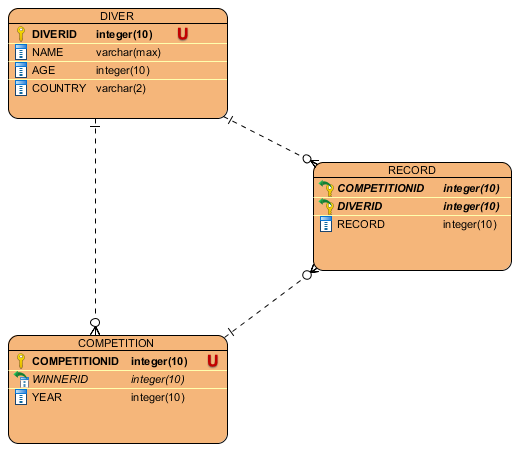
\includegraphics{tablerelation.png}}
\caption{Fig. 1: Entity Relationship Diagram for the DIVER, COMPETITION and RECORD Tables}\end{figure}

DIVER table is the main table for diving section, contains sporters.
COMPETITION table refers to DIVER table, contains diving competitions.
RECORD table refers to both DIVER and COMPETITION tables, contains sporter records.


\paragraph{DIVER:}
\label{developer/member5:diver}
\begin{Verbatim}[commandchars=\\\{\}]
\PYG{k}{CREATE} \PYG{k}{TABLE} \PYG{k}{IF} \PYG{k}{NOT} \PYG{k}{EXISTS} \PYG{n}{DIVER} \PYG{p}{(}
     \PYG{n}{DIVERID} \PYG{n+nb}{INTEGER} \PYG{k}{PRIMARY} \PYG{k}{KEY} \PYG{k}{NOT} \PYG{k}{NULL}\PYG{p}{,}
     \PYG{k}{NAME} \PYG{n+nb}{text}\PYG{p}{,}
     \PYG{n}{AGE} \PYG{n+nb}{INTEGER}\PYG{p}{,}
     \PYG{n}{COUNTRY} \PYG{n+nb}{text}\PYG{p}{)}
\end{Verbatim}

DIVER table contains information about diving sporters.It has 1 major column which is primary key and 3 other information columns.
DIVER table is independent from other tables, it references no other table.

DIVERID is the unique ID of the sporter.
NAME is the name of the sporter.
AGE is the age of the sporter.
COUNTRY is the country which sporter represents.


\paragraph{COMPETITION:}
\label{developer/member5:competition}
\begin{Verbatim}[commandchars=\\\{\}]
\PYG{k}{CREATE} \PYG{k}{TABLE} \PYG{k}{IF} \PYG{k}{NOT} \PYG{k}{EXISTS} \PYG{n}{COMPETITION} \PYG{p}{(}
     \PYG{n}{COMPETITIONID} \PYG{n+nb}{INTEGER} \PYG{k}{PRIMARY} \PYG{k}{KEY} \PYG{k}{NOT} \PYG{k}{NULL}\PYG{p}{,}
     \PYG{n}{WinnerID} \PYG{n+nb}{INTEGER} \PYG{k}{REFERENCES} \PYG{n}{DIVER}\PYG{p}{(}\PYG{n}{DIVERID}\PYG{p}{)} \PYG{k}{ON} \PYG{k}{DELETE} \PYG{k}{RESTRICT} \PYG{k}{ON} \PYG{k}{UPDATE} \PYG{k}{CASCADE}\PYG{p}{,}
     \PYG{k}{YEAR} \PYG{n+nb}{INTEGER}\PYG{p}{)}
\end{Verbatim}

COMPETITION table contains information about diving competitions.
References to DIVER table due to its foreign key WinnerID.

COMPETITIONID is the unique ID of a diving competition.
WINNERID is the ID of the sporter who won the competition.
YEAR is the date which the competition held.


\paragraph{RECORD:}
\label{developer/member5:record}
\begin{Verbatim}[commandchars=\\\{\}]
\PYG{k}{CREATE} \PYG{k}{TABLE} \PYG{k}{IF} \PYG{k}{NOT} \PYG{k}{EXISTS} \PYG{n+nb}{RECORD} \PYG{p}{(}
      \PYG{n}{COMPETITIONID} \PYG{n+nb}{INTEGER} \PYG{k}{REFERENCES} \PYG{n}{COMPETITION}\PYG{p}{(}\PYG{n}{COMPETITIONID}\PYG{p}{)} \PYG{k}{ON} \PYG{k}{DELETE} \PYG{k}{RESTRICT} \PYG{k}{ON} \PYG{k}{UPDATE} \PYG{k}{CASCADE}\PYG{p}{,}
      \PYG{n}{DIVERID} \PYG{n+nb}{INTEGER} \PYG{k}{REFERENCES} \PYG{n}{DIVER}\PYG{p}{(}\PYG{n}{DIVERID}\PYG{p}{)} \PYG{k}{ON} \PYG{k}{DELETE} \PYG{k}{RESTRICT} \PYG{k}{ON} \PYG{k}{UPDATE} \PYG{k}{CASCADE}\PYG{p}{,}
      \PYG{n+nb}{RECORD} \PYG{n+nb}{INTEGER} \PYG{k}{DEFAULT} \PYG{k}{NULL}\PYG{p}{,}
      \PYG{k}{PRIMARY} \PYG{k}{KEY}\PYG{p}{(}\PYG{n}{COMPETITIONID}\PYG{p}{,} \PYG{n}{DIVERID}\PYG{p}{)}\PYG{p}{)}
\end{Verbatim}

RECORD table contains information about sporters record at a specific competition.
It refers to both DIVER table and COMPETITION table via its foreign keys.
Primary key is the combination of COMPETITIONID and DIVERID.

CompetitionID is the unique ID of the competition.
DiverID is the unique ID of the sporter.
Record is the amount of height sporter dived from.


\paragraph{Class codes of Tables from diving.py:}
\label{developer/member5:class-codes-of-tables-from-diving-py}
\begin{Verbatim}[commandchars=\\\{\}]
\PYG{k}{class} \PYG{n+nc}{Diver}\PYG{p}{:}
 \PYG{k}{def} \PYG{n+nf}{\PYGZus{}\PYGZus{}init\PYGZus{}\PYGZus{}}\PYG{p}{(}\PYG{n+nb+bp}{self}\PYG{p}{,} \PYG{n}{diverID}\PYG{p}{,} \PYG{n}{name}\PYG{p}{,} \PYG{n}{age}\PYG{p}{,} \PYG{n}{country}\PYG{p}{)}\PYG{p}{:}
     \PYG{n+nb+bp}{self}\PYG{o}{.}\PYG{n}{diverID} \PYG{o}{=} \PYG{n}{diverID}
     \PYG{n+nb+bp}{self}\PYG{o}{.}\PYG{n}{name} \PYG{o}{=} \PYG{n}{name}
     \PYG{n+nb+bp}{self}\PYG{o}{.}\PYG{n}{age} \PYG{o}{=} \PYG{n}{age}
     \PYG{n+nb+bp}{self}\PYG{o}{.}\PYG{n}{country} \PYG{o}{=} \PYG{n}{country}


\PYG{k}{class} \PYG{n+nc}{Competition}\PYG{p}{:}
 \PYG{k}{def} \PYG{n+nf}{\PYGZus{}\PYGZus{}init\PYGZus{}\PYGZus{}}\PYG{p}{(}\PYG{n+nb+bp}{self}\PYG{p}{,} \PYG{n}{competitionID}\PYG{p}{,} \PYG{n}{winnerID}\PYG{p}{,} \PYG{n}{year}\PYG{p}{)}\PYG{p}{:}
     \PYG{n+nb+bp}{self}\PYG{o}{.}\PYG{n}{competitionID} \PYG{o}{=} \PYG{n}{competitionID}
     \PYG{n+nb+bp}{self}\PYG{o}{.}\PYG{n}{winnerID} \PYG{o}{=} \PYG{n}{winnerID}
     \PYG{n+nb+bp}{self}\PYG{o}{.}\PYG{n}{year} \PYG{o}{=} \PYG{n}{year}

\PYG{k}{class} \PYG{n+nc}{Record}\PYG{p}{:}
 \PYG{k}{def} \PYG{n+nf}{\PYGZus{}\PYGZus{}init\PYGZus{}\PYGZus{}}\PYG{p}{(}\PYG{n+nb+bp}{self}\PYG{p}{,} \PYG{n}{competitionID}\PYG{p}{,} \PYG{n}{diverID}\PYG{p}{,} \PYG{n}{record}\PYG{p}{)}\PYG{p}{:}
     \PYG{n+nb+bp}{self}\PYG{o}{.}\PYG{n}{competitionID} \PYG{o}{=} \PYG{n}{competitionID}
     \PYG{n+nb+bp}{self}\PYG{o}{.}\PYG{n}{diverID} \PYG{o}{=} \PYG{n}{diverID}
     \PYG{n+nb+bp}{self}\PYG{o}{.}\PYG{n}{record} \PYG{o}{=} \PYG{n}{record}
\end{Verbatim}


\paragraph{Diving category codes from server.py file:}
\label{developer/member5:diving-category-codes-from-server-py-file}
add1, update1, delete1 and find1 refers to DIVER table.
add2, update2, delete2 and find2 refers to COMPETITION table.
add3, update3, delete3 and find3 refers to RECORD table.

\begin{Verbatim}[commandchars=\\\{\}]
\PYG{n+nd}{@app.route}\PYG{p}{(}\PYG{l+s}{\PYGZsq{}}\PYG{l+s}{/diving}\PYG{l+s}{\PYGZsq{}}\PYG{p}{,} \PYG{n}{methods}\PYG{o}{=}\PYG{p}{[}\PYG{l+s}{\PYGZsq{}}\PYG{l+s}{GET}\PYG{l+s}{\PYGZsq{}}\PYG{p}{,} \PYG{l+s}{\PYGZsq{}}\PYG{l+s}{POST}\PYG{l+s}{\PYGZsq{}}\PYG{p}{]}\PYG{p}{)}
\PYG{k}{def} \PYG{n+nf}{diving}\PYG{p}{(}\PYG{p}{)}\PYG{p}{:}
 \PYG{n}{ds} \PYG{o}{=} \PYG{n}{DiverStore}\PYG{p}{(}\PYG{n}{app}\PYG{o}{.}\PYG{n}{config}\PYG{p}{[}\PYG{l+s}{\PYGZsq{}}\PYG{l+s}{dsn}\PYG{l+s}{\PYGZsq{}}\PYG{p}{]}\PYG{p}{)}

 \PYG{k}{if} \PYG{n}{request}\PYG{o}{.}\PYG{n}{method} \PYG{o}{==} \PYG{l+s}{\PYGZsq{}}\PYG{l+s}{GET}\PYG{l+s}{\PYGZsq{}}\PYG{p}{:}
     \PYG{k}{return} \PYG{n}{ds}\PYG{o}{.}\PYG{n}{firstrun}\PYG{p}{(}\PYG{p}{)}
 \PYG{k}{else}\PYG{p}{:}
     \PYG{k}{if} \PYG{l+s}{\PYGZsq{}}\PYG{l+s}{add1}\PYG{l+s}{\PYGZsq{}} \PYG{o+ow}{in} \PYG{n}{request}\PYG{o}{.}\PYG{n}{form}\PYG{p}{:}
         \PYG{n}{diverID} \PYG{o}{=} \PYG{n}{request}\PYG{o}{.}\PYG{n}{form}\PYG{p}{[}\PYG{l+s}{\PYGZsq{}}\PYG{l+s}{id}\PYG{l+s}{\PYGZsq{}}\PYG{p}{]}
         \PYG{n}{name} \PYG{o}{=} \PYG{n}{request}\PYG{o}{.}\PYG{n}{form}\PYG{p}{[}\PYG{l+s}{\PYGZsq{}}\PYG{l+s}{name}\PYG{l+s}{\PYGZsq{}}\PYG{p}{]}
         \PYG{n}{age} \PYG{o}{=} \PYG{n}{request}\PYG{o}{.}\PYG{n}{form}\PYG{p}{[}\PYG{l+s}{\PYGZsq{}}\PYG{l+s}{age}\PYG{l+s}{\PYGZsq{}}\PYG{p}{]}
         \PYG{n}{country} \PYG{o}{=} \PYG{n}{request}\PYG{o}{.}\PYG{n}{form}\PYG{p}{[}\PYG{l+s}{\PYGZsq{}}\PYG{l+s}{country}\PYG{l+s}{\PYGZsq{}}\PYG{p}{]}
         \PYG{k}{return} \PYG{n}{ds}\PYG{o}{.}\PYG{n}{add\PYGZus{}diver}\PYG{p}{(}\PYG{n}{Diver}\PYG{p}{(}\PYG{n}{diverID}\PYG{p}{,} \PYG{n}{name}\PYG{p}{,} \PYG{n}{age}\PYG{p}{,} \PYG{n}{country}\PYG{p}{)}\PYG{p}{,} \PYG{l+m+mi}{1}\PYG{p}{)}
     \PYG{k}{elif} \PYG{l+s}{\PYGZsq{}}\PYG{l+s}{add2}\PYG{l+s}{\PYGZsq{}} \PYG{o+ow}{in} \PYG{n}{request}\PYG{o}{.}\PYG{n}{form}\PYG{p}{:}
         \PYG{n}{competitionID} \PYG{o}{=} \PYG{n}{request}\PYG{o}{.}\PYG{n}{form}\PYG{p}{[}\PYG{l+s}{\PYGZsq{}}\PYG{l+s}{competitionID}\PYG{l+s}{\PYGZsq{}}\PYG{p}{]}
         \PYG{n}{winnerID} \PYG{o}{=} \PYG{n}{request}\PYG{o}{.}\PYG{n}{form}\PYG{p}{[}\PYG{l+s}{\PYGZsq{}}\PYG{l+s}{winnerID}\PYG{l+s}{\PYGZsq{}}\PYG{p}{]}
         \PYG{n}{year} \PYG{o}{=} \PYG{n}{request}\PYG{o}{.}\PYG{n}{form}\PYG{p}{[}\PYG{l+s}{\PYGZsq{}}\PYG{l+s}{year}\PYG{l+s}{\PYGZsq{}}\PYG{p}{]}
         \PYG{k}{return} \PYG{n}{ds}\PYG{o}{.}\PYG{n}{add\PYGZus{}diver}\PYG{p}{(}\PYG{n}{Competition}\PYG{p}{(}\PYG{n}{competitionID}\PYG{p}{,} \PYG{n}{winnerID}\PYG{p}{,} \PYG{n}{year}\PYG{p}{)}\PYG{p}{,} \PYG{l+m+mi}{2}\PYG{p}{)}
     \PYG{k}{elif} \PYG{l+s}{\PYGZsq{}}\PYG{l+s}{add3}\PYG{l+s}{\PYGZsq{}} \PYG{o+ow}{in} \PYG{n}{request}\PYG{o}{.}\PYG{n}{form}\PYG{p}{:}
         \PYG{n}{competitionID} \PYG{o}{=} \PYG{n}{request}\PYG{o}{.}\PYG{n}{form}\PYG{p}{[}\PYG{l+s}{\PYGZsq{}}\PYG{l+s}{competitionID}\PYG{l+s}{\PYGZsq{}}\PYG{p}{]}
         \PYG{n}{diverID} \PYG{o}{=} \PYG{n}{request}\PYG{o}{.}\PYG{n}{form}\PYG{p}{[}\PYG{l+s}{\PYGZsq{}}\PYG{l+s}{diverID}\PYG{l+s}{\PYGZsq{}}\PYG{p}{]}
         \PYG{n}{record} \PYG{o}{=} \PYG{n}{request}\PYG{o}{.}\PYG{n}{form}\PYG{p}{[}\PYG{l+s}{\PYGZsq{}}\PYG{l+s}{record}\PYG{l+s}{\PYGZsq{}}\PYG{p}{]}
         \PYG{k}{return} \PYG{n}{ds}\PYG{o}{.}\PYG{n}{add\PYGZus{}diver}\PYG{p}{(}\PYG{n}{Record}\PYG{p}{(}\PYG{n}{competitionID}\PYG{p}{,} \PYG{n}{diverID}\PYG{p}{,} \PYG{n}{record}\PYG{p}{)}\PYG{p}{,} \PYG{l+m+mi}{3}\PYG{p}{)}


     \PYG{k}{elif} \PYG{l+s}{\PYGZsq{}}\PYG{l+s}{update1}\PYG{l+s}{\PYGZsq{}} \PYG{o+ow}{in} \PYG{n}{request}\PYG{o}{.}\PYG{n}{form}\PYG{p}{:}
         \PYG{n}{diverID} \PYG{o}{=} \PYG{n}{request}\PYG{o}{.}\PYG{n}{form}\PYG{p}{[}\PYG{l+s}{\PYGZsq{}}\PYG{l+s}{id}\PYG{l+s}{\PYGZsq{}}\PYG{p}{]}
         \PYG{n}{name} \PYG{o}{=} \PYG{n}{request}\PYG{o}{.}\PYG{n}{form}\PYG{p}{[}\PYG{l+s}{\PYGZsq{}}\PYG{l+s}{name}\PYG{l+s}{\PYGZsq{}}\PYG{p}{]}
         \PYG{n}{age} \PYG{o}{=} \PYG{n}{request}\PYG{o}{.}\PYG{n}{form}\PYG{p}{[}\PYG{l+s}{\PYGZsq{}}\PYG{l+s}{age}\PYG{l+s}{\PYGZsq{}}\PYG{p}{]}
         \PYG{n}{country} \PYG{o}{=} \PYG{n}{request}\PYG{o}{.}\PYG{n}{form}\PYG{p}{[}\PYG{l+s}{\PYGZsq{}}\PYG{l+s}{country}\PYG{l+s}{\PYGZsq{}}\PYG{p}{]}
         \PYG{n}{searchID} \PYG{o}{=} \PYG{n}{request}\PYG{o}{.}\PYG{n}{form}\PYG{p}{[}\PYG{l+s}{\PYGZsq{}}\PYG{l+s}{select}\PYG{l+s}{\PYGZsq{}}\PYG{p}{]}
         \PYG{k}{return} \PYG{n}{ds}\PYG{o}{.}\PYG{n}{update\PYGZus{}diver}\PYG{p}{(}\PYG{n}{Diver}\PYG{p}{(}\PYG{n}{diverID}\PYG{p}{,} \PYG{n}{name}\PYG{p}{,} \PYG{n}{age}\PYG{p}{,} \PYG{n}{country}\PYG{p}{)}\PYG{p}{,} \PYG{n}{searchID}\PYG{p}{,} \PYG{l+m+mi}{1}\PYG{p}{)}
     \PYG{k}{elif} \PYG{l+s}{\PYGZsq{}}\PYG{l+s}{update2}\PYG{l+s}{\PYGZsq{}} \PYG{o+ow}{in} \PYG{n}{request}\PYG{o}{.}\PYG{n}{form}\PYG{p}{:}
         \PYG{n}{competitionID} \PYG{o}{=} \PYG{n}{request}\PYG{o}{.}\PYG{n}{form}\PYG{p}{[}\PYG{l+s}{\PYGZsq{}}\PYG{l+s}{competitionID}\PYG{l+s}{\PYGZsq{}}\PYG{p}{]}
         \PYG{n}{winnerID} \PYG{o}{=} \PYG{n}{request}\PYG{o}{.}\PYG{n}{form}\PYG{p}{[}\PYG{l+s}{\PYGZsq{}}\PYG{l+s}{winnerID}\PYG{l+s}{\PYGZsq{}}\PYG{p}{]}
         \PYG{n}{year} \PYG{o}{=} \PYG{n}{request}\PYG{o}{.}\PYG{n}{form}\PYG{p}{[}\PYG{l+s}{\PYGZsq{}}\PYG{l+s}{year}\PYG{l+s}{\PYGZsq{}}\PYG{p}{]}
         \PYG{n}{searchID} \PYG{o}{=} \PYG{n}{request}\PYG{o}{.}\PYG{n}{form}\PYG{p}{[}\PYG{l+s}{\PYGZsq{}}\PYG{l+s}{select}\PYG{l+s}{\PYGZsq{}}\PYG{p}{]}
         \PYG{k}{return} \PYG{n}{ds}\PYG{o}{.}\PYG{n}{update\PYGZus{}diver}\PYG{p}{(}\PYG{n}{Competition}\PYG{p}{(}\PYG{n}{competitionID}\PYG{p}{,} \PYG{n}{winnerID}\PYG{p}{,} \PYG{n}{year}\PYG{p}{)}\PYG{p}{,} \PYG{n}{searchID}\PYG{p}{,} \PYG{l+m+mi}{2}\PYG{p}{)}
     \PYG{k}{elif} \PYG{l+s}{\PYGZsq{}}\PYG{l+s}{update3}\PYG{l+s}{\PYGZsq{}} \PYG{o+ow}{in} \PYG{n}{request}\PYG{o}{.}\PYG{n}{form}\PYG{p}{:}
         \PYG{n}{competitionID} \PYG{o}{=} \PYG{n}{request}\PYG{o}{.}\PYG{n}{form}\PYG{p}{[}\PYG{l+s}{\PYGZsq{}}\PYG{l+s}{competitionID}\PYG{l+s}{\PYGZsq{}}\PYG{p}{]}
         \PYG{n}{diverID} \PYG{o}{=} \PYG{n}{request}\PYG{o}{.}\PYG{n}{form}\PYG{p}{[}\PYG{l+s}{\PYGZsq{}}\PYG{l+s}{diverID}\PYG{l+s}{\PYGZsq{}}\PYG{p}{]}
         \PYG{n}{record} \PYG{o}{=} \PYG{n}{request}\PYG{o}{.}\PYG{n}{form}\PYG{p}{[}\PYG{l+s}{\PYGZsq{}}\PYG{l+s}{record}\PYG{l+s}{\PYGZsq{}}\PYG{p}{]}
         \PYG{n}{combinedSearchID} \PYG{o}{=} \PYG{n}{request}\PYG{o}{.}\PYG{n}{form}\PYG{p}{[}\PYG{l+s}{\PYGZsq{}}\PYG{l+s}{select}\PYG{l+s}{\PYGZsq{}}\PYG{p}{]}
         \PYG{k}{return} \PYG{n}{ds}\PYG{o}{.}\PYG{n}{update\PYGZus{}diver}\PYG{p}{(}\PYG{n}{Record}\PYG{p}{(}\PYG{n}{competitionID}\PYG{p}{,} \PYG{n}{diverID}\PYG{p}{,} \PYG{n}{record}\PYG{p}{)}\PYG{p}{,} \PYG{n}{combinedSearchID}\PYG{p}{,} \PYG{l+m+mi}{3}\PYG{p}{)}


     \PYG{k}{elif} \PYG{l+s}{\PYGZsq{}}\PYG{l+s}{find1}\PYG{l+s}{\PYGZsq{}} \PYG{o+ow}{in} \PYG{n}{request}\PYG{o}{.}\PYG{n}{form}\PYG{p}{:}
         \PYG{n}{diverID} \PYG{o}{=} \PYG{n}{request}\PYG{o}{.}\PYG{n}{form}\PYG{p}{[}\PYG{l+s}{\PYGZsq{}}\PYG{l+s}{id}\PYG{l+s}{\PYGZsq{}}\PYG{p}{]}
         \PYG{n}{name} \PYG{o}{=} \PYG{n}{request}\PYG{o}{.}\PYG{n}{form}\PYG{p}{[}\PYG{l+s}{\PYGZsq{}}\PYG{l+s}{name}\PYG{l+s}{\PYGZsq{}}\PYG{p}{]}
         \PYG{n}{age} \PYG{o}{=} \PYG{n}{request}\PYG{o}{.}\PYG{n}{form}\PYG{p}{[}\PYG{l+s}{\PYGZsq{}}\PYG{l+s}{age}\PYG{l+s}{\PYGZsq{}}\PYG{p}{]}
         \PYG{n}{country} \PYG{o}{=} \PYG{n}{request}\PYG{o}{.}\PYG{n}{form}\PYG{p}{[}\PYG{l+s}{\PYGZsq{}}\PYG{l+s}{country}\PYG{l+s}{\PYGZsq{}}\PYG{p}{]}
         \PYG{k}{return} \PYG{n}{ds}\PYG{o}{.}\PYG{n}{find\PYGZus{}diver}\PYG{p}{(}\PYG{n}{Diver}\PYG{p}{(}\PYG{n}{diverID}\PYG{p}{,} \PYG{n}{name}\PYG{p}{,} \PYG{n}{age}\PYG{p}{,} \PYG{n}{country}\PYG{p}{)}\PYG{p}{,} \PYG{l+m+mi}{1}\PYG{p}{)}
     \PYG{k}{elif} \PYG{l+s}{\PYGZsq{}}\PYG{l+s}{find2}\PYG{l+s}{\PYGZsq{}} \PYG{o+ow}{in} \PYG{n}{request}\PYG{o}{.}\PYG{n}{form}\PYG{p}{:}
         \PYG{n}{competitionID} \PYG{o}{=} \PYG{n}{request}\PYG{o}{.}\PYG{n}{form}\PYG{p}{[}\PYG{l+s}{\PYGZsq{}}\PYG{l+s}{competitionID}\PYG{l+s}{\PYGZsq{}}\PYG{p}{]}
         \PYG{n}{winnerID} \PYG{o}{=} \PYG{n}{request}\PYG{o}{.}\PYG{n}{form}\PYG{p}{[}\PYG{l+s}{\PYGZsq{}}\PYG{l+s}{winnerID}\PYG{l+s}{\PYGZsq{}}\PYG{p}{]}
         \PYG{n}{year} \PYG{o}{=} \PYG{n}{request}\PYG{o}{.}\PYG{n}{form}\PYG{p}{[}\PYG{l+s}{\PYGZsq{}}\PYG{l+s}{year}\PYG{l+s}{\PYGZsq{}}\PYG{p}{]}
         \PYG{k}{return} \PYG{n}{ds}\PYG{o}{.}\PYG{n}{find\PYGZus{}diver}\PYG{p}{(}\PYG{n}{Competition}\PYG{p}{(}\PYG{n}{competitionID}\PYG{p}{,} \PYG{n}{winnerID}\PYG{p}{,} \PYG{n}{year}\PYG{p}{)}\PYG{p}{,} \PYG{l+m+mi}{2}\PYG{p}{)}
     \PYG{k}{elif} \PYG{l+s}{\PYGZsq{}}\PYG{l+s}{find3}\PYG{l+s}{\PYGZsq{}} \PYG{o+ow}{in} \PYG{n}{request}\PYG{o}{.}\PYG{n}{form}\PYG{p}{:}
         \PYG{n}{competitionID} \PYG{o}{=} \PYG{n}{request}\PYG{o}{.}\PYG{n}{form}\PYG{p}{[}\PYG{l+s}{\PYGZsq{}}\PYG{l+s}{competitionID}\PYG{l+s}{\PYGZsq{}}\PYG{p}{]}
         \PYG{n}{diverID} \PYG{o}{=} \PYG{n}{request}\PYG{o}{.}\PYG{n}{form}\PYG{p}{[}\PYG{l+s}{\PYGZsq{}}\PYG{l+s}{diverID}\PYG{l+s}{\PYGZsq{}}\PYG{p}{]}
         \PYG{n}{record} \PYG{o}{=} \PYG{n}{request}\PYG{o}{.}\PYG{n}{form}\PYG{p}{[}\PYG{l+s}{\PYGZsq{}}\PYG{l+s}{record}\PYG{l+s}{\PYGZsq{}}\PYG{p}{]}
         \PYG{k}{return} \PYG{n}{ds}\PYG{o}{.}\PYG{n}{find\PYGZus{}diver}\PYG{p}{(}\PYG{n}{Record}\PYG{p}{(}\PYG{n}{competitionID}\PYG{p}{,} \PYG{n}{diverID}\PYG{p}{,} \PYG{n}{record}\PYG{p}{)}\PYG{p}{,} \PYG{l+m+mi}{3}\PYG{p}{)}


     \PYG{k}{elif} \PYG{l+s}{\PYGZsq{}}\PYG{l+s}{recreate}\PYG{l+s}{\PYGZsq{}} \PYG{o+ow}{in} \PYG{n}{request}\PYG{o}{.}\PYG{n}{form}\PYG{p}{:}
         \PYG{c}{\PYGZsh{}  create new tables and add some rows}
         \PYG{n}{ds}\PYG{o}{.}\PYG{n}{recreate}\PYG{p}{(}\PYG{p}{)}
         \PYG{k}{return} \PYG{n}{redirect}\PYG{p}{(}\PYG{n}{url\PYGZus{}for}\PYG{p}{(}\PYG{l+s}{\PYGZsq{}}\PYG{l+s}{diving}\PYG{l+s}{\PYGZsq{}}\PYG{p}{)}\PYG{p}{)}
     \PYG{k}{elif} \PYG{l+s}{\PYGZsq{}}\PYG{l+s}{return}\PYG{l+s}{\PYGZsq{}} \PYG{o+ow}{in} \PYG{n}{request}\PYG{o}{.}\PYG{n}{form}\PYG{p}{:}
         \PYG{c}{\PYGZsh{}  return to main diving page}
          \PYG{k}{return} \PYG{n}{redirect}\PYG{p}{(}\PYG{n}{url\PYGZus{}for}\PYG{p}{(}\PYG{l+s}{\PYGZsq{}}\PYG{l+s}{diving}\PYG{l+s}{\PYGZsq{}}\PYG{p}{)}\PYG{p}{)}
\end{Verbatim}


\paragraph{Add operation from diving.py file:}
\label{developer/member5:add-operation-from-diving-py-file}
\begin{Verbatim}[commandchars=\\\{\}]
\PYG{k}{def} \PYG{n+nf}{add\PYGZus{}diver}\PYG{p}{(}\PYG{n+nb+bp}{self}\PYG{p}{,} \PYG{n}{data}\PYG{p}{,} \PYG{n}{table}\PYG{p}{)}\PYG{p}{:}
     \PYG{k}{try}\PYG{p}{:}
         \PYG{n}{ValidateInput}\PYG{p}{(}\PYG{n}{data}\PYG{p}{,} \PYG{n}{table}\PYG{p}{)}
     \PYG{k}{except} \PYG{n+ne}{ValueError}\PYG{p}{:}
         \PYG{k}{return} \PYG{n}{render\PYGZus{}template}\PYG{p}{(}\PYG{l+s}{\PYGZsq{}}\PYG{l+s}{Diving/InvalidValue.html}\PYG{l+s}{\PYGZsq{}}\PYG{p}{,} \PYG{n}{divers}\PYG{o}{=}\PYG{n}{divers}\PYG{p}{)}

     \PYG{k}{with} \PYG{n}{dbapi2}\PYG{o}{.}\PYG{n}{connect}\PYG{p}{(}\PYG{n+nb+bp}{self}\PYG{o}{.}\PYG{n}{dbf}\PYG{p}{)} \PYG{k}{as} \PYG{n}{connection}\PYG{p}{:}
         \PYG{n}{cursor} \PYG{o}{=} \PYG{n}{connection}\PYG{o}{.}\PYG{n}{cursor}\PYG{p}{(}\PYG{p}{)}
         \PYG{n}{query} \PYG{o}{=} \PYG{l+s}{\PYGZdq{}}\PYG{l+s}{\PYGZdq{}}

         \PYG{k}{if} \PYG{n}{table} \PYG{o}{==} \PYG{l+m+mi}{1}\PYG{p}{:}
             \PYG{n}{query} \PYG{o}{=} \PYG{l+s}{\PYGZdq{}\PYGZdq{}\PYGZdq{}}\PYG{l+s}{INSERT INTO DIVER (DIVERID, NAME, AGE, COUNTRY)}
\PYG{l+s}{                         VALUES (}\PYG{l+s}{\PYGZsq{}}\PYG{l+s+si}{\PYGZpc{}s}\PYG{l+s}{\PYGZsq{}}\PYG{l+s}{, }\PYG{l+s}{\PYGZsq{}}\PYG{l+s+si}{\PYGZpc{}s}\PYG{l+s}{\PYGZsq{}}\PYG{l+s}{, }\PYG{l+s}{\PYGZsq{}}\PYG{l+s+si}{\PYGZpc{}s}\PYG{l+s}{\PYGZsq{}}\PYG{l+s}{, }\PYG{l+s}{\PYGZsq{}}\PYG{l+s+si}{\PYGZpc{}s}\PYG{l+s}{\PYGZsq{}}\PYG{l+s}{)}\PYG{l+s}{\PYGZdq{}\PYGZdq{}\PYGZdq{}} \PYG{o}{\PYGZpc{}} \PYG{p}{(}\PYG{n}{data}\PYG{o}{.}\PYG{n}{diverID}\PYG{p}{,} \PYG{n}{data}\PYG{o}{.}\PYG{n}{name}\PYG{p}{,} \PYG{n}{data}\PYG{o}{.}\PYG{n}{age}\PYG{p}{,} \PYG{n}{data}\PYG{o}{.}\PYG{n}{country}\PYG{p}{)}
         \PYG{k}{elif} \PYG{n}{table} \PYG{o}{==} \PYG{l+m+mi}{2}\PYG{p}{:}
             \PYG{n}{query} \PYG{o}{=} \PYG{l+s}{\PYGZdq{}\PYGZdq{}\PYGZdq{}}\PYG{l+s}{INSERT INTO COMPETITION (COMPETITIONID, WinnerID, YEAR)}
\PYG{l+s}{                         VALUES (}\PYG{l+s}{\PYGZsq{}}\PYG{l+s+si}{\PYGZpc{}s}\PYG{l+s}{\PYGZsq{}}\PYG{l+s}{, }\PYG{l+s}{\PYGZsq{}}\PYG{l+s+si}{\PYGZpc{}s}\PYG{l+s}{\PYGZsq{}}\PYG{l+s}{, }\PYG{l+s}{\PYGZsq{}}\PYG{l+s+si}{\PYGZpc{}s}\PYG{l+s}{\PYGZsq{}}\PYG{l+s}{)}\PYG{l+s}{\PYGZdq{}\PYGZdq{}\PYGZdq{}} \PYG{o}{\PYGZpc{}} \PYG{p}{(}\PYG{n}{data}\PYG{o}{.}\PYG{n}{competitionID}\PYG{p}{,} \PYG{n}{data}\PYG{o}{.}\PYG{n}{winnerID}\PYG{p}{,} \PYG{n}{data}\PYG{o}{.}\PYG{n}{year}\PYG{p}{)}
         \PYG{k}{elif} \PYG{n}{table} \PYG{o}{==} \PYG{l+m+mi}{3}\PYG{p}{:}
             \PYG{n}{query} \PYG{o}{=} \PYG{l+s}{\PYGZdq{}\PYGZdq{}\PYGZdq{}}\PYG{l+s}{INSERT INTO RECORD (COMPETITIONID, DIVERID, Record)}
\PYG{l+s}{                         VALUES (}\PYG{l+s}{\PYGZsq{}}\PYG{l+s+si}{\PYGZpc{}s}\PYG{l+s}{\PYGZsq{}}\PYG{l+s}{, }\PYG{l+s}{\PYGZsq{}}\PYG{l+s+si}{\PYGZpc{}s}\PYG{l+s}{\PYGZsq{}}\PYG{l+s}{, }\PYG{l+s}{\PYGZsq{}}\PYG{l+s+si}{\PYGZpc{}s}\PYG{l+s}{\PYGZsq{}}\PYG{l+s}{)}\PYG{l+s}{\PYGZdq{}\PYGZdq{}\PYGZdq{}} \PYG{o}{\PYGZpc{}} \PYG{p}{(}\PYG{n}{data}\PYG{o}{.}\PYG{n}{competitionID}\PYG{p}{,} \PYG{n}{data}\PYG{o}{.}\PYG{n}{diverID}\PYG{p}{,} \PYG{n}{data}\PYG{o}{.}\PYG{n}{record}\PYG{p}{)}

         \PYG{n}{cursor}\PYG{o}{.}\PYG{n}{execute}\PYG{p}{(}\PYG{n}{query}\PYG{p}{)}
         \PYG{n}{connection}\PYG{o}{.}\PYG{n}{commit}\PYG{p}{(}\PYG{p}{)}
         \PYG{k}{return} \PYG{n}{redirect}\PYG{p}{(}\PYG{n}{url\PYGZus{}for}\PYG{p}{(}\PYG{l+s}{\PYGZsq{}}\PYG{l+s}{diving}\PYG{l+s}{\PYGZsq{}}\PYG{p}{)}\PYG{p}{)}
\end{Verbatim}


\paragraph{Update operation from diving.py file:}
\label{developer/member5:update-operation-from-diving-py-file}
\begin{Verbatim}[commandchars=\\\{\}]
\PYG{k}{def} \PYG{n+nf}{update\PYGZus{}diver}\PYG{p}{(}\PYG{n+nb+bp}{self}\PYG{p}{,} \PYG{n}{data}\PYG{p}{,} \PYG{n+nb}{id}\PYG{p}{,} \PYG{n}{table}\PYG{p}{)}\PYG{p}{:}
     \PYG{k}{try}\PYG{p}{:}
         \PYG{n}{ValidateInput}\PYG{p}{(}\PYG{n}{data}\PYG{p}{,} \PYG{n}{table}\PYG{p}{)}
     \PYG{k}{except} \PYG{n+ne}{ValueError}\PYG{p}{:}
         \PYG{k}{return} \PYG{n}{render\PYGZus{}template}\PYG{p}{(}\PYG{l+s}{\PYGZsq{}}\PYG{l+s}{Diving/InvalidValue.html}\PYG{l+s}{\PYGZsq{}}\PYG{p}{,} \PYG{n}{divers}\PYG{o}{=}\PYG{n}{divers}\PYG{p}{)}

     \PYG{k}{with} \PYG{n}{dbapi2}\PYG{o}{.}\PYG{n}{connect}\PYG{p}{(}\PYG{n+nb+bp}{self}\PYG{o}{.}\PYG{n}{dbf}\PYG{p}{)} \PYG{k}{as} \PYG{n}{connection}\PYG{p}{:}
         \PYG{n}{cursor} \PYG{o}{=} \PYG{n}{connection}\PYG{o}{.}\PYG{n}{cursor}\PYG{p}{(}\PYG{p}{)}
         \PYG{n}{query} \PYG{o}{=} \PYG{l+s}{\PYGZdq{}}\PYG{l+s}{\PYGZdq{}}

         \PYG{k}{if} \PYG{n}{table} \PYG{o}{==} \PYG{l+m+mi}{1}\PYG{p}{:}
             \PYG{n}{query} \PYG{o}{=} \PYG{l+s}{\PYGZdq{}\PYGZdq{}\PYGZdq{}}\PYG{l+s}{UPDATE DIVER}
\PYG{l+s}{                         SET DIVERID=}\PYG{l+s}{\PYGZsq{}}\PYG{l+s+si}{\PYGZpc{}s}\PYG{l+s}{\PYGZsq{}}\PYG{l+s}{, NAME=}\PYG{l+s}{\PYGZsq{}}\PYG{l+s+si}{\PYGZpc{}s}\PYG{l+s}{\PYGZsq{}}\PYG{l+s}{, AGE=}\PYG{l+s}{\PYGZsq{}}\PYG{l+s+si}{\PYGZpc{}s}\PYG{l+s}{\PYGZsq{}}\PYG{l+s}{, COUNTRY=}\PYG{l+s}{\PYGZsq{}}\PYG{l+s+si}{\PYGZpc{}s}\PYG{l+s}{\PYGZsq{}}
\PYG{l+s}{                         WHERE (DIVERID = }\PYG{l+s}{\PYGZsq{}}\PYG{l+s+si}{\PYGZpc{}s}\PYG{l+s}{\PYGZsq{}}\PYG{l+s}{)}\PYG{l+s}{\PYGZdq{}\PYGZdq{}\PYGZdq{}} \PYG{o}{\PYGZpc{}} \PYG{p}{(}\PYG{n}{data}\PYG{o}{.}\PYG{n}{diverID}\PYG{p}{,} \PYG{n}{data}\PYG{o}{.}\PYG{n}{name}\PYG{p}{,} \PYG{n}{data}\PYG{o}{.}\PYG{n}{age}\PYG{p}{,} \PYG{n}{data}\PYG{o}{.}\PYG{n}{country}\PYG{p}{,} \PYG{n+nb}{id}\PYG{p}{)}
         \PYG{k}{elif} \PYG{n}{table} \PYG{o}{==} \PYG{l+m+mi}{2}\PYG{p}{:}
             \PYG{n}{query} \PYG{o}{=} \PYG{l+s}{\PYGZdq{}\PYGZdq{}\PYGZdq{}}\PYG{l+s}{UPDATE COMPETITION}
\PYG{l+s}{                         SET COMPETITIONID=}\PYG{l+s}{\PYGZsq{}}\PYG{l+s+si}{\PYGZpc{}s}\PYG{l+s}{\PYGZsq{}}\PYG{l+s}{, WinnerID=}\PYG{l+s}{\PYGZsq{}}\PYG{l+s+si}{\PYGZpc{}s}\PYG{l+s}{\PYGZsq{}}\PYG{l+s}{, YEAR=}\PYG{l+s}{\PYGZsq{}}\PYG{l+s+si}{\PYGZpc{}s}\PYG{l+s}{\PYGZsq{}}
\PYG{l+s}{                         WHERE (COMPETITIONID = }\PYG{l+s}{\PYGZsq{}}\PYG{l+s+si}{\PYGZpc{}s}\PYG{l+s}{\PYGZsq{}}\PYG{l+s}{)}\PYG{l+s}{\PYGZdq{}\PYGZdq{}\PYGZdq{}} \PYG{o}{\PYGZpc{}} \PYG{p}{(}\PYG{n}{data}\PYG{o}{.}\PYG{n}{competitionID}\PYG{p}{,} \PYG{n}{data}\PYG{o}{.}\PYG{n}{winnerID}\PYG{p}{,} \PYG{n}{data}\PYG{o}{.}\PYG{n}{year}\PYG{p}{,} \PYG{n+nb}{id}\PYG{p}{)}
         \PYG{k}{elif} \PYG{n}{table} \PYG{o}{==} \PYG{l+m+mi}{3}\PYG{p}{:}
             \PYG{n}{ids} \PYG{o}{=} \PYG{n+nb}{id}\PYG{o}{.}\PYG{n}{split}\PYG{p}{(}\PYG{l+s}{\PYGZsq{}}\PYG{l+s}{\PYGZhy{}}\PYG{l+s}{\PYGZsq{}}\PYG{p}{)}
             \PYG{n}{query} \PYG{o}{=} \PYG{l+s}{\PYGZdq{}\PYGZdq{}\PYGZdq{}}\PYG{l+s}{UPDATE DIVER}
\PYG{l+s}{                         SET COMPETITIONID=}\PYG{l+s}{\PYGZsq{}}\PYG{l+s+si}{\PYGZpc{}s}\PYG{l+s}{\PYGZsq{}}\PYG{l+s}{, DIVERID=}\PYG{l+s}{\PYGZsq{}}\PYG{l+s+si}{\PYGZpc{}s}\PYG{l+s}{\PYGZsq{}}\PYG{l+s}{, RECORD=}\PYG{l+s}{\PYGZsq{}}\PYG{l+s+si}{\PYGZpc{}s}\PYG{l+s}{\PYGZsq{}}
\PYG{l+s}{                         WHERE ((COMPETITIONID = }\PYG{l+s}{\PYGZsq{}}\PYG{l+s+si}{\PYGZpc{}s}\PYG{l+s}{\PYGZsq{}}\PYG{l+s}{) AND (DIVERID = }\PYG{l+s}{\PYGZsq{}}\PYG{l+s+si}{\PYGZpc{}s}\PYG{l+s}{\PYGZsq{}}\PYG{l+s}{))}\PYG{l+s}{\PYGZdq{}\PYGZdq{}\PYGZdq{}} \PYG{o}{\PYGZpc{}} \PYG{p}{(}\PYG{n}{data}\PYG{o}{.}\PYG{n}{competitionID}\PYG{p}{,} \PYG{n}{data}\PYG{o}{.}\PYG{n}{diverID}\PYG{p}{,} \PYG{n}{data}\PYG{o}{.}\PYG{n}{record}\PYG{p}{,} \PYG{n}{ids}\PYG{p}{[}\PYG{l+m+mi}{0}\PYG{p}{]}\PYG{p}{,} \PYG{n}{ids}\PYG{p}{[}\PYG{l+m+mi}{1}\PYG{p}{]}\PYG{p}{)}

         \PYG{n}{cursor}\PYG{o}{.}\PYG{n}{execute}\PYG{p}{(}\PYG{n}{query}\PYG{p}{)}
         \PYG{n}{connection}\PYG{o}{.}\PYG{n}{commit}\PYG{p}{(}\PYG{p}{)}
         \PYG{k}{return} \PYG{n}{redirect}\PYG{p}{(}\PYG{n}{url\PYGZus{}for}\PYG{p}{(}\PYG{l+s}{\PYGZsq{}}\PYG{l+s}{diving}\PYG{l+s}{\PYGZsq{}}\PYG{p}{)}\PYG{p}{)}
\end{Verbatim}


\paragraph{Delete operation from diving.py file:}
\label{developer/member5:delete-operation-from-diving-py-file}
Deletes a record from database by ID

\begin{Verbatim}[commandchars=\\\{\}]
\PYG{k}{def} \PYG{n+nf}{delete\PYGZus{}diver}\PYG{p}{(}\PYG{n+nb+bp}{self}\PYG{p}{,} \PYG{n+nb}{id}\PYG{p}{,} \PYG{n}{table}\PYG{p}{)}\PYG{p}{:}
     \PYG{k}{with} \PYG{n}{dbapi2}\PYG{o}{.}\PYG{n}{connect}\PYG{p}{(}\PYG{n+nb+bp}{self}\PYG{o}{.}\PYG{n}{dbf}\PYG{p}{)} \PYG{k}{as} \PYG{n}{connection}\PYG{p}{:}
         \PYG{n}{cursor} \PYG{o}{=} \PYG{n}{connection}\PYG{o}{.}\PYG{n}{cursor}\PYG{p}{(}\PYG{p}{)}
         \PYG{n}{query} \PYG{o}{=} \PYG{l+s}{\PYGZdq{}}\PYG{l+s}{\PYGZdq{}}

         \PYG{k}{if} \PYG{n}{table} \PYG{o}{==} \PYG{l+m+mi}{1}\PYG{p}{:}
             \PYG{n}{query} \PYG{o}{=} \PYG{l+s}{\PYGZdq{}}\PYG{l+s}{DELETE FROM DIVER WHERE (DIVERID = }\PYG{l+s}{\PYGZsq{}}\PYG{l+s+si}{\PYGZpc{}s}\PYG{l+s}{\PYGZsq{}}\PYG{l+s}{)}\PYG{l+s}{\PYGZdq{}} \PYG{o}{\PYGZpc{}}\PYG{p}{(}\PYG{n+nb}{id}\PYG{p}{)}
         \PYG{k}{elif} \PYG{n}{table} \PYG{o}{==} \PYG{l+m+mi}{2}\PYG{p}{:}
             \PYG{n}{query} \PYG{o}{=} \PYG{l+s}{\PYGZdq{}}\PYG{l+s}{DELETE FROM COMPETITION WHERE (COMPETITIONID = }\PYG{l+s}{\PYGZsq{}}\PYG{l+s+si}{\PYGZpc{}s}\PYG{l+s}{\PYGZsq{}}\PYG{l+s}{)}\PYG{l+s}{\PYGZdq{}} \PYG{o}{\PYGZpc{}}\PYG{p}{(}\PYG{n+nb}{id}\PYG{p}{)}
         \PYG{k}{elif} \PYG{n}{table} \PYG{o}{==} \PYG{l+m+mi}{3}\PYG{p}{:}
             \PYG{n}{ids} \PYG{o}{=} \PYG{n+nb}{id}\PYG{o}{.}\PYG{n}{split}\PYG{p}{(}\PYG{l+s}{\PYGZsq{}}\PYG{l+s}{\PYGZhy{}}\PYG{l+s}{\PYGZsq{}}\PYG{p}{)}
             \PYG{n}{query} \PYG{o}{=} \PYG{l+s}{\PYGZdq{}}\PYG{l+s}{DELETE FROM RECORD WHERE ((COMPETITIONID = }\PYG{l+s}{\PYGZsq{}}\PYG{l+s+si}{\PYGZpc{}s}\PYG{l+s}{\PYGZsq{}}\PYG{l+s}{) AND (DIVERID = }\PYG{l+s}{\PYGZsq{}}\PYG{l+s+si}{\PYGZpc{}s}\PYG{l+s}{\PYGZsq{}}\PYG{l+s}{))}\PYG{l+s}{\PYGZdq{}} \PYG{o}{\PYGZpc{}}\PYG{p}{(}\PYG{n}{ids}\PYG{p}{[}\PYG{l+m+mi}{0}\PYG{p}{]}\PYG{p}{,} \PYG{n}{ids}\PYG{p}{[}\PYG{l+m+mi}{1}\PYG{p}{]}\PYG{p}{)}

         \PYG{n}{cursor}\PYG{o}{.}\PYG{n}{execute}\PYG{p}{(}\PYG{n}{query}\PYG{p}{)}
         \PYG{n}{connection}\PYG{o}{.}\PYG{n}{commit}\PYG{p}{(}\PYG{p}{)}
         \PYG{k}{return} \PYG{n}{redirect}\PYG{p}{(}\PYG{n}{url\PYGZus{}for}\PYG{p}{(}\PYG{l+s}{\PYGZsq{}}\PYG{l+s}{diving}\PYG{l+s}{\PYGZsq{}}\PYG{p}{)}\PYG{p}{)}
\end{Verbatim}


\paragraph{Find operation from diving.py file:}
\label{developer/member5:find-operation-from-diving-py-file}
Find operation lets you find a record by using only a part of information.
By searching for name ``J'' you can find names with John and James.
For searching operation it is not neccesary to use data for all columns.

\begin{Verbatim}[commandchars=\\\{\}]
\PYG{k}{def} \PYG{n+nf}{find\PYGZus{}diver}\PYG{p}{(}\PYG{n+nb+bp}{self}\PYG{p}{,} \PYG{n}{data}\PYG{p}{,} \PYG{n}{table}\PYG{p}{)}\PYG{p}{:}
     \PYG{k}{with} \PYG{n}{dbapi2}\PYG{o}{.}\PYG{n}{connect}\PYG{p}{(}\PYG{n+nb+bp}{self}\PYG{o}{.}\PYG{n}{dbf}\PYG{p}{)} \PYG{k}{as} \PYG{n}{connection}\PYG{p}{:}
         \PYG{n}{cursor} \PYG{o}{=} \PYG{n}{connection}\PYG{o}{.}\PYG{n}{cursor}\PYG{p}{(}\PYG{p}{)}
         \PYG{n}{query} \PYG{o}{=} \PYG{l+s}{\PYGZdq{}}\PYG{l+s}{\PYGZdq{}}

         \PYG{k}{if} \PYG{n}{table} \PYG{o}{==} \PYG{l+m+mi}{1}\PYG{p}{:}
             \PYG{k}{if} \PYG{n}{data}\PYG{o}{.}\PYG{n}{diverID} \PYG{o}{==} \PYG{l+s}{\PYGZsq{}}\PYG{l+s}{\PYGZsq{}}\PYG{p}{:}
                 \PYG{n}{data}\PYG{o}{.}\PYG{n}{diverID} \PYG{o}{=} \PYG{l+s}{\PYGZsq{}}\PYG{l+s}{\PYGZhy{}1}\PYG{l+s}{\PYGZsq{}}
             \PYG{k}{if} \PYG{n}{data}\PYG{o}{.}\PYG{n}{age} \PYG{o}{==} \PYG{l+s}{\PYGZsq{}}\PYG{l+s}{\PYGZsq{}}\PYG{p}{:}
                 \PYG{n}{data}\PYG{o}{.}\PYG{n}{age} \PYG{o}{=} \PYG{l+s}{\PYGZsq{}}\PYG{l+s}{\PYGZhy{}1}\PYG{l+s}{\PYGZsq{}}

             \PYG{n}{data}\PYG{o}{.}\PYG{n}{name} \PYG{o}{=} \PYG{n}{data}\PYG{o}{.}\PYG{n}{name}\PYG{o}{.}\PYG{n}{upper}\PYG{p}{(}\PYG{p}{)}
             \PYG{n}{data}\PYG{o}{.}\PYG{n}{country} \PYG{o}{=} \PYG{n}{data}\PYG{o}{.}\PYG{n}{country}\PYG{o}{.}\PYG{n}{upper}\PYG{p}{(}\PYG{p}{)}
             \PYG{n}{query} \PYG{o}{=} \PYG{l+s}{\PYGZdq{}\PYGZdq{}\PYGZdq{}}\PYG{l+s}{SELECT DIVERID, NAME, AGE, COUNTRY FROM DIVER}
\PYG{l+s}{                         WHERE (}
\PYG{l+s}{                         ((}\PYG{l+s}{\PYGZsq{}}\PYG{l+s+si}{\PYGZpc{}s}\PYG{l+s}{\PYGZsq{}}\PYG{l+s}{ = }\PYG{l+s}{\PYGZsq{}}\PYG{l+s}{\PYGZhy{}1}\PYG{l+s}{\PYGZsq{}}\PYG{l+s}{) OR (DIVERID = }\PYG{l+s}{\PYGZsq{}}\PYG{l+s+si}{\PYGZpc{}s}\PYG{l+s}{\PYGZsq{}}\PYG{l+s}{))}
\PYG{l+s}{                         AND( (}\PYG{l+s}{\PYGZsq{}}\PYG{l+s+si}{\PYGZpc{}s}\PYG{l+s}{\PYGZsq{}}\PYG{l+s}{ = }\PYG{l+s}{\PYGZsq{}}\PYG{l+s}{\PYGZsq{}}\PYG{l+s}{ ) OR (UPPER(NAME) LIKE }\PYG{l+s}{\PYGZsq{}}\PYG{l+s+si}{\PYGZpc{}s}\PYG{l+s}{\PYGZsq{}}\PYG{l+s}{) )}
\PYG{l+s}{                         AND( (}\PYG{l+s}{\PYGZsq{}}\PYG{l+s+si}{\PYGZpc{}s}\PYG{l+s}{\PYGZsq{}}\PYG{l+s}{ = }\PYG{l+s}{\PYGZsq{}}\PYG{l+s}{\PYGZhy{}1}\PYG{l+s}{\PYGZsq{}}\PYG{l+s}{) OR (AGE = }\PYG{l+s}{\PYGZsq{}}\PYG{l+s+si}{\PYGZpc{}s}\PYG{l+s}{\PYGZsq{}}\PYG{l+s}{) )}
\PYG{l+s}{                         AND( (}\PYG{l+s}{\PYGZsq{}}\PYG{l+s+si}{\PYGZpc{}s}\PYG{l+s}{\PYGZsq{}}\PYG{l+s}{ = }\PYG{l+s}{\PYGZsq{}}\PYG{l+s}{\PYGZsq{}}\PYG{l+s}{ ) OR (UPPER(COUNTRY) = }\PYG{l+s}{\PYGZsq{}}\PYG{l+s+si}{\PYGZpc{}s}\PYG{l+s}{\PYGZsq{}}\PYG{l+s}{) )}
\PYG{l+s}{                         )}\PYG{l+s}{\PYGZdq{}\PYGZdq{}\PYGZdq{}}\PYG{o}{\PYGZpc{}} \PYG{p}{(}\PYG{n}{data}\PYG{o}{.}\PYG{n}{diverID}\PYG{p}{,} \PYG{n}{data}\PYG{o}{.}\PYG{n}{diverID}\PYG{p}{,} \PYG{n}{data}\PYG{o}{.}\PYG{n}{name}\PYG{p}{,} \PYG{n}{data}\PYG{o}{.}\PYG{n}{name}\PYG{o}{+}\PYG{l+s}{\PYGZsq{}}\PYG{l+s}{\PYGZpc{}}\PYG{l+s}{\PYGZsq{}}\PYG{p}{,} \PYG{n}{data}\PYG{o}{.}\PYG{n}{age}\PYG{p}{,} \PYG{n}{data}\PYG{o}{.}\PYG{n}{age}\PYG{p}{,} \PYG{n}{data}\PYG{o}{.}\PYG{n}{country}\PYG{p}{,} \PYG{n}{data}\PYG{o}{.}\PYG{n}{country}\PYG{p}{)}
             \PYG{n}{cursor}\PYG{o}{.}\PYG{n}{execute}\PYG{p}{(}\PYG{n}{query}\PYG{p}{)}
             \PYG{n}{divers} \PYG{o}{=} \PYG{n}{cursor}\PYG{o}{.}\PYG{n}{fetchall}\PYG{p}{(}\PYG{p}{)}
             \PYG{k}{return} \PYG{n}{render\PYGZus{}template}\PYG{p}{(}\PYG{l+s}{\PYGZsq{}}\PYG{l+s}{Diving/searchdiver.html}\PYG{l+s}{\PYGZsq{}}\PYG{p}{,} \PYG{n}{divers}\PYG{o}{=}\PYG{n}{divers}\PYG{p}{)}

         \PYG{k}{elif} \PYG{n}{table} \PYG{o}{==} \PYG{l+m+mi}{2}\PYG{p}{:}
             \PYG{k}{if} \PYG{n}{data}\PYG{o}{.}\PYG{n}{competitionID} \PYG{o}{==} \PYG{l+s}{\PYGZsq{}}\PYG{l+s}{\PYGZsq{}}\PYG{p}{:}
                 \PYG{n}{data}\PYG{o}{.}\PYG{n}{competitionID} \PYG{o}{=} \PYG{l+s}{\PYGZsq{}}\PYG{l+s}{\PYGZhy{}1}\PYG{l+s}{\PYGZsq{}}
             \PYG{k}{if} \PYG{n}{data}\PYG{o}{.}\PYG{n}{winnerID} \PYG{o}{==} \PYG{l+s}{\PYGZsq{}}\PYG{l+s}{\PYGZsq{}}\PYG{p}{:}
                 \PYG{n}{data}\PYG{o}{.}\PYG{n}{winnerID} \PYG{o}{==} \PYG{l+s}{\PYGZsq{}}\PYG{l+s}{\PYGZhy{}1}\PYG{l+s}{\PYGZsq{}}
             \PYG{k}{if} \PYG{n}{data}\PYG{o}{.}\PYG{n}{year} \PYG{o}{==} \PYG{l+s}{\PYGZsq{}}\PYG{l+s}{\PYGZsq{}}\PYG{p}{:}
                 \PYG{n}{data}\PYG{o}{.}\PYG{n}{year} \PYG{o}{==} \PYG{l+s}{\PYGZsq{}}\PYG{l+s}{\PYGZhy{}1}\PYG{l+s}{\PYGZsq{}}
             \PYG{n}{query} \PYG{o}{=} \PYG{l+s}{\PYGZdq{}\PYGZdq{}\PYGZdq{}}\PYG{l+s}{SELECT * FROM COMPETITION}
\PYG{l+s}{                         WHERE (}
\PYG{l+s}{                         ((}\PYG{l+s}{\PYGZsq{}}\PYG{l+s+si}{\PYGZpc{}s}\PYG{l+s}{\PYGZsq{}}\PYG{l+s}{ = }\PYG{l+s}{\PYGZsq{}}\PYG{l+s}{\PYGZhy{}1}\PYG{l+s}{\PYGZsq{}}\PYG{l+s}{) OR (COMPETITIONID = }\PYG{l+s}{\PYGZsq{}}\PYG{l+s+si}{\PYGZpc{}s}\PYG{l+s}{\PYGZsq{}}\PYG{l+s}{))}
\PYG{l+s}{                         AND( (}\PYG{l+s}{\PYGZsq{}}\PYG{l+s+si}{\PYGZpc{}s}\PYG{l+s}{\PYGZsq{}}\PYG{l+s}{ = }\PYG{l+s}{\PYGZsq{}}\PYG{l+s}{\PYGZhy{}1}\PYG{l+s}{\PYGZsq{}}\PYG{l+s}{) OR (WinnerID = }\PYG{l+s}{\PYGZsq{}}\PYG{l+s+si}{\PYGZpc{}s}\PYG{l+s}{\PYGZsq{}}\PYG{l+s}{) )}
\PYG{l+s}{                         AND( (}\PYG{l+s}{\PYGZsq{}}\PYG{l+s+si}{\PYGZpc{}s}\PYG{l+s}{\PYGZsq{}}\PYG{l+s}{ = }\PYG{l+s}{\PYGZsq{}}\PYG{l+s}{\PYGZhy{}1}\PYG{l+s}{\PYGZsq{}}\PYG{l+s}{) OR (YEAR = }\PYG{l+s}{\PYGZsq{}}\PYG{l+s+si}{\PYGZpc{}s}\PYG{l+s}{\PYGZsq{}}\PYG{l+s}{) )}
\PYG{l+s}{                         )}\PYG{l+s}{\PYGZdq{}\PYGZdq{}\PYGZdq{}}\PYG{o}{\PYGZpc{}} \PYG{p}{(}\PYG{n}{data}\PYG{o}{.}\PYG{n}{competitionID}\PYG{p}{,} \PYG{n}{data}\PYG{o}{.}\PYG{n}{competitionID}\PYG{p}{,} \PYG{n}{data}\PYG{o}{.}\PYG{n}{winnerID}\PYG{p}{,} \PYG{n}{data}\PYG{o}{.}\PYG{n}{winnerID}\PYG{p}{,} \PYG{n}{data}\PYG{o}{.}\PYG{n}{year}\PYG{p}{,} \PYG{n}{data}\PYG{o}{.}\PYG{n}{year}\PYG{p}{)}
             \PYG{n}{cursor}\PYG{o}{.}\PYG{n}{execute}\PYG{p}{(}\PYG{n}{query}\PYG{p}{)}
             \PYG{n}{competitions} \PYG{o}{=} \PYG{n}{cursor}\PYG{o}{.}\PYG{n}{fetchall}\PYG{p}{(}\PYG{p}{)}
             \PYG{k}{return} \PYG{n}{render\PYGZus{}template}\PYG{p}{(}\PYG{l+s}{\PYGZsq{}}\PYG{l+s}{Diving/searchcompetition.html}\PYG{l+s}{\PYGZsq{}}\PYG{p}{,} \PYG{n}{competitions}\PYG{o}{=}\PYG{n}{competitions}\PYG{p}{)}

         \PYG{k}{elif} \PYG{n}{table} \PYG{o}{==} \PYG{l+m+mi}{3}\PYG{p}{:}
             \PYG{k}{if} \PYG{n}{data}\PYG{o}{.}\PYG{n}{competitionID} \PYG{o}{==} \PYG{l+s}{\PYGZsq{}}\PYG{l+s}{\PYGZsq{}}\PYG{p}{:}
                 \PYG{n}{data}\PYG{o}{.}\PYG{n}{competitionID} \PYG{o}{=} \PYG{l+s}{\PYGZsq{}}\PYG{l+s}{\PYGZhy{}1}\PYG{l+s}{\PYGZsq{}}
             \PYG{k}{if} \PYG{n}{data}\PYG{o}{.}\PYG{n}{diverID} \PYG{o}{==} \PYG{l+s}{\PYGZsq{}}\PYG{l+s}{\PYGZsq{}}\PYG{p}{:}
                 \PYG{n}{data}\PYG{o}{.}\PYG{n}{diverID} \PYG{o}{=} \PYG{l+s}{\PYGZsq{}}\PYG{l+s}{\PYGZhy{}1}\PYG{l+s}{\PYGZsq{}}
             \PYG{k}{if} \PYG{n}{data}\PYG{o}{.}\PYG{n}{record} \PYG{o}{==} \PYG{l+s}{\PYGZsq{}}\PYG{l+s}{\PYGZsq{}}\PYG{p}{:}
                 \PYG{n}{data}\PYG{o}{.}\PYG{n}{record} \PYG{o}{=} \PYG{l+s}{\PYGZsq{}}\PYG{l+s}{\PYGZhy{}1}\PYG{l+s}{\PYGZsq{}}
             \PYG{n}{query} \PYG{o}{=} \PYG{l+s}{\PYGZdq{}\PYGZdq{}\PYGZdq{}}\PYG{l+s}{SELECT * FROM RECORD}
\PYG{l+s}{                         WHERE (}
\PYG{l+s}{                         ((}\PYG{l+s}{\PYGZsq{}}\PYG{l+s+si}{\PYGZpc{}s}\PYG{l+s}{\PYGZsq{}}\PYG{l+s}{ = }\PYG{l+s}{\PYGZsq{}}\PYG{l+s}{\PYGZhy{}1}\PYG{l+s}{\PYGZsq{}}\PYG{l+s}{) OR (COMPETITIONID = }\PYG{l+s}{\PYGZsq{}}\PYG{l+s+si}{\PYGZpc{}s}\PYG{l+s}{\PYGZsq{}}\PYG{l+s}{))}
\PYG{l+s}{                         AND( (}\PYG{l+s}{\PYGZsq{}}\PYG{l+s+si}{\PYGZpc{}s}\PYG{l+s}{\PYGZsq{}}\PYG{l+s}{ = }\PYG{l+s}{\PYGZsq{}}\PYG{l+s}{\PYGZhy{}1}\PYG{l+s}{\PYGZsq{}}\PYG{l+s}{) OR (DIVERID = }\PYG{l+s}{\PYGZsq{}}\PYG{l+s+si}{\PYGZpc{}s}\PYG{l+s}{\PYGZsq{}}\PYG{l+s}{) )}
\PYG{l+s}{                         AND( (}\PYG{l+s}{\PYGZsq{}}\PYG{l+s+si}{\PYGZpc{}s}\PYG{l+s}{\PYGZsq{}}\PYG{l+s}{ = }\PYG{l+s}{\PYGZsq{}}\PYG{l+s}{\PYGZhy{}1}\PYG{l+s}{\PYGZsq{}}\PYG{l+s}{) OR (RECORD = }\PYG{l+s}{\PYGZsq{}}\PYG{l+s+si}{\PYGZpc{}s}\PYG{l+s}{\PYGZsq{}}\PYG{l+s}{) )}
\PYG{l+s}{                         )}\PYG{l+s}{\PYGZdq{}\PYGZdq{}\PYGZdq{}}\PYG{o}{\PYGZpc{}} \PYG{p}{(}\PYG{n}{data}\PYG{o}{.}\PYG{n}{competitionID}\PYG{p}{,} \PYG{n}{data}\PYG{o}{.}\PYG{n}{competitionID}\PYG{p}{,} \PYG{n}{data}\PYG{o}{.}\PYG{n}{diverID}\PYG{p}{,} \PYG{n}{data}\PYG{o}{.}\PYG{n}{diverID}\PYG{p}{,} \PYG{n}{data}\PYG{o}{.}\PYG{n}{record}\PYG{p}{,} \PYG{n}{data}\PYG{o}{.}\PYG{n}{record}\PYG{p}{)}
             \PYG{n}{cursor}\PYG{o}{.}\PYG{n}{execute}\PYG{p}{(}\PYG{n}{query}\PYG{p}{)}
             \PYG{n}{records} \PYG{o}{=} \PYG{n}{cursor}\PYG{o}{.}\PYG{n}{fetchall}\PYG{p}{(}\PYG{p}{)}
             \PYG{k}{return} \PYG{n}{render\PYGZus{}template}\PYG{p}{(}\PYG{l+s}{\PYGZsq{}}\PYG{l+s}{Diving/searchrecord.html}\PYG{l+s}{\PYGZsq{}}\PYG{p}{,} \PYG{n}{records}\PYG{o}{=}\PYG{n}{records}\PYG{p}{)}
\end{Verbatim}


\paragraph{Table creations from diving.py file:}
\label{developer/member5:table-creations-from-diving-py-file}
\begin{Verbatim}[commandchars=\\\{\}]
\PYG{k}{def} \PYG{n+nf}{create\PYGZus{}tables}\PYG{p}{(}\PYG{n+nb+bp}{self}\PYG{p}{)}\PYG{p}{:}
     \PYG{k}{with} \PYG{n}{dbapi2}\PYG{o}{.}\PYG{n}{connect}\PYG{p}{(}\PYG{n+nb+bp}{self}\PYG{o}{.}\PYG{n}{dbf}\PYG{p}{)} \PYG{k}{as} \PYG{n}{connection}\PYG{p}{:}
         \PYG{n}{cursor} \PYG{o}{=} \PYG{n}{connection}\PYG{o}{.}\PYG{n}{cursor}\PYG{p}{(}\PYG{p}{)}
         \PYG{n}{query} \PYG{o}{=} \PYG{l+s}{\PYGZdq{}\PYGZdq{}\PYGZdq{}}\PYG{l+s}{CREATE TABLE IF NOT EXISTS DIVER (}
\PYG{l+s}{                     DIVERID INTEGER PRIMARY KEY NOT NULL,}
\PYG{l+s}{                     NAME text,}
\PYG{l+s}{                     AGE INTEGER,}
\PYG{l+s}{                     COUNTRY text)}\PYG{l+s}{\PYGZdq{}\PYGZdq{}\PYGZdq{}}
         \PYG{n}{cursor}\PYG{o}{.}\PYG{n}{execute}\PYG{p}{(}\PYG{n}{query}\PYG{p}{)}

         \PYG{n}{query} \PYG{o}{=} \PYG{l+s}{\PYGZdq{}\PYGZdq{}\PYGZdq{}}\PYG{l+s}{CREATE TABLE IF NOT EXISTS COMPETITION (}
\PYG{l+s}{                     COMPETITIONID INTEGER PRIMARY KEY NOT NULL,}
\PYG{l+s}{                     WinnerID INTEGER REFERENCES DIVER(DIVERID) ON DELETE RESTRICT ON UPDATE CASCADE,}
\PYG{l+s}{                     YEAR INTEGER)}\PYG{l+s}{\PYGZdq{}\PYGZdq{}\PYGZdq{}}
         \PYG{n}{cursor}\PYG{o}{.}\PYG{n}{execute}\PYG{p}{(}\PYG{n}{query}\PYG{p}{)}

         \PYG{n}{query} \PYG{o}{=} \PYG{l+s}{\PYGZdq{}\PYGZdq{}\PYGZdq{}}\PYG{l+s}{CREATE TABLE IF NOT EXISTS RECORD (}
\PYG{l+s}{                     COMPETITIONID INTEGER REFERENCES COMPETITION(COMPETITIONID) ON DELETE RESTRICT ON UPDATE CASCADE,}
\PYG{l+s}{                     DIVERID INTEGER REFERENCES DIVER(DIVERID) ON DELETE RESTRICT ON UPDATE CASCADE,}
\PYG{l+s}{                     RECORD INTEGER DEFAULT NULL,}
\PYG{l+s}{                     PRIMARY KEY(COMPETITIONID, DIVERID))}\PYG{l+s}{\PYGZdq{}\PYGZdq{}\PYGZdq{}}
         \PYG{n}{cursor}\PYG{o}{.}\PYG{n}{execute}\PYG{p}{(}\PYG{n}{query}\PYG{p}{)}

         \PYG{n}{connection}\PYG{o}{.}\PYG{n}{commit}\PYG{p}{(}\PYG{p}{)}
\end{Verbatim}



\renewcommand{\indexname}{Index}
\printindex
\end{document}
